\documentclass[fontsize=12pt,openright,oneside,paper=a4,BCOR=1cm]{scrbook}


\newcommand{\authorname}{Felix, Wilhelm}
\newcommand{\immatriculationnumber}{78186}
\newcommand{\studypath}{Internet Computing}
\newcommand{\currentsemester}{14}
\newcommand{\email}{wilhel40@ads.uni-passau.de}
\newcommand{\worktitle}{Prozessdesign- und Digitalisierung für eine moderne Wasserwachtverwaltung}
\newcommand{\thesistype}{Bachelorarbeit}
\newcommand{\thesisdate}{18.01.2024}
\newcommand{\thesisprof}{Prof. Harald Kosch}
\newcommand{\faculty}{Fakultät für Informatik und Mathematik}
\newcommand{\chair}{Lehrstuhl für Informatik mit Schwerpunkt Verteilte Informationssysteme}
\newcommand{\semester}{14}


%%%%%%%%%%%%%%%%%%%%%%%%%%%%%%%%%%%%%%%%%%%%%%%%%%%%%%%%%%%%

% PACKAGES:


% Use list of tabels, etc. in table of contents:
\usepackage{tocbibind}
% German paragraph skip
\usepackage{parskip}
% Encoder:????
\usepackage[utf8]{inputenc}
% Index-generation
\usepackage{makeidx}
% Einbinden von URLs:
\usepackage{url}
% Include .eps-files (needed also for the CNACC-logo):
\usepackage{epsf}
% Special \LaTex symbols (e.g. \BibTeX):
\usepackage{doc}
% Include Graphic-files:
%\usepackage{graphics}
% Include Graphic-files:
\usepackage{graphicx}
\usepackage{float}
% Include doc++ generated tex-files:
%\usepackage{docxx}
% Include PDF links
\usepackage{cite}
% Include citations
\usepackage{booktabs}
\usepackage{enumerate}
% figures
\usepackage{subcaption}

%mathstuff
\usepackage[cmex10]{amsmath}
\usepackage{amsfonts}
\usepackage{amssymb}

%hyperref for nice PDF output
\usepackage[pdftex, bookmarks=true]{hyperref}
\usepackage{pdfpages}

\usepackage{tabularx}

%%%%%%%%%%%%%%%%%%%%%%%%%%%%%%%%%%%%%%%%%%%%%%%%%%%%%%%%%%%%

% OTHER SETTINGS:

% Pagestyle:
\pagestyle{headings}

% Chapter Format:
\addtokomafont{chapter}{\Large}
\RedeclareSectionCommand[%
  beforeskip=12pt,
  afterskip=3pt 
]{chapter}

% Avoid 'overhang':
\sloppy

% Choose language
\newcommand{\setlang}[1]{\selectlanguage{#1}\nonfrenchspacing}

\usepackage[german]{babel}


\setlang{german}

%%%%%%%%%%%%%%%%%%%%%%%%%%%%%%%%%%%%%%%%%%%%%%%%%%%%%%%%%%%%

% TITLE:

\begin{document}

\thispagestyle{empty}
%\newpage

\vspace{1cm}

\begin{center}
\begin{tabular}{lr}

\includegraphics[width=6.5cm]{logouni.pdf}
\end{tabular}

\vspace{1.0cm}
\Large Universität Passau
\\
\Large \faculty
\\
\vspace{0.3cm}
\large \chair
\\
\vspace{0.3cm}
\large Betreuer: \thesisprof
\\


\end{center}


\vspace{1.5cm}

\begin{center}
        {\Huge \worktitle } % Master Thesis, Programming Project
\end{center}
\vspace{1.5cm}
\begin{center}

        {\LARGE Bachelorarbeit}
        \\
        {\large
        \vspace{0.3cm}
        }
        {\large
        \vspace{0.1cm}
        \thesisdate
        }
\end{center}

\vspace{0.8cm}



\vfill {% \settowidth{\baselineskip}{0.2cm}

\vfill


{\normalsize
\begin{tabular}[l]{llll}
Name:     &  \authorname \\
Matrikelnummer:       & \immatriculationnumber \\
Fachsemester:       & \currentsemester \\
Studiengang:       & \studypath \\
E-Mail Adresse:       & \email \\
\smallskip \\

\end{tabular}}
} \cleardoublepage

%%%%%%%%%%%%%%%%%%%%%%%%%%%%%%%%%%%%%%%%%%%%%%%%%%%%%%%%%%%%


% MAIN PART:

% Inhaltsverzeichnis:
\tableofcontents

\listoffigures

%%%%%%%%%%%%%%%%%%%%%%%%%%%%%%%%%%%%
%
% Kapitel 1
%
%%%%%%%%%%%%%%%%%%%%%%%%%%%%%%%%%%%%

\chapter{Einleitung}
\section{Hintergrund und Relevanz des Themas}
Die fortschreitende Digitalisierung und Automatisierung von Verwaltungsprozessen hat in den letzten Jahren auch vor gemeinnützigen Organisationen nicht haltgemacht. Insbesondere im Bereich der Wasserwacht, die sich der Rettung von Menschenleben in und um Gewässern widmet, eröffnen moderne Informationstechnologien neue Möglichkeiten, die Effizienz von Verwaltungstätigkeiten zu steigern. Im Rahmen meiner Bachelorarbeit habe ich mich mit diesem Thema auseinandergesetzt und eine Webanwendung entwickelt, um die Verwaltungsprozesse der Wasserwacht Dingolfing-Landau zu digitalisieren. 
\section{Zielsetzung der Arbeit}
Das Ziel dieser Arbeit ist es, die Herausforderungen bei der Wachplanerstellung zu identifizieren und durch den Einsatz von IT-Lösungen zu bewältigen. Dabei wird insbesondere der Prozess der Wachplanung betrachtet, der eine essenzielle Rolle in der Organisation der Wasserwacht einnimmt. Traditionell werden Wachpläne manuell erstellt, was mit einem erheblichen zeitlichem und administrativem Aufwand verbunden ist. Durch den Einsatz einer Webanwendung sollen diese Prozesse vereinfacht und effizienter gestaltet werden, um Zeit und Ressourcen einzusparen. \\
Die vorliegende Arbeit soll somit zur Verbesserung der Verwaltungsprozesse in der Wasserwacht beitragen und liefert einen Beitrag zur Nutzung moderner Informationstechnologien im gemeinnützigen Bereich. Es wird erwartet, dass die entwickelte Webanwendung die Planung und Organisation von Wacheinsätzen erleichtert und somit zur Optimierung der Einsatzbereitschaft der Wasserwacht beiträgt. 
\section{Methodik und Vorgehensweise}
Im Rahmen dieser Arbeit werden durch Interviews von Wasserwachtmitgliedern die Anforderungen an die Webanwendung analysiert, die Technologien zur Umsetzung ausgewählt und die Funktionalitäten der Anwendung im Detail erläutert. Die Evaluation der entwickelten Webanwendung erfolgt anhand von Nutzertests und Analyse von Klickmetriken, um die Praxistauglichkeit und Effektivität der Anwendung zu überprüfen. 


%%%%%%%%%%%%%%%%%%%%%%%%%%%%%%%%%%%%
%
% Kapitel 2
%
%%%%%%%%%%%%%%%%%%%%%%%%%%%%%%%%%%%%

\chapter{Theoretischer Hintergrund}

\section{Wasserwacht als gemeinnützige Organisation}

Die Wasserwacht ist eine gemeinnützige Organisation, die sich dem Schutz und der Sicherheit von Menschen im Wasser widmet. Als Teil des Deutschen Roten Kreuzes (DRK) setzt sie sich aus ehrenamtlichen Helfern und Fachkräften zusammen und spielt eine entscheidende Rolle bei der Gewährleistung der Wasserrettung und des Katastrophenschutzes. \\
Die Hauptaufgabe der Wasserwacht besteht darin, das Wohl und die Sicherheit von Menschen in Gewässern zu gewährleisten. Sie ist insbesondere in Seen, Flüssen, Schwimmbädern und Küstengebieten präsent und übernimmt wichtige Funktionen wie die Überwachung von Badebereichen, die Durchführung von Rettungsmaßnahmen und die Erste Hilfe bei Wasserunfällen. Die Wasserwacht ist darauf spezialisiert, in Notfällen schnell und effektiv zu reagieren und Menschenleben zu retten (vgl. \cite{drkwasserwacht}). \\
Neben der unmittelbaren Wasserrettung engagiert sich die Wasserwacht auch in der Prävention und Aufklärung. Sie organisiert Schwimmkurse, informiert über Gefahren im Wasser und beteiligt sich an Aktionen zur Förderung der Schwimmfähigkeit und Sicherheit im Wasser (vgl. \cite{drkwasserwachtangebote}). Durch diese Aktivitäten trägt die Wasserwacht dazu bei, Unfälle zu vermeiden und das Bewusstsein für den verantwortungsvollen Umgang mit Wasser zu schärfen. \\
Die Wasserwacht ist eng mit lokalen Gemeinschaften verbunden und arbeitet oft eng mit anderen Rettungsorganisationen, wie beispielsweise der Feuerwehr oder der DLRG, zusammen. Sie spielt eine wichtige Rolle bei der Bewältigung von Notfällen und Katastrophen, sei es bei Naturkatastrophen oder bei Großveranstaltungen in der Nähe von Gewässern (vgl. \cite{brkwasserwacht}). \\
Als gemeinnützige Organisation ist die Wasserwacht auf die Unterstützung von Freiwilligen und Spenden angewiesen. Die ehrenamtlichen Helfer der Wasserwacht investieren ihre Zeit und ihr Engagement, um anderen Menschen in Notsituationen zu helfen und die Sicherheit in Gewässern zu gewährleisten. Sie absolvieren eine fundierte Ausbildung in Erster Hilfe, Rettungstechniken und Kommunikation, um bestmöglich auf Einsätze vorbereitet zu sein. \\ %evtl hier noch Quellen einfügen
Insgesamt ist die Wasserwacht eine essenzielle gemeinnützige Organisation, die sich unermüdlich für die Sicherheit und das Wohlergehen von Menschen im Wasser einsetzt. Ihr Engagement, ihre Fachkenntnisse und ihre Einsatzbereitschaft machen sie zu einer vertrauenswürdigen Institution, die maßgeblich dazu beiträgt, Unfälle zu verhindern und Leben zu retten.

%\section{Verwaltungsprozesse in der Wasserwacht}

%Die Wasserwacht ist nicht nur für die Wasserrettung und den Katastrophenschutz zuständig, sondern auch mit einer Reihe von Verwaltungsprozessen betraut, um einen reibungslosen Ablauf ihrer Aufgaben und Aktivitäten sicherzustellen. Diese Verwaltungsprozesse sind von großer Bedeutung, da sie die organisatorische Struktur und das Funktionieren der Wasserwacht unterstützen.\\
%Ein wesentlicher Verwaltungsprozess in der Wasserwacht ist die Dokumentation und Verwaltung der Mitgliederinformationen. Die Wasserwacht ist oft in einem größeren geografischen Gebiet tätig und hat zahlreiche Mitglieder, die über verschiedene Standorte verteilt sein können. Es ist wichtig, die relevanten Informationen zu den Mitgliedern, wie Kontaktdaten, Qualifikationen, Ausbildungsstand oder Verfügbarkeiten, zu erfassen und zu verwalten. Dies ermöglicht eine effektive Kommunikation, Koordination und Einsatzplanung. \\
%Ein weiterer wichtiger Verwaltungsprozess ist die Einsatz- und Wachplanung. Die Wasserwacht ist regelmäßig in der Gewässerüberwachung und Rettungseinsätzen involviert. Die Planung und Organisation dieser Einsätze erfordert eine genaue Koordination der verfügbaren Ressourcen, wie Wachkräfte, Rettungsmittel oder Sanitätsausrüstung. Die Wasserwacht muss sicherstellen, dass zu jeder Zeit ausreichend qualifizierte Kräfte anwesend sind, um auf Notfälle reagieren zu können. Die Verwaltung dieser Planung kann zeitaufwändig sein, insbesondere wenn sie manuell oder auf papierbasierten Systemen durchgeführt wird. \\
%Des Weiteren umfasst die Verwaltung in der Wasserwacht auch die Erfassung und Auswertung von Daten und Statistiken. Dies beinhaltet beispielsweise die Erfassung von Einsatzzahlen, Schwimmprüfungen, Ausbildungsnachweisen oder Protokollen. Die Analyse dieser Daten ermöglicht es der Wasserwacht, Trends zu erkennen, ihre Leistung zu bewerten und die Planung zukünftiger Aktivitäten zu verbessern. \\
%Ein effizientes Management von Materialbeständen und Ausrüstung ist ebenfalls Teil der Verwaltungsprozesse. Die Wasserwacht benötigt eine Vielzahl von Rettungsmitteln, Sanitätsausrüstung und weiterem Material, um ihre Aufgaben erfüllen zu können. Die Verwaltung dieser Bestände, einschließlich der Überwachung von Lagerbeständen, der Beschaffung und Wartung von Ausrüstung sowie der Inventarisierung, ist entscheidend, um sicherzustellen, dass die Wasserwacht jederzeit über die erforderlichen Ressourcen verfügt. \\
%Insgesamt sind die Verwaltungsprozesse in der Wasserwacht unerlässlich, um einen geordneten und effizienten Betrieb zu gewährleisten. Die Digitalisierung und Automatisierung dieser Prozesse kann dazu beitragen, Zeit und Ressourcen zu sparen, Fehler zu minimieren und die Kommunikation und Koordination innerhalb der Organisation zu verbessern. Die Entwicklung einer Webanwendung zur Verwaltung dieser Prozesse, wie beispielsweise der Wachplanerstellung, kann einen bedeutenden Fortschritt bei der Modernisierung und Effizienzsteigerung der Wasserwacht bedeuten.

\section{Herausforderungen bei der Wachplanerstellung}

Die Wachplanerstellung in der Wasserwacht stellt eine Reihe von Herausforderungen dar, die es zu bewältigen gilt. Ein effizienter und gut durchdachter Wachplan ist von entscheidender Bedeutung, um sicherzustellen, dass zu jeder Zeit ausreichend qualifizierte Kräfte für die Gewässerüberwachung und Rettungseinsätze zur Verfügung stehen. In Gesprächen mit Wasserwachtmitgliedern wurden die Herausforderungen bei der Wachplanerstellung aufgezeigt:

Verfügbarkeit der Helfer: Die Wasserwacht ist in erster Linie auf die Unterstützung von ehrenamtlichen Helfern angewiesen. Diese Helfer haben jedoch oft andere Verpflichtungen wie Beruf, Studium oder Familie, die ihre Verfügbarkeit beeinflussen können. Die Herausforderung besteht darin, den Wachplan so zu gestalten, dass er die Zeiten der Helfer berücksichtigt und sicherstellt, dass zu jeder Zeit ausreichend Kräfte vor Ort sind.

Qualifikationen und Ausbildungsstand: Für die Wachplanerstellung ist es wichtig, die Qualifikationen und den Ausbildungsstand der Helfer zu berücksichtigen. Je nach Art der Wasserrettungseinsätze und Gewässerbedingungen können bestimmte Fähigkeiten und Zertifizierungen erforderlich sein. Es stellt sich als komplex heraus, den Wachplan so zu erstellen, dass qualifizierte Helfer an den richtigen Stellen eingesetzt werden und die Sicherheitsstandards gewährleistet sind.

Flexibilität und Änderungen: Der Wachplan muss flexibel genug sein, um Änderungen und unvorhergesehene Ereignisse zu berücksichtigen. Dies können beispielsweise kurzfristige Absagen von Helfern oder Änderungen in den Einsatzanforderungen sein. Der Wachplan muss so gestaltet werden, dass er leicht anpassbar ist und dennoch eine kontinuierliche Gewässerüberwachung gewährleistet.

Kommunikation und Koordination: Die Wachplanerstellung erfordert eine effektive Kommunikation und Koordination innerhalb der Wasserwacht. Informationen über Verfügbarkeiten, Änderungen und Einsatzanforderungen müssen schnell und zuverlässig zwischen den Verantwortlichen ausgetauscht werden. 

Die Wachplanerstellung in der Wasserwacht ist eine komplexe Aufgabe, die sorgfältige Planung, Koordination und Berücksichtigung verschiedener Faktoren erfordert. Durch den Einsatz moderner Technologien wie einer Webanwendung können viele dieser Herausforderungen bewältigt und die Effizienz bei der Wachplanerstellung gesteigert werden. Eine gut konzipierte und durchdachte Lösung kann dazu beitragen, die Wachplanung zu optimieren und einen reibungslosen Ablauf der Gewässerüberwachung und Rettungseinsätze zu gewährleisten.

\section{Bedeutung von IT-Lösungen zur Digitalisierung von Verwaltungsprozessen} 

Die Bedeutung von IT-Lösungen zur Digitalisierung von Verwaltungsprozessen ist in der heutigen Zeit von großer Relevanz. Traditionell wurden Verwaltungsprozesse in vielen Organisationen, einschließlich der Wasserwacht, manuell oder mit papierbasierten Systemen abgewickelt. Dies führte häufig zu ineffizienten Abläufen, einer hohen Fehleranfälligkeit und einem erheblichen Zeitaufwand.
%Quelle Ineffizienz

Die Einführung von IT-Lösungen zur Digitalisierung von Verwaltungsprozessen bietet zahlreiche Vorteile. Ein zentraler Aspekt ist die Automatisierung von Aufgaben und die Reduzierung manueller Eingriffe. Durch den Einsatz von speziell entwickelten Webanwendungen oder Softwarelösungen können Verwaltungsprozesse optimiert und beschleunigt werden. Die erforderlichen Informationen können elektronisch erfasst, gespeichert und bearbeitet werden, was zu einer erheblichen Zeitersparnis führt.

Darüber hinaus ermöglichen IT-Lösungen eine verbesserte Datenverwaltung und -analyse. Durch die Digitalisierung von Verwaltungsprozessen können Daten effizient erfasst, organisiert und ausgewertet werden. Dies ermöglicht es der Wasserwacht, wertvolle Erkenntnisse zu gewinnen, Trends zu erkennen und fundierte Entscheidungen zu treffen. Beispielsweise können Einsatzstatistiken, Mitgliederdaten oder Materialbestände elektronisch erfasst und in Echtzeit analysiert werden, um einen umfassenden Überblick zu erhalten.

Des Weiteren führt die Digitalisierung von Verwaltungsprozessen zu einer verbesserten Kommunikation und Zusammenarbeit. Durch den Einsatz von IT-Lösungen können Informationen schnell und zuverlässig zwischen den relevanten Personen und Abteilungen ausgetauscht werden. Dies erleichtert die Koordination von Aufgaben, die Planung von Einsätzen und die effektive Zusammenarbeit. Durch den Zugriff auf gemeinsame Datenbanken oder Kollaborationstools können Informationen in Echtzeit geteilt werden, was zu einer erhöhten Effizienz und Transparenz führt.

Nicht zuletzt tragen IT-Lösungen zur Digitalisierung von Verwaltungsprozessen auch zur Verbesserung der Servicequalität bei. Durch den Einsatz von automatisierten Prozessen und einem benutzerfreundlichen Interface können Verwaltungsaufgaben effizienter erledigt werden. Dies ermöglicht es der Wasserwacht, ihre Ressourcen effektiver einzusetzen und sich auf ihre Kernaufgaben, wie die Wasserrettung und den Katastrophenschutz, zu konzentrieren. Gleichzeitig können die Mitglieder der Wasserwacht von einer vereinfachten Kommunikation und einer besseren Organisation profitieren.

Insgesamt ist die Bedeutung von IT-Lösungen zur Digitalisierung von Verwaltungsprozessen in der Wasserwacht nicht zu unterschätzen. Die Einführung solcher Lösungen ermöglicht eine effizientere Arbeitsweise, eine verbesserte Datenverwaltung und -analyse, eine gesteigerte Zusammenarbeit sowie eine höhere Servicequalität. Die Digitalisierung von Verwaltungsprozessen bietet somit eine bedeutende Chance für die Wasserwacht, ihre Abläufe zu optimieren und ihre Leistungsfähigkeit zu steigern.

\section{Best Practices Websitedesign}

%Hier auf DesignMetriken eingehen, Usability, Accessability, Cost, Delay,... 
% In Kapitel 5 darauf eingehen, wie man die Punkte erreicht. 
\subsection{Usability}
Ein Hauptmerkmal, auf das bei der Entwicklung von Webanwendungen Wert gelegt werden soll, ist Usability. \\
Jakob Nielsen definiert Usability als ein Qualitätsmerkmal, das bewertet, wie einfach Benutzeroberflächen zu bedienen sind. Usability umfasst fünf Qualitätskomponenten: Lernbarkeit (wie einfach es für Benutzer ist, grundlegende Aufgaben beim ersten Kontakt mit dem Design zu erledigen), Effizienz (wie schnell Benutzer Aufgaben erledigen können, nachdem sie das Design gelernt haben), Erinnerbarkeit (wie leicht Benutzer ihre Fertigkeiten wiedererlangen können, nachdem sie das Design eine Zeit lang nicht verwendet haben), Fehler (wie viele Fehler Benutzer machen, wie schwerwiegend diese sind und wie leicht sie sich davon erholen können) und Zufriedenheit (wie angenehm die Nutzung des Designs ist) (vgl. \cite{nielsen}). \\




%Usability, oder Benutzerfreundlichkeit, ist ein zentraler Aspekt beim Entwurf einer Website, der sicherstellt, dass Benutzer die Seite effektiv, effizient und zufriedenstellend nutzen können. Eine hohe Usability verbessert nicht nur die Nutzererfahrung, sondern trägt auch zur Zielerreichung der Website bei, sei es Informationsbeschaffung, Interaktion oder Transaktion.

%Klarheit und Einfachheit: Eine benutzerfreundliche Website zeichnet sich durch eine klare und einfache Navigation aus. Menüs, Links und Schaltflächen sollten verständlich beschriftet sein, um den Benutzern ein müheloses Navigieren zu ermöglichen. Einheitliche Gestaltungselemente wie Farben, Schriftarten und Symbole tragen ebenfalls zur Klarheit bei.

%Intuitives Design: Die Anordnung von Inhalten sollte intuitiv sein, sodass Benutzer problemlos erkennen können, wo sie bestimmte Informationen finden können. Hierarchien und Gruppierungen von Inhalten sollten dem natürlichen Denken der Benutzer entsprechen.

%Barrierefreiheit: Eine benutzerfreundliche Website sollte auch barrierefrei sein, um Menschen mit unterschiedlichen Fähigkeiten den Zugang zu ermöglichen. Dies beinhaltet die Berücksichtigung von Screenreadern für Sehbehinderte, klare Kontraste für leichteres Lesen und alternative Texte für Bilder.

%Konsistenz: Konsistenz im Design sorgt dafür, dass Benutzer keine Überraschungen erleben. Konsistente Platzierung von Elementen, Farben und Navigationselementen über verschiedene Seiten hinweg erleichtert die Orientierung.

%Feedback und Rückmeldung: Benutzer sollten stets Feedback darüber erhalten, was auf der Website passiert. Klickbare Elemente sollten visuell hervorgehoben werden, Formulare sollten Fehlermeldungen anzeigen, und der Fortschritt in einem Prozess sollte verständlich vermittelt werden.

%Testen und Iterieren: Um die Usability zu optimieren, ist kontinuierliches Testen unerlässlich. Benutzerfreundlichkeitstests, Nutzerumfragen und Analysen der Benutzerinteraktion können wertvolles Feedback liefern, das zu weiteren Verbesserungen führt.

%Zusammenfassung:
%Usability ist von entscheidender Bedeutung, um sicherzustellen, dass eine Website effektiv genutzt werden kann und Benutzer eine positive Erfahrung haben. Ein klares, intuitives Design, barrierefreie Elemente, Konsistenz, Feedback-Mechanismen und regelmäßiges Testen sind Schlüsselaspekte, die zur Schaffung einer benutzerfreundlichen Website beitragen.

\subsection{Responsive Design}
Im heutigen digitalen Zeitalter, in dem Benutzer eine Vielzahl von Geräten verwenden, um auf Websites zuzugreifen, ist das Konzept des Responsive Designs von großer Bedeutung. Responsive Design bezieht sich darauf, wie eine Website gestaltet wird, um sich an verschiedene Bildschirmgrößen anzupassen, einschließlich Desktop-Computern, Tablets und Smartphones (vgl. \cite{almeida2017role}, S. 50).	

Eine der grundlegenden Techniken des Responsive Designs ist die Verwendung von flüssigen Rastern. Statt fester Pixelmaße passen sich die Layouts automatisch an den verfügbaren Platz auf dem Bildschirm an. Dies ermöglicht eine konsistente Darstellung unabhängig von der Bildschirmgröße (vgl. \cite{kadlec2012implementing}, Kapitel 2).

Mit Media Queries lassen sich CSS-Regeln formulieren, die auf verschiedene Bildschirmgrößen reagieren. Sie ermöglichen es, spezifische Stile basierend auf den Abmessungen des Geräts anzuwenden. Auf diese Weise kann das Design der Website für verschiedene Bildschirme optimiert werden (vgl. \cite{kadlec2012implementing}, Kapitel 3).

Bilder und Medienelemente sollten so gestaltet sein, dass sie sich proportional zur Bildschirmgröße ändern. Die Verwendung von Bildern mit variabler Größe, die sich je nach Display anpassen, verhindert das Überladen von Bildern auf kleineren Bildschirmen (vgl. \cite{kadlec2012implementing}, Kapitel 4).  

Responsive Design trägt zur Benutzerfreundlichkeit bei, indem es sicherstellt, dass Benutzer die gleiche Qualität der Benutzererfahrung unabhängig vom Gerät genießen. Dies verhindert unangenehme Zoom- oder Scrollvorgänge auf kleinen Bildschirmen (vgl. \cite{activeweb}). 

Zusammenfassend ist Responsive Design ein wesentlicher Bestandteil eines erfolgreichen Websitedesigns. Durch die Verwendung von flüssigen Rastern, flexiblen Bildern und Media Queries wird sichergestellt, dass eine Website auf verschiedenen Geräten optimal angezeigt wird. Dies verbessert die Benutzererfahrung, erhöht die Benutzerzufriedenheit und trägt zur Erreichung der Website-Ziele bei.

%\subsection{Ladegeschwindigkeit}
%In der Theorie des Websitedesigns ist die Ladegeschwindigkeit eine entscheidende Komponente für eine positive Benutzererfahrung. Obwohl ich in meiner aktuellen Umsetzung keine spezifischen Maßnahmen zur Optimierung der Ladegeschwindigkeit ergriffen habe, bin ich mir bewusst, dass eine schnelle Ladegeschwindigkeit einen erheblichen Einfluss auf die Nutzerzufriedenheit und die Absprungraten haben kann. Zukünftige Iterationen meiner Webanwendung könnten daher darauf abzielen, die Ladegeschwindigkeit durch Komprimierung von Bildern, Browser-Caching und andere bewährte Praktiken zu verbessern.

%\subsection{Barrierefreiheit}
%Barrierefreiheit im Websitedesign bezieht sich auf die Gestaltung von Websites, die für alle Benutzer, einschließlich Menschen mit Behinderungen, zugänglich sind. Das Ziel ist es, sicherzustellen, dass jeder, unabhängig von seinen Fähigkeiten oder Technologievorlieben, die Website problemlos nutzen kann.

%Screenreader-Kompatibilität: Blinde oder sehbehinderte Benutzer verwenden oft Screenreader, um Websites zu durchsuchen. Daher ist es wichtig, dass die Website klaren und informativen Text enthält, der von Screenreadern interpretiert werden kann. Alternative Texte für Bilder, die beschreiben, was auf dem Bild dargestellt ist, sind ebenfalls entscheidend.

%Tastatur-Navigation: Ein barrierefreies Design ermöglicht die Navigation auf der Website über die Tastatur, anstatt auf eine Maus angewiesen zu sein. Alle interaktiven Elemente sollten über die Tastatur erreichbar und gut sichtbar sein.

%Farbkontraste: Klare Farbkontraste zwischen Text und Hintergrund erleichtern das Lesen für Menschen mit Sehschwächen. Ein ausreichend hoher Kontrast sorgt dafür, dass Text auch für Personen mit eingeschränktem Sehvermögen gut erkennbar ist.

%Verständliche Inhalte: Die Sprache und der Stil der Inhalte sollten verständlich und einfach sein, um Menschen mit kognitiven Einschränkungen zu unterstützen. Die Vermeidung von Fachbegriffen und komplizierten Ausdrücken trägt zur Barrierefreiheit bei.

%Untertitel und Transkriptionen: Multimedia-Inhalte wie Videos sollten mit Untertiteln oder Transkriptionen versehen werden, damit auch Menschen mit Hörbeeinträchtigungen den Inhalt verstehen können.

%Technologieneutralität: Die Website sollte so gestaltet sein, dass sie auf verschiedenen Geräten und mit unterschiedlichen Browsern reibungslos funktioniert. Dies unterstützt Benutzer mit verschiedenen technologischen Vorlieben.

%Zusammenfassung:
%Barrierefreiheit im Websitedesign ist ein ethisches und praktisches Anliegen. Ein barrierefreies Design stellt sicher, dass alle Benutzer, unabhängig von ihren Fähigkeiten, die Website nutzen können. Die Einhaltung von Prinzipien wie Screenreader-Kompatibilität, Tastatur-Navigation, Farbkontrasten und verständlichen Inhalten trägt dazu bei, die Zugänglichkeit der Website für eine breite Palette von Benutzern zu verbessern.



%TODO

%%%%%%%%%%%%%%%%%%%%%%%%%%%%%%%%%%%%
%
% Kapitel 3
%
%%%%%%%%%%%%%%%%%%%%%%%%%%%%%%%%%%%%

\chapter{Anforderungsanalyse}
\section{Identifikation von Anforderungen an die Webanwendung} 
Bevor mit der eigentlichen Implementierung der Anwendung gestartet werden kann, müssen zunächst die Anforderungen daran festgemacht werden. \\
In einem initial bereitgestelltem Dokument $(siehe Anhang ~\ref{fig:initial})$ sind die ersten Entwürfe der Anwendung aufgezeichnet. Darin sieht man mehrere gewünschte Features, um die Verwaltungsarbeiten der Wasserwacht abzudecken, wie beispielsweise \glqq Wachplanung\grqq{}, \glqq Materialcheck\grqq{}, \glqq Wachbuch\grqq{} oder \glqq Sanitätsbuch\grqq{}. In dieser Arbeit werden hauptsächlich die Punkte \glqq Wachplanung\grqq{} und \glqq Wachbuch\grqq{} ausgearbeitet, welche im folgenden detaillierter beschrieben werden. 

\subsection{Nutzergruppen}
Für die Anwendung werden zwei Nutzergruppen angefordert. \\
Zum einen sind das \glqq Leitungskräfte / Admins\grqq{}. Diese sind für administrative Tätigkeiten zuständig und erledigen die Planung und Verwaltung der Anwendung. 
Außerdem gibt es noch die \glqq Mitglieder / Helfer\grqq{}. Diese können sich für einzelne Wachtage einbuchen und danach ausführen.

\subsection{Wachplanung}
Leitungskräften soll es ermöglicht werden im Voraus Termine für die einzelnen Wachpläne einzustellen. Diese sollen für ein konkretes Datum und Uhrzeit erstellt werden können, oder als Serie mit einer bestimmten Laufzeit. In einem Kalender sollen die einzelnen Termine dargestellt werden, mit einer farblichen Kennung, ob für diesen Termin bereits Mitarbeiter eingebucht sind. \\
Für Mitglieder ist es notwendig, sich für Wachtage einzubuchen. Dazu soll auch der Kalender genutzt werden, um eine Übersicht der verfügbaren Wachtage zu erhalten.

\subsection{Wachbuch}
Im Wachbuch werden die Ereignisse eines Wachtages festgehalten. Nutzern soll es möglich sein, eine Liste der gebuchten Helfern anzuzeigen, sowie nach Wachstart eine Liste der anwesenden Helfern anzuzeigen. Nutzer können sich für diesen Wachtag ein-, bzw. ausbuchen. \\
Weiterhin sollen für diesen Wachtag die vorliegenden Wetterdaten dargestellt werden, welche über eine API ermittelt werden. Nutzer können die aktuelle Wassertemperatur über ein Eingabefeld abspeichern. \\
Die Ereignisse des Wachtags werden in einer Tabelle mit Namen und Zeitstempel festgehalten. Dabei werden der Wachbeginn und das Wachende der Mitglieder, die An- und Abmeldung in der ILS (Integrierte Leitstelle), die automatischen Wetterdaten und der Wachstart/ -ende automatisch eingetragen. Nutzer können zusätzlich manuell Eingaben tätigen. \\
Leitungskräften soll es zusätzlich ermöglicht werden eine Auswertung eines Wachtages vorzunehmen. Dazu gibt es einen Button \glqq Drucken\grqq{}, über den ein PDF, welches die Ereignisse des Wachtages zusammenfasst, heruntergeladen werden kann. Die Informationen, welche dieses Dokument enthalten muss, wurden aus dem derzeit verwendeten Wachbuch übernommen $(siehe Anhang ~\ref{fig:wachbuchpapier})$. Darin befinden sich die vorliegenden Wetterdaten, Informationen über das anwesende Wachpersonal, sowie das Wachtagebuch. \\
Die Punkte \glqq Übersicht Checks\grqq{} und \glqq Einsätze\grqq{} wurden im Rahmen dieser Arbeit aus zeitlichen Gründen nicht betrachtet. 

\section{Befragung von Wasserwachtmitgliedern und Mockups}
In mehreren Iterationen wurden mit Herrn Andreas Schmeisl (Vorsitzender Kreiswasserwacht Dingolfing-Landau) und Herrn Werner Gerl (Technischer Leiter Kreiswasserwacht Dingolfing-Landau) die finalen Vorgaben geklärt. Dabei wurde mit Hilfe von Mockups ein Zielbild der Anwendung entwickelt. 
\subsection{Mockups}
\subsubsection{Was sind Mockups}
%Definition Mockups, warum werden sie in der Planung von Software eingesetzt
Mockups werden in der Softwareentwicklung eingesetzt um sicher zu gehen, dass man die Anforderungen an die Anwendung verstanden hat. Mockups haben den Vorteil, dass sie kosten- und zeiteffizient erstellt werden können und schnell anpassbar sind.

\subsubsection{Papier-Mockups}
In einem initialen Meeting wurden mit Papier Mockups die groben Umrisse der Website aufgezeigt. Es wurden außerdem noch weitere Funktionalitäten und Anforderungen besprochen, die aus den vorliegenden Unterlagen nicht hervorgingen. \\
Mit den Ergebnissen aus diesem Meeting konnte ein Prototyp der Anwendung erstellt werden.


\subsubsection{Figma}
%Website beschreiben 
Figma ist eine Website, über die man Protoypen und Mockups erstellen kann (sh. \cite{figma}). Über einzelne Boards können die verschiedenen Seiten der Zielanwendung simuliert werden. Der Vorteil hierbei ist, dass auch Nutzereingaben simuliert werden können. So kann beispielsweise bei Klicken ein Seitensprung animiert werden. Dadurch kann man ohne viel Aufwand dem Kunden zeigen, wie die Anwendung einmal aussehen wird. 

\subsection{Ergebnisse}
%Bilder der Mocks darstellen, einzelne Masken wurden konkretisiert, weitere Anforderungen wurden aufgenommen, Emailversand bei Login. 
Mit Figma wurden alle vorgesehenen Seiten und Funktionalitäten der Website simuliert. Im folgenden werden die Ergebnisse und die weiteren besprochenen Anforderungen präsentiert. 

\subsubsection{Anmeldeprozess}
Beim Login Prozess wurde gefordert, dass die \glqq Admins\grqq{} bei einer Neu-Anmeldung über Email benachrichtigt werden. Neue Nutzer können daher nach dem Registrieren nicht sofort auf die Seite zugreifen, sondern müssen erst warten bis ein Admin sie bestätigt hat. Dadurch soll sichergestellt werden, dass nur Wasserwachtmitglieder Zugang zum System erhalten.

\begin{figure}[H]
  \centering
  \begin{subfigure}[b]{0.4\linewidth}
    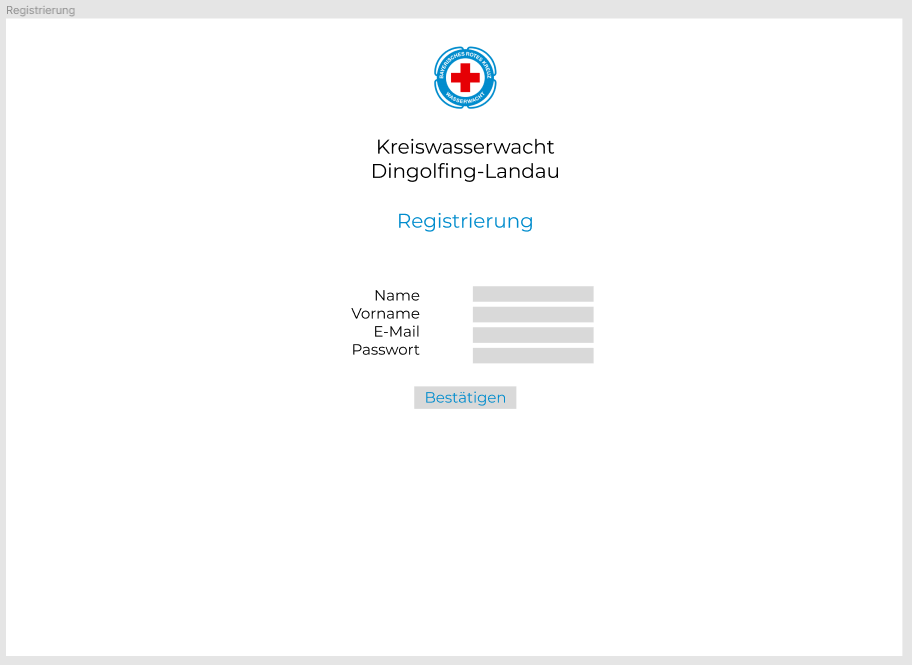
\includegraphics[width=\linewidth]{Anlagen/Figma/2-Registrierung.png}
    \caption{Registrierung}
  \end{subfigure}
  \begin{subfigure}[b]{0.4\linewidth}
    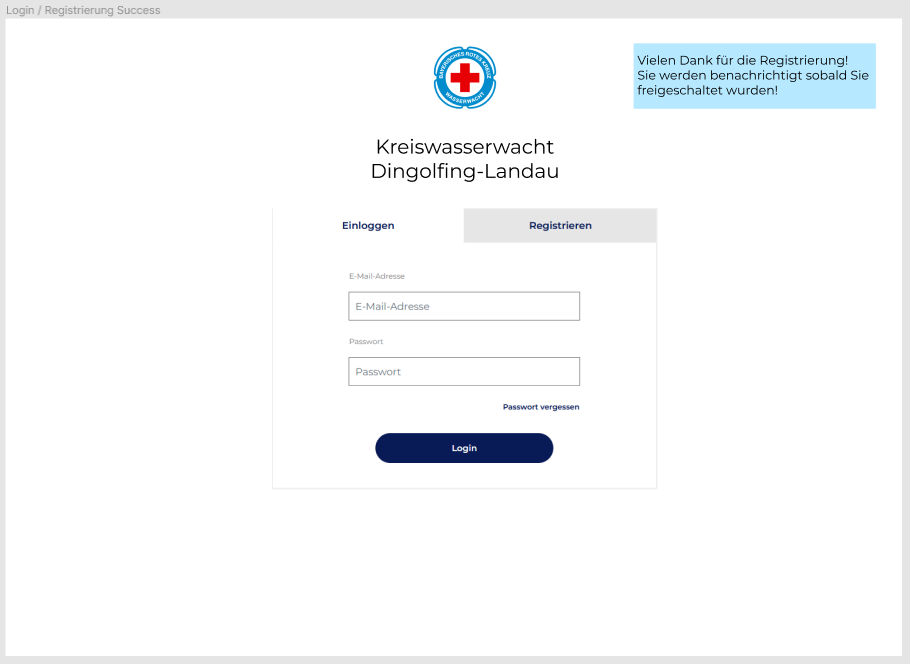
\includegraphics[width=\linewidth]{Anlagen/Figma/3-LoginSuccess.png}
    \caption{Benachrichtigung nach Registrierung}
  \end{subfigure}
  \caption{AnmeldeProzess}
  \label{fig:anmeldeprozess}
\end{figure}

%Nutzerübersicht
\subsubsection{Nutzerübersicht}
Admins sehen auf der Nutzerübersicht alle Benutzer und ob sie bereits freigeschaltet wurden. Über das jeweilige Profil können sie die Person über einen Button freischalten. Danach wird derjenige per Email benachrichtigt und erhält Zugang zum System. Außerdem soll für jedes Mitglied eine Statistik erhoben werden, wie viele Stunden im Dienst verbracht wurden. Dies wurde als Anforderung mit aufgenommen, wurde jedoch im Mock nicht mehr eingearbeitet sondern direkt in die tatsächliche Anwendung eingebaut.

\begin{figure}[H]
  \centering
  \begin{subfigure}[b]{0.4\linewidth}
    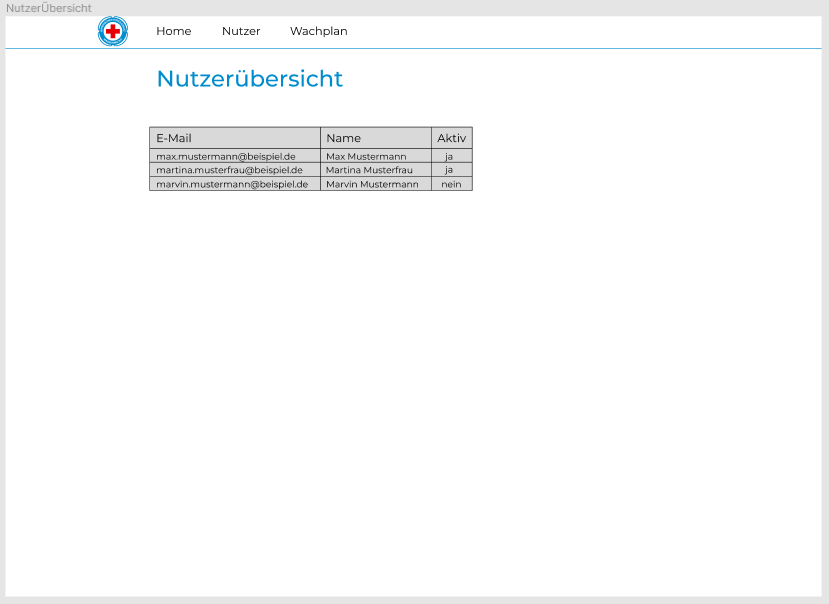
\includegraphics[width=\linewidth]{Anlagen/Figma/6-Nutzeruebersicht.png}
    \caption{Nutzerübersicht}
  \end{subfigure}
  \begin{subfigure}[b]{0.4\linewidth}
    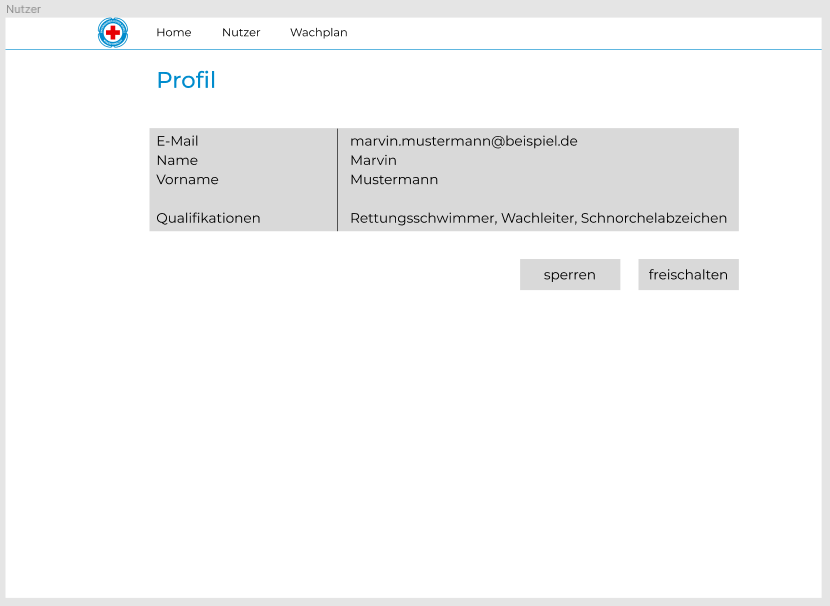
\includegraphics[width=\linewidth]{Anlagen/Figma/7-ProfilAdminSicht.png}
    \caption{Profil Admin Ansicht}
  \end{subfigure}
  \caption{Freischaltungs-Prozess}
  \label{fig:freischaltprozess}
\end{figure}

%Wachplan
\subsubsection{Wachplanung}
Bei der Wachplanung wurde angefordert, dass Wachtermine einzeln für ein bestimmtes Datum und Uhrzeit angelegt werden können. Außerdem soll es möglich sein gleich eine Reihe an Terminen anzulegen. Dazu muss ein Start- und Enddatum angegeben werden, die Uhrzeit, sowie die Wochentage an denen ein Termin eingestellt werden soll. \\
Als Übersicht für die bisherigen Termine wird ein Kalender verwendet. Hier wurde überlegt, ob man die einzelnen Termine farbig codiert, wenn beispielsweise ein \glqq Rettungsschwimmer\grqq{} und \glqq Wachleiter\grqq{} noch nicht eingebucht sind. In weiteren Abstimmungsterminen hat man sich aber darauf geeinigt, die Termine rot einzufärben, wenn noch niemand eingebucht ist, und grün einzufärben wenn Nutzer eingebucht sind.

\begin{figure}[H]
  \centering
  \begin{subfigure}[b]{0.7\linewidth}
    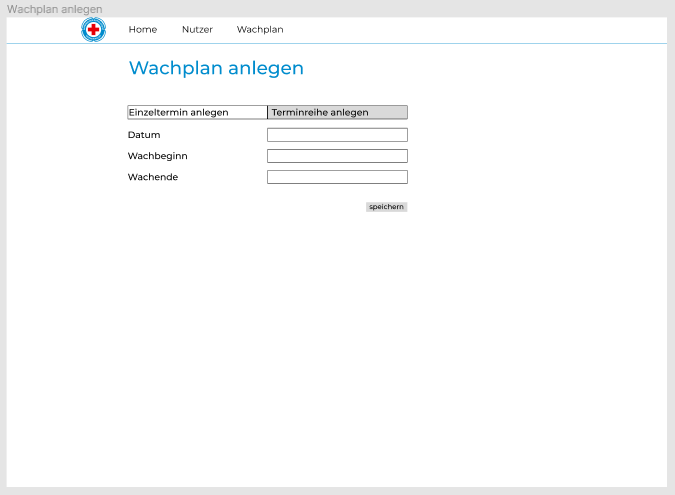
\includegraphics[width=\linewidth]{Anlagen/Figma/10-Wachplananlegen.png}
    \caption{Einzeltermin anlegen}
  \end{subfigure}
  \begin{subfigure}[b]{0.7\linewidth}
    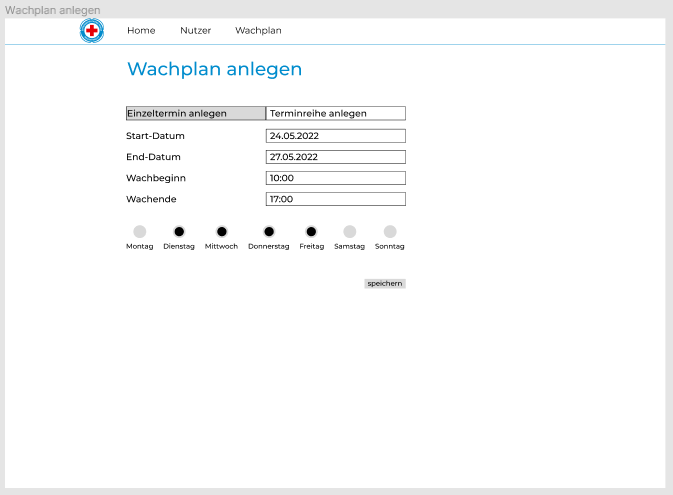
\includegraphics[width=\linewidth]{Anlagen/Figma/12-WachplanReiheAnlegenBef.png}
    \caption{Terminreihe anlegen}
  \end{subfigure}
  \begin{subfigure}[b]{0.7\linewidth}
    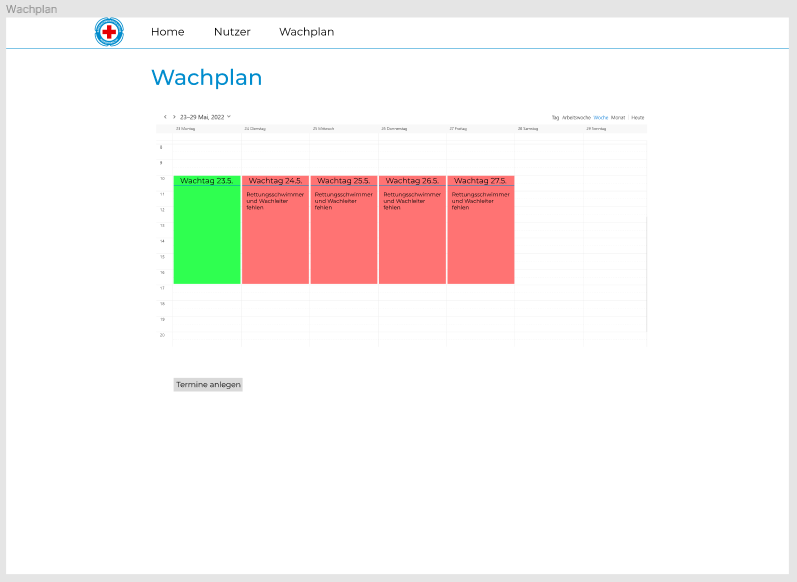
\includegraphics[width=\linewidth]{Anlagen/Figma/13-WachplanuebersichtAngelegt.png}
    \caption{Wachplan Übersicht}
  \end{subfigure}
  \caption{Wachplanung}
  \label{fig:wachplan}
\end{figure}

%Wachplandurchführung
\subsubsection{Wachplandurchführung}
Über einen Klick auf die Terminelemente im Wachplan kommt man auf die Durchführungsseite des jeweiligen Wachtages. Diese Seite wurde entsprechend der initialen Vorgabe $(siehe Anhang ~\ref{fig:initial})$ nachmodelliert. \\
Zunächst findet man oben auf der Seite das Tagesdatum, sowie die aktuelle Uhrzeit. Daneben findet man die Uhrzeit des Wachbeginns und Wachendes. \\
Rechts oben befindet sich die Ausgabe der aktuellen Wetterdaten, welche automatisch eingespielt werden sollen. Hierfür wurde nach einer passenden Wetter-Anwendung gesucht, welche eine API zur Abfrage der Daten bereitstellt. Darunter befindet sich ein Eingabefeld für die aktuelle Wassertemperatur. Diese wird von Wasserwachtmitgliedern gemessen und im System hinterlegt. \\ 
Nachfolgend befinden sich die Tabellen mit den Helfern für den Wachtag. Auf der linken Seite befindet sich die Tabelle mit den gebuchten Helfern. Ist ein Wachtag noch nicht gestartet, können sich Nutzer über ein darunter liegendes Eingabefeld einbuchen. Somit kann eine Planung der jeweiligen Wachtage stattfinden und man erhält einen Überblick, wie viele Personen planen vor Ort zu sein. Rechts daneben befindet sich die Tabelle der anwesenden Helfer. Sobald ein Wachtag gestartet wurde können sich die Nutzer über das selbe Eingabefeld einbuchen und ihren Wachbeginn dokumentieren. Hier wurde in weiteren Besprechungen noch angefordert, dass es möglich sein soll Nutzer aus einer Auswahlliste auszuwählen und einzubuchen und zusätzlich auch über ein Freitextfeld einzugeben. Die Möglichkeit Nutzer über einen Freitext hinzufügen zu können wird benötigt, da auch Helfer am Dienst teilnehmen können, die nicht im System als Nutzer registriert sind. \\
Über den Button unterhalb kann eine An- und Abmeldung in der ILS dokumentiert werden. Daneben befindet sich der Button zum starten und beenden eines Wachtages.\\
Darunter befindet sich ein größeres Texteingabefeld, wodurch Geschehnisse während des Wachtages im Wachbuch festgehalten werden können.\\
Das Wachbuch enthält alle Ereignisse eines Wachtages. Ein Eintrag enthält immer einen Zeitstempel und den jeweiligen Nutzer der den Eintrag verfasst hat, bzw \glqq System\grqq{} wenn der Eintrag automatisch eingefügt wurde. Das Wachbuch dokumentiert somit Wachbeginn und Ende, Wachbeginn und Ende der jeweiligen Nutzer, die Wetterdaten, die Wassertemperatur, An- und Abmeldungen im ILS, sowie eigene Ereignisangaben der Nutzer.\\
Ein Feature welches im Mock noch nicht dargestellt wurde ist das Drucken eines Wachtages. Nach Beendigung eines Wachtages soll es möglich sein die gesammelten Daten als PDF herunterzuladen. Dafür wurde ein Dokument bereitgestellt, welches aktuell benutzt wird um den Wachtag zu protokollieren. Nach dieser Vorlage soll auch das PDF erstellt werden mit den Daten aus dem System.

\begin{figure}[H]
  \centering
  \begin{subfigure}[b]{0.7\linewidth}
    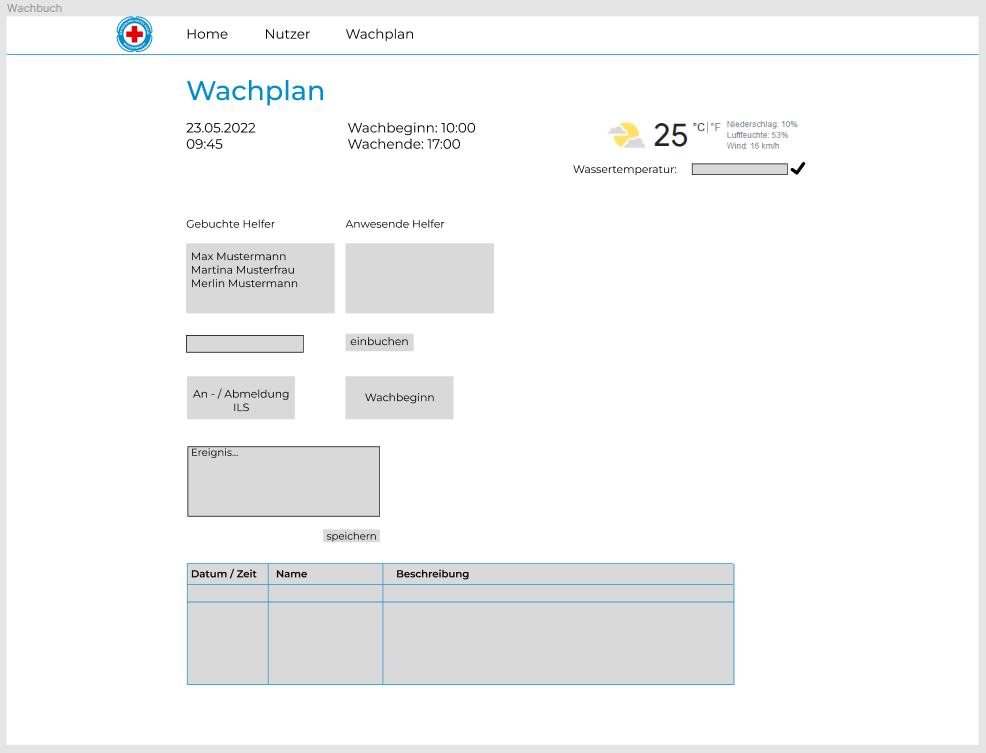
\includegraphics[width=\linewidth]{Anlagen/Figma/14-WachplanDurchfuehrung.png}
    \caption{Wachstart}
  \end{subfigure}
  \begin{subfigure}[b]{0.7\linewidth}
    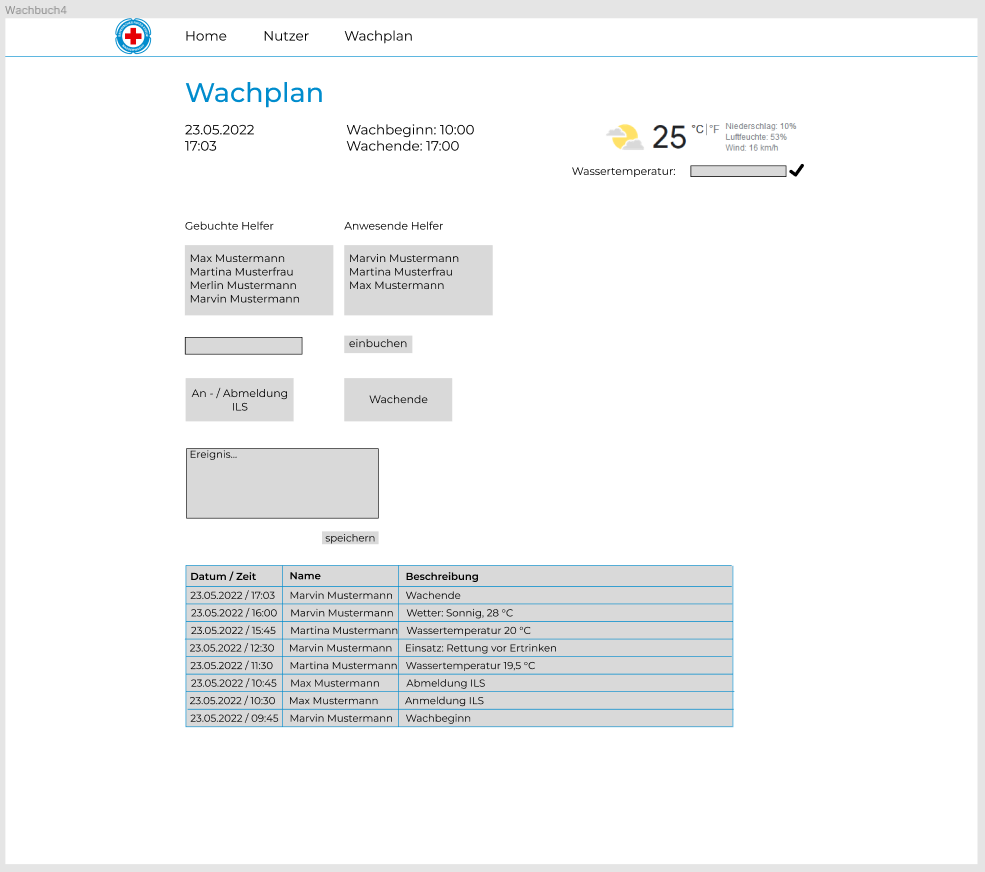
\includegraphics[width=\linewidth]{Anlagen/Figma/19-WachplanDurchfuehrung.png}
    \caption{Wachende}
  \end{subfigure}
  \caption{Wachbuch}
  \label{fig:wachbuch}
\end{figure}

%%%%%%%%%%%%%%%%%%%%%%%%%%%%%%%%%%%%
%
% Kapitel 4
%
%%%%%%%%%%%%%%%%%%%%%%%%%%%%%%%%%%%%
\renewcommand{\cleardoublepage}{}
\chapter{Technologien und Methoden}

\section{Auswahl geeigneter Technologien und Tools für die Webanwendung}
Bei der Auswahl der Technologien und Tools für die Entwicklung meiner Webanwendung habe ich mich bewusst für Tools entschieden, mit denen ich bereits praktische Erfahrung sammeln konnte. Während meines Entwicklungspraktikums an der Universität habe ich mit den gleichen Tools gearbeitet, nämlich Java als Programmiersprache, das Spring-Framework für die Backend-Entwicklung, Thymeleaf für die serverseitige HTML-Vorlagenverarbeitung und Bootstrap für das Frontend-Design. Diese praktische Erfahrung ermöglichte mir einen reibungslosen Start in das Projekt, da ich bereits mit den Konzepten, Funktionalitäten und bewährten Methoden dieser Tools vertraut war. Durch die Verwendung von Java und den genannten Frameworks konnte ich eine solide und effiziente Entwicklungsumgebung schaffen, um die Anforderungen der Webanwendung erfolgreich umzusetzen.
Im Folgenden werden die angewandten Technologien näher beschrieben.

\section{Beschreibung der verwendeten Programmiersprachen, Frameworks und Datenbanken}

\subsection{Java}
Java ist eine vielseitige und populäre Programmiersprache, die von Anfängern bis hin zu Profis genutzt wird. Sie zeichnet sich durch Einfachheit und Flexibilität aus und ermöglicht die Entwicklung komplexer Anwendungen.
%einfachheit und flexibilität, anfänger bsi profis

In Webanwendungen bietet Java mehrere Vorteile. Dank der objektorientierten Natur von Java können Entwickler einen wiederverwendbaren Code erstellen, was die Entwicklung und Wartung von Webanwendungen erleichtert. Java-Anwendungen sind plattformunabhängig, da sie auf einer virtuellen Maschine (JVM) laufen, was die Kompatibilität mit verschiedenen Betriebssystemen gewährleistet (vgl. \cite{scalosoftjava}).
%wiederverwendbarer Code; Plattformunabhängig JVM

Zusätzlich profitieren Entwickler von der breiten Unterstützung, einer großen Entwicklergemeinschaft und einer reichhaltigen Auswahl an Ressourcen (vgl. \cite{scalosoftjava}). Dies trägt dazu bei, effiziente und erfolgreiche Webanwendungen zu erstellen, die den Anforderungen der modernen Online-Welt gerecht werden.
%Große Community

\subsection{Spring}

Spring ist ein Open-Source Java Framework und bildet die Grundlage für dieses Projekt. Das Spring Framework wurde entwickelt um die Erstellung von Anwendungen zu erleichtern. \\
Kernfunktionalität von Spring ist die Inversion of Control (IoC) und die Dependency Injection (DI), die es ermöglicht, Abhängigkeiten zwischen Objekten zu verwalten. Durch die IoC kann eine Komponente Abhängigkeiten zu anderen Objekten definieren, ohne selbst diese Objekte instanziieren zu müssen. Der IoC Container fügt diese Abhängigkeiten dem Objekt ein (DI) (vgl. \cite{springioc}). \\
Das Spring-Framework deckt verschiedene Bereiche ab, darunter Webentwicklung, Datenbankzugriff, Sicherheit, Messaging und mehr. Spring Boot, eine Erweiterung von Spring, vereinfacht die Erstellung von Stand-alone-Anwendungen und Mikroservices, indem es eine vorkonfigurierte Umgebung bereitstellt (vgl. \cite{springboot}). \\
Ein weiterer Vorteil von Spring ist die große Community die dahinter steht. Für die verschiedenen Spring-Tools werden zahlreiche Tutorials und Dokumentation bereitgestellt, die eine große Hilfe für den Einstieg darstellen. 

Insgesamt erleichtert das Spring-Framework die Entwicklung von Java-Anwendungen erheblich, indem es bewährte Designmuster, Best Practices und Abstraktionen zur Verfügung stellt. Es ermöglicht es Entwicklern, sich auf die eigentlichen Funktionalitäten ihrer Anwendungen zu konzentrieren und gleichzeitig eine flexible, skalierbare und wartbare Architektur aufzubauen.

\subsection{Thymeleaf}

Thymeleaf ist eine leistungsstarke serverseitige Template-Engine für die Erstellung von Webseiten in Java-basierten Webanwendungen. Sie ermöglicht die nahtlose Integration von dynamischen Inhalten in HTML-Dokumente und erleichtert die Entwicklung von ansprechenden und interaktiven Benutzeroberflächen.

Ein herausragendes Merkmal von Thymeleaf ist seine Fähigkeit, direkt in HTML-Dokumenten zu arbeiten, wodurch die Integration von Serverdaten nahtlos erfolgen kann. Durch die Verwendung von speziellen Attributen und Tags in HTML-Dateien können Entwickler serverseitige Daten in die Darstellung einbetten und komplexe UI-Elemente erstellen.

Thymeleaf unterstützt verschiedene Template-Layouts, Fragmente und Iterationen, die die Wiederverwendbarkeit von Code fördern. Dies ermöglicht eine effiziente Entwicklung von konsistenten und wartbaren Benutzeroberflächen (vgl. \cite{thymeleaf}).

Ein weiterer Vorteil von Thymeleaf ist seine Integration mit Spring. Es passt nahtlos in das Spring-Framework und ermöglicht die einfache Verbindung von Daten aus dem Backend mit den Frontend-Templates. Dies erleichtert die Entwicklung von dynamischen Webseiten, ohne die Trennung zwischen Backend und Frontend zu beeinträchtigen (vgl. \cite{thymeleafspring}). 

Insgesamt bietet Thymeleaf eine effektive Möglichkeit, serverseitige Daten in HTML-Dateien zu integrieren und interaktive Webseiten zu erstellen. Es ist besonders gut in Kombination mit dem Spring-Framework geeignet und trägt zur Entwicklung von modernen und funktionalen Webanwendungen bei.

\subsection{Bootstrap}

Bootstrap ist ein Open-Source-Framework für das Frontend-Webdesign und die Entwicklung von responsiven und benutzerfreundlichen Benutzeroberflächen. Es wurde von Twitter entwickelt und stellt eine Sammlung von vorgefertigten HTML-, CSS- und JavaScript-Komponenten zur Verfügung, die Entwicklern helfen, schnell ansprechende Webseiten zu erstellen (vgl. \cite{twitterbootstrap}).

Ein herausragendes Merkmal von Bootstrap ist seine Fähigkeit zur Erstellung responsiver Designs. Das bedeutet, dass Webseiten, die mit Bootstrap erstellt werden, sich automatisch an verschiedene Bildschirmgrößen und Geräte anpassen können, darunter Desktops, Tablets und Smartphones. Dies trägt zur Verbesserung der Benutzererfahrung auf verschiedenen Plattformen bei (vgl. \cite{spurlock2013bootstrap}, S. 7).

Bootstrap bietet eine breite Palette von wiederverwendbaren UI-Komponenten wie Navigationsleisten, Buttons, Formularen, Karten, Modals und vieles mehr. Diese Komponenten können einfach in Webseiten integriert werden, wodurch die Entwicklung beschleunigt und konsistente Designs gewährleistet werden.
Das Framework enthält auch ein flexibles Rastersystem, das es Entwicklern ermöglicht, das Layout einer Webseite in Spalten und Zeilen zu strukturieren. Dies erleichtert die Erstellung komplexer Layouts und die Ausrichtung von Inhalten (vgl. \cite{bootstrapgrid}).

Bootstrap bietet auch vorgefertigte CSS-Klassen und JavaScript-Funktionalitäten, um häufig verwendete Funktionen wie Animationen, Navigation und Modals zu implementieren (vgl. \cite{bootstrapjs}). Dies ermöglicht es Entwicklern, interaktive Elemente ohne umfangreichen individuellen Code hinzuzufügen.

Insgesamt erleichtert Bootstrap die Entwicklung moderner Webseiten erheblich, indem es Entwicklern ermöglicht, schnell hochwertige und responsiv gestaltete Benutzeroberflächen zu erstellen. Es ist besonders nützlich für Projekte, die ein ansprechendes Design und eine konsistente Benutzererfahrung erfordern.

\subsection{Postgres \& Spring Data JPA}
%TODO Quellen suchen %

In meiner Bachelorarbeit habe ich PostgreSQL als Datenbankmanagementsystem (DBMS) verwendet, um die Daten meiner Webanwendung effizient zu speichern. Die Entscheidung für PostgreSQL als DBMS basierte auf seinen bewährten Funktionen für Datenpersistenz und -verwaltung (vgl. \cite{postgres}), sowie auf seiner nahtlosen Integration mit dem verwendeten Spring Data JPA-Framework (vgl. \cite{springdatajpa}).

PostgreSQL bietet eine solide Grundlage für die Datenpersistenz. In meiner Anwendung habe ich Daten in Form von Entitäten gespeichert. Entitäten sind Java-Klassen, die mit der Datenbanktabelle übereinstimmen und von Spring Data JPA verwaltet werden. Die Interaktion mit der Datenbank erfolgt durch objektorientierte Operationen, die von Spring Data JPA bereitgestellt werden (vgl. \cite{springdatajpaentities}). Dies ermöglicht es, Datenbankabfragen und -manipulationen auf einer höheren Abstraktionsebene zu handhaben.

Obwohl PostgreSQL eine breite Palette von erweiterten Funktionen bietet, die von räumlichen Abfragen bis zur Unterstützung komplexer Datentypen reichen (vgl. \cite{postgres}), habe ich mich auf die grundlegenden Aspekte der Datenpersistenz beschränkt. Dazu gehörten die Erstellung von Datenbanktabellen basierend auf meinen Entitäten, die Definition von Primärschlüsseln und Fremdschlüsselbeziehungen für die Datenintegrität, sowie die Verwendung von Indizes zur Optimierung von Abfragen.

Insgesamt ermöglichte die Kombination von PostgreSQL und Spring Data JPA eine effiziente und zuverlässige Datenpersistenz in meiner Webanwendung. Die solide Leistung von PostgreSQL und die praktische Abstraktion von Spring Data JPA erleichterten die Entwicklung und Wartung meiner Anwendung erheblich.

\subsection{Wetter API}
Um für einen Wachtag die aktuellen Wetter Daten speichern zu können, wurde eine Wetter-API integriert.

Die Integration der Wetter-API erforderte die Auswahl einer geeigneten API und die Einbindung der API-Anfragen in den Entwicklungsprozess. In meiner Bachelorarbeit habe ich mich für die API von VisualCrossing entschieden (s.h. \cite{weatherapi}), da sie zuverlässige und detaillierte Wetterdaten bereitstellt, die speziell auf den Standort der Wasserwacht zugeschnitten sind. Ein weiterer Vorteil dieser API ist, dass sie pro Tag 1000 Abfragen kostenfrei erlaubt.

Die Wetter-API ermöglichte es meiner Webanwendung, aktuelle Wetterdaten wie Temperatur, Luftfeuchtigkeit, Windgeschwindigkeit abzurufen. Diese wurden dann in die Benutzeroberfläche meiner Anwendung integriert, um den Benutzern leicht verständliche Informationen zur Verfügung zu stellen. Zusätzlich werden diese Daten auch automatisch in das Wachbuch geschrieben. So kann man auch nach Ende eines Wachtages die genauen Wetterverhältnisse nachvollziehen.

\section{Agile Entwicklungsmethoden zur Umsetzung des Projekts}

Die agile Umsetzungsmethode bildete das Rückgrat der Entwicklung meiner Webanwendung für die lokale Wasserwacht. In Anbetracht der sich ständig ändernden Anforderungen und der Notwendigkeit, schnell auf Feedback zu reagieren, erwies sich die Agile Methodik als äußerst geeignet, um Flexibilität und Effizienz in den Entwicklungsprozess zu integrieren.

In meiner Bachelorarbeit habe ich eine agile Herangehensweise gewählt, um die Entwicklung meiner Webanwendung zu steuern. Während ich mich von den Kernprinzipien agiler Methoden inspirieren ließ, habe ich die traditionellen Sprints mit festgelegten Zeiträumen nicht strikt umgesetzt. Stattdessen habe ich mich für eine iterative Vorgehensweise entschieden, bei der ich in einer bestimmten Zeitspanne so weit wie möglich gearbeitet habe und dann die Ergebnisse vorgestellt und diskutiert habe. 

Die regelmäßige Abstimmung mit den Mitgliedern der Wasserwacht ermöglichte es schnell auf neue Anforderungen und Feedback zu reagieren. Gleichzeitig konnte ich dadurch den Fokus auf eine kontinuierliche Weiterentwicklung und Verbesserung der Anwendung legen.

%%%%%%%%%%%%%%%%%%%%%%%%%%%%%%%%%%%%
%
% Kapitel 5
%
%%%%%%%%%%%%%%%%%%%%%%%%%%%%%%%%%%%%

\renewcommand{\cleardoublepage}{}
\chapter{Konzeption und Umsetzung}

\section{Detaillierte Beschreibung der Konzeption der Webanwendung}

\subsection{Datenmodell}

Für die Webanwendung ist es erforderlich die benötigte Datenmenge in einer Datenbank zu persistieren. Die einzelnen Entitäten habe ich in einem UML-Diagramm aufgezeichnet, um die Abhängigkeiten zwischen ihnen besser zu veranschaulichen. Anhand diesem werde ich im Folgenden das zu Grunde liegende Datenmodell beschreiben.

\begin{figure}[H]
  \centering
  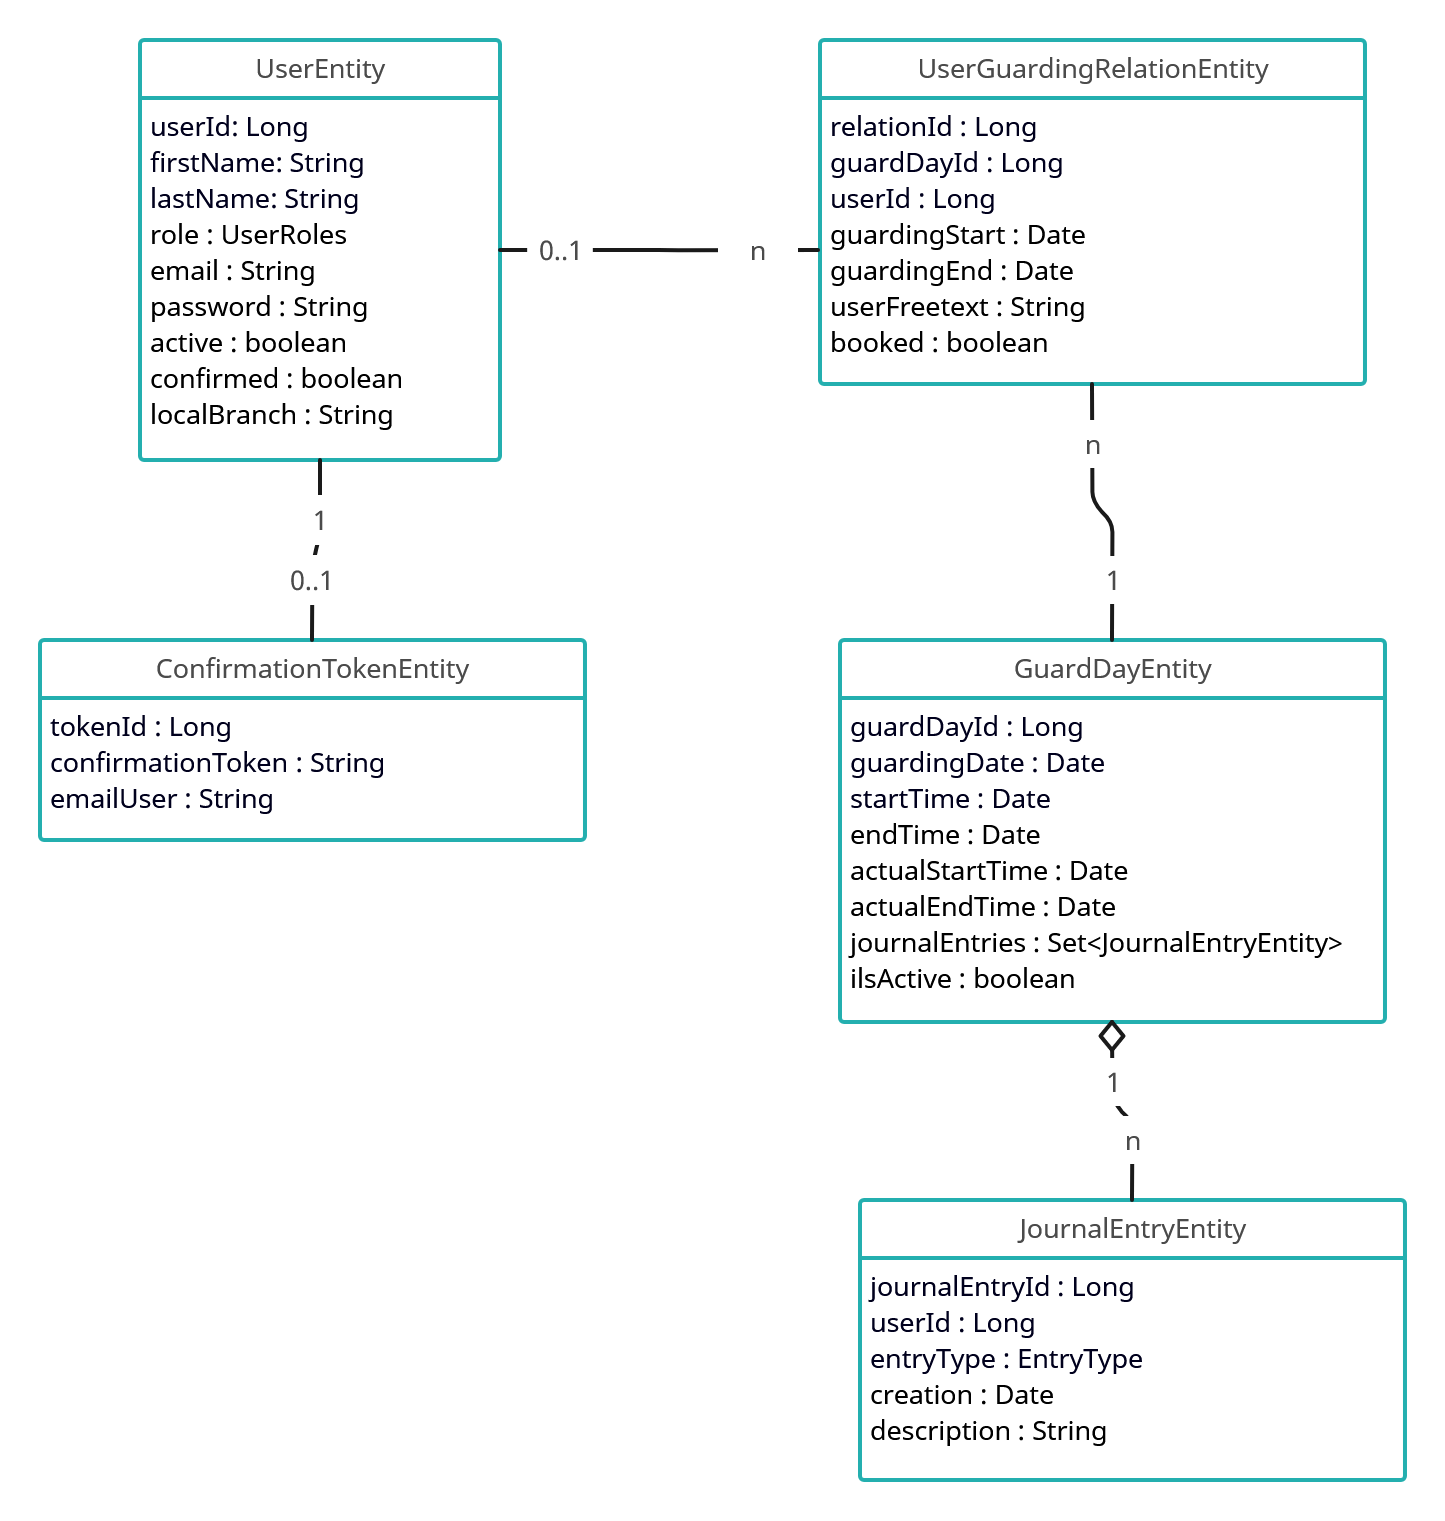
\includegraphics[width=0.6\linewidth]{Anlagen/umlDiagramm.png} 
  \caption{UML-Diagramm}
  \label{fig:anmeldeprozess}
\end{figure}

Zunächst kann festgestellt werden, dass jede Entität eine eindeutige Id besitzt. Diese dienen als Primärschlüssel der Entitäten, um eine eindeutige Identifikation zu ermöglichen.

\subsubsection{UserEntity}
Mit der \glqq UserEntity\grqq{} werden die Nutzerdaten repräsentiert. Zu Jedem Nutzer werden einige Kerndaten gespeichert, wie Vorname (\glqq firstName\grqq{}), Nachname (\glqq lastName\grqq{}), Email (\glqq email\grqq{}) und Passwort (\glqq password\grqq{}). Diese Daten dienen der Identifikation und Authentifizierung der Benutzer. \\
Die zugehörige Rolle eines Nutzers wird über das Attribut \glqq role\grqq{} repräsentiert. Dahinter steckt die Enumeration \glqq UserRoles\grqq{} mit den zugehörigen Werten \glqq ROLE\textunderscore USER\grqq{} und \glqq ROLE\textunderscore ADMIN\grqq{}. \glqq ROLE\textunderscore USER\grqq{} wird für einfache \glqq Mitglieder / Helfer\grqq{} verwendet, während \glqq ROLE\textunderscore ADMIN\grqq{} für \glqq Leitungskräfte / Admins\grqq{} verwendet wird. Mit der Rolle eines Benutzers werden Berechtigungen innerhalb der Anwendung gesteuert und Zugriffsschichten festgelegt. \\ 
Das Feld \glqq active\grqq{} spiegelt wieder, ob ein Anwender seine eigene Email-Adresse bei der Registierung bestätigt hat. Das Feld \glqq confirmed\grqq{} gibt wieder, ob der Nutzer durch einen Administrator freigeschaltet wurde. Wenn diese beiden Felder \glqq true\grqq{} sind, erhält der Nutzer Zugang zur Anwendung. Dadurch wird sichergestellt, dass keine unbefugten Personen Zugang zur Anwendung erhalten. \\
Über das Feld \glqq localBranch\grqq{} wird der jeweilige Ortsverband des Nutzers gespeichert.

\subsubsection{GuardDayEntity}
Über die \glqq GuardDayEntity\grqq{} werden die einzelnen Wachtage repräsentiert. Um einen Wachtag zu planen, braucht man ein Datum (\glqq guardingDate\grqq{}), einen geplanten Startzeitpunkt (\glqq startingTime\grqq{}) und einen geplanten Endzeitpunkt (\glqq endingTime\grqq{}). Wenn ein Wachtag dann tatsächlich gestartet wird, wird nochmal der genaue Startzeitpunkt gemessen und gespeichert (\glqq actualStartTime\grqq{}). Gleiches passiert auch beim Beenden mit dem Endzeitpunkt (\glqq actualEndTime\grqq{}). Über diese Zeitpunkte lässt sich auch der Status eines Wachtages bestimmen, also ob er noch in Planung ist, ob er gerade in der Durchführung ist, oder ob er bereits beendet wurde. \\ 
In \glqq journalEntries\grqq{} wird eine Liste der einzelnen Einträge im Wachbuch gespeichert. Dadurch sind die Einträge eindeutig einem Wachtag zugeordnet. Im Folgenden werden die \glqq JournalEntryEntities\grqq{}, die Bestandteile der \glqq journalEntries\grqq{} sind, genauer beschrieben. \\
Über das Feld \glqq ilsActive\grqq{} wird gespeichert ob gerade eine Verbindung zur integrierten Leitstelle vorhanden ist.  
 
 \subsubsection{JournalEntryEntity}
In der \glqq JournalEntryEntity\grqq{} werden die Einträge des Wachbuches festgehalten. Dazu wird einmal die \glqq userId\grqq{} gespeichert, die den Nutzer repräsentiert, der den Eintrag verfasst hat. Wird keine \glqq userId\grqq{} zu einem Eintrag gespeichert, kommt dieser Eintrag vom System selbst. Das passiert bei der automatischen Speicherung der Wetterdaten. \\
Jeder Eintrag hat einen \glqq EntryType\grqq{}, der angibt, um welche Art von Eintrag es sich handelt. Die verschiedenen Werte für \glqq EntryType\grqq{} sind in Tabelle \ref{tab:entrytype} aufgelistet. Dieser Typ erleichtert die Strukturierung und Kategorisierung der Einträge. Später werden bestimmte Kategorien gruppiert und im ausdruckbaren Wachbericht gesammelt dargestellt. \\
Außerdem werden pro Eintrag das Erstelldatum (\glqq creation\grqq{}) und der eigentliche Inhalt (\glqq description\grqq{}) gespeichert. So kann das Wachbuch chronologisch aufgebaut werden und ermöglicht es, die Ereignisse klar und detailliert zu dokumentieren.

\subsubsection{UserGuardingRelationEntity}
Damit sich Helfer bei einem Wachtag einbuchen können, ist es notwendig eine entsprechende Relation zwischen den beiden Entitäten herzustellen, die diesen Zustand speichern kann. Dazu wurde die \glqq UserGuardingRelationEntity\grqq{} modelliert. Sie enthält zunächst die \glqq userId\grqq{} des Nutzers und die \glqq guardDayId\grqq{} des jeweiligen Wachtages. Dadurch kann ein Nutzer eindeutig einem Wachtag zugeordnet werden. \\
Wenn sich ein Nutzer für einen Wachtag anmeldet, wird eine \glqq UserGuardingRelationEntity\grqq{} angelegt mit dem Attribut \glqq booked\grqq{}. Dies gibt an, dass sich ein Nutzer für diesen Wachtag einbucht und plant den Wachdienst an diesem Datum zu übernehmen. \\
Wenn ein Mitglied den Wachdienst antritt, wird eine neue Entität erstellt, um diesen Zustand zu dokumentieren. Diese Entität enthält das Attribut \glqq booked\grqq{}, das auf \glqq false\grqq{} gesetzt wird, um anzuzeigen, dass der Nutzer den Wachdienst angetreten hat. Ebenso werden der Wachbeginn (\glqq guardingStart\grqq{}) und das Wachende (\glqq guardingEnd\grqq{}) in dieser neuen Entität festgehalten. Dies ermöglicht die Unterscheidung zwischen den Nutzern, die sich für den Wachdienst eingebucht haben, und denjenigen, die tatsächlich anwesend sind. Die ursprüngliche \glqq UserGuardingRelationEntity\grqq{}, die die Einbuchung des Nutzers dokumentiert, bleibt dabei unverändert.\\
Da es auch vorkommen kann, dass Helfer die Wasserwacht unterstützen, die nicht im System hinterlegt sind, besteht die Möglichkeit diesen per Freitext zu erfassen (\glqq userFreetext\grqq{}). In diesem Fall bleibt das Attribut \glqq userId\grqq{} leer. 

\begin{table}[ht]
\centering
\caption{Enumerationswerte für \glqq EntryType\grqq{}}
\label{tab:entrytype}
\begin{tabular}{|c|c|}
\hline
Enumeration Wert & Bezeichnung \\
\hline
DEFAULT & Manuelle Meldung \\
WEATHER & Wetterbericht	 \\
WATER\_TEMP & Wassertemperatur \\
USER\_GUARD\_BEGIN & Wachanmeldung Nutzer\\
USER\_GUARD\_END & Wachabmeldung Nutzer\\
GUARD\_BEGIN & Wachbeginn\\
GUARD\_END & Wachende\\
ILS\_ACTIVE & Anmeldung ILS\\
ILS\_INACTIVE & Abmeldung ILS\\
\hline
\end{tabular}
\end{table}

\subsubsection{ConfirmationTokenEntity}
Die \glqq ConfirmationTokenEntity\grqq{} wird verwendet, um den Bestätigungsprozess für die Registrierung neuer Nutzer zu verwalten. Bei der Registrierung eines neuen Nutzers wird ein eindeutiger Bestätigungstoken (\glqq confirmationToken\grqq{}) generiert und dem Nutzer per E-Mail als Bestätigungslink zugesandt. Die verwendete Email wird dabei auch in der Entität gespeichert im Attribut \glqq emailUser\grqq{}. Der Bestätigungstoken dient dazu, die Echtheit der E-Mail-Adresse des Nutzers sicherzustellen und sicherzustellen, dass die Registrierung vom Inhaber der E-Mail-Adresse initiiert wurde.

Die \glqq ConfirmationTokenEntity\grqq{} spielt eine entscheidende Rolle bei der Sicherstellung der Authentizität der E-Mail-Adresse eines neuen Nutzers und gewährleistet somit die Integrität des Registrierungsprozesses.

%\subsection{Prozesse}

%\subsubsection{Registrierung}

%Der Bestätigungsprozess erfolgt wie folgt:

   % Ein neuer Nutzer registriert sich auf der Plattform und gibt seine E-Mail-Adresse an.

    %Die Anwendung generiert einen eindeutigen Bestätigungstoken und speichert diesen in der \glqq ConfirmationTokenEntity\grqq{} zusammen mit der E-Mail-Adresse des Nutzers.

    %Der generierte Bestätigungstoken wird in Form eines Bestätigungslinks an die angegebene E-Mail-Adresse des Nutzers gesendet.

    %Der Nutzer klickt auf den Bestätigungslink, der den Bestätigungstoken enthält.

    %Die Anwendung überprüft, ob der erhaltene Bestätigungstoken mit dem in der Datenbank gespeicherten Token übereinstimmt.

   % Wenn die Übereinstimmung erfolgreich ist, wird die E-Mail-Adresse des Nutzers bestätigt und er erhält Zugang zur Plattform.

%Parallel: 
%Email an Admins
%Admin logt sich ein 
%Nutzerübersicht
%Klick auf Profil von Nutzer
%freischalten


%\section{Architektur}

%\subsection{Spring Boot}

%Die Webanwendung basiert auf Spring Boot. Dies erm\"oglichte einen schnellen Start, da mit Spring Boot sehr schnell Stand-Alone Anwendungen bereit gestellt werden k\"onnen. 

%\subsection {Spring Security}


\section{Funktionalitäten und Features der Anwendung}

Im Folgenden werden die einzelnen Masken der fertigen Webanwendung präsentiert und erklärt.

\subsection{Spring Security}

Mithilfe von Spring Security kann festgelegt werden, welchen Nutzern welche Bereiche der Webanwendung zur Verf\"ugung stehen. Das ist notwendig um sicherzustellen, dass nur Leitungskr\"aften administrative Funktionalit\"aten angeboten werden. \\
Dazu muss eine \glqq Security Configuration\grqq{} angelegt werden, innerhalb der man den verschiedenen Rollen verschiedene Berechtigungen erteilen kann.
\begin{figure}[H]
  \centering
    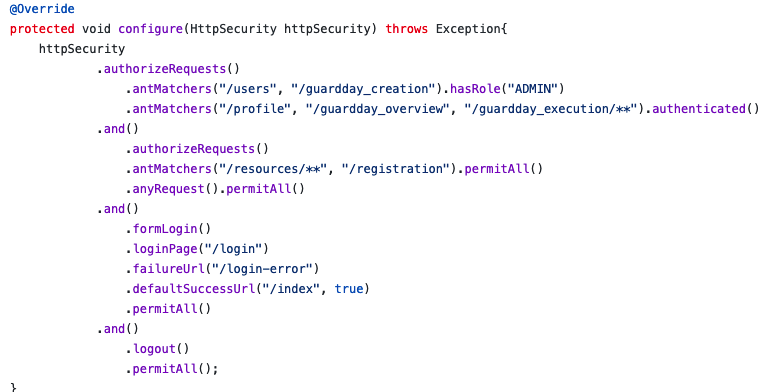
\includegraphics[width=0.7\linewidth]{Anlagen/Code/SecurityConfiguration.png}
    \caption{Auszug aus SecurityConfiguration.java}
  \label{fig:securityConfiguration}
\end{figure}

In diesem Fall wurde festgelegt, dass nur Admins auf die Bereiche \glqq Nutzer\"ubersicht\grqq{} und \glqq Wachtagerstellung\grqq{} zugreifen k\"onnen. Die Bereiche \glqq Profil\grqq{}, \glqq Wachtag\"ubersicht\grqq{} und \glqq Wachtagdurchf\"uhrung\grqq{} k\"onnen hingegen von jedem authentifizierten Anwender aufgerufen werden. \\
Weiterhin kann auf der Controller Ebene der Zugriff auf einzelne Request Mappings beschr\"ankt werden mit der Annotation \glqq PreAuthorize\grqq{}. 
\begin{figure}[H]
  \centering
    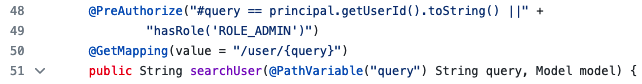
\includegraphics[width=0.7\linewidth]{Anlagen/Code/UserController.png}
    \caption{Auszug aus UserController.java}
  \label{fig:userController}
\end{figure}

Im Beispiel ~\ref{fig:userController} wird der Zugriff auf ein bestimmtes Profil nur gestattet, wenn der ausf\"uhrende Nutzer die Rolle Admin hat (\glqq hasRole('ROLE\_ADMIN')\grqq{}), oder der Anwender sein eigenes Profil sehen m\"ochte (\glqq query == principal.getUserId().toString()\grqq{}). \"Uber Principal kann auf den gerade authentifizierte Nutzer zugegriffen werden.

\subsection{Anmelde- / Registrierungsprozess}

Wenn man die Webanwendung das erste mal aufruft wird man auf die Login Seite geleitet. Besitzen die Helfer noch kein Konto, können sie sich über \glqq Registrieren\grqq{} einen neuen Account erstellen. Dazu geben sie ihre Email an, legen ein Passwort fest und erfassen die Daten zur Person. Durch Klick auf \glqq Registrieren\grqq{} wird ein neuer User angelegt und in der Datenbank gespeichert. In diesem Zustand kann der Nutzer die Website allerdings noch nicht betreten. \\
Im Hintergrund wird ein Bestätigungstoken generiert, der dem Anwender in Form eines Bestätigungslinks an die angegebene Email-Adresse versendet wird. Wenn man den Link aufruft, wird von der Anwendung überprüft, ob der erhaltene Bestätigungstoken mit dem in der Datenbank gespeicherten Token übereinstimmt. Wenn die Übereinstimmung erfolgreich ist, wird die Email-Adresse des Nutzers bestätigt. Somit wird sichergestellt, dass die Email-Adresse korrekt ist. \\
Parallel dazu wird an die hinterlegte Email-Adresse der Administratoren eine Email geschickt, um sie über eine neue Registrierung zu informieren. Sie müssen sich daraufhin im System anmelden und den Nutzer freischalten (siehe \ref{fig:anwendung-nutzerubersicht-admin}).

\begin{figure}[H]
  \centering
  \begin{subfigure}[b]{0.4\linewidth}
    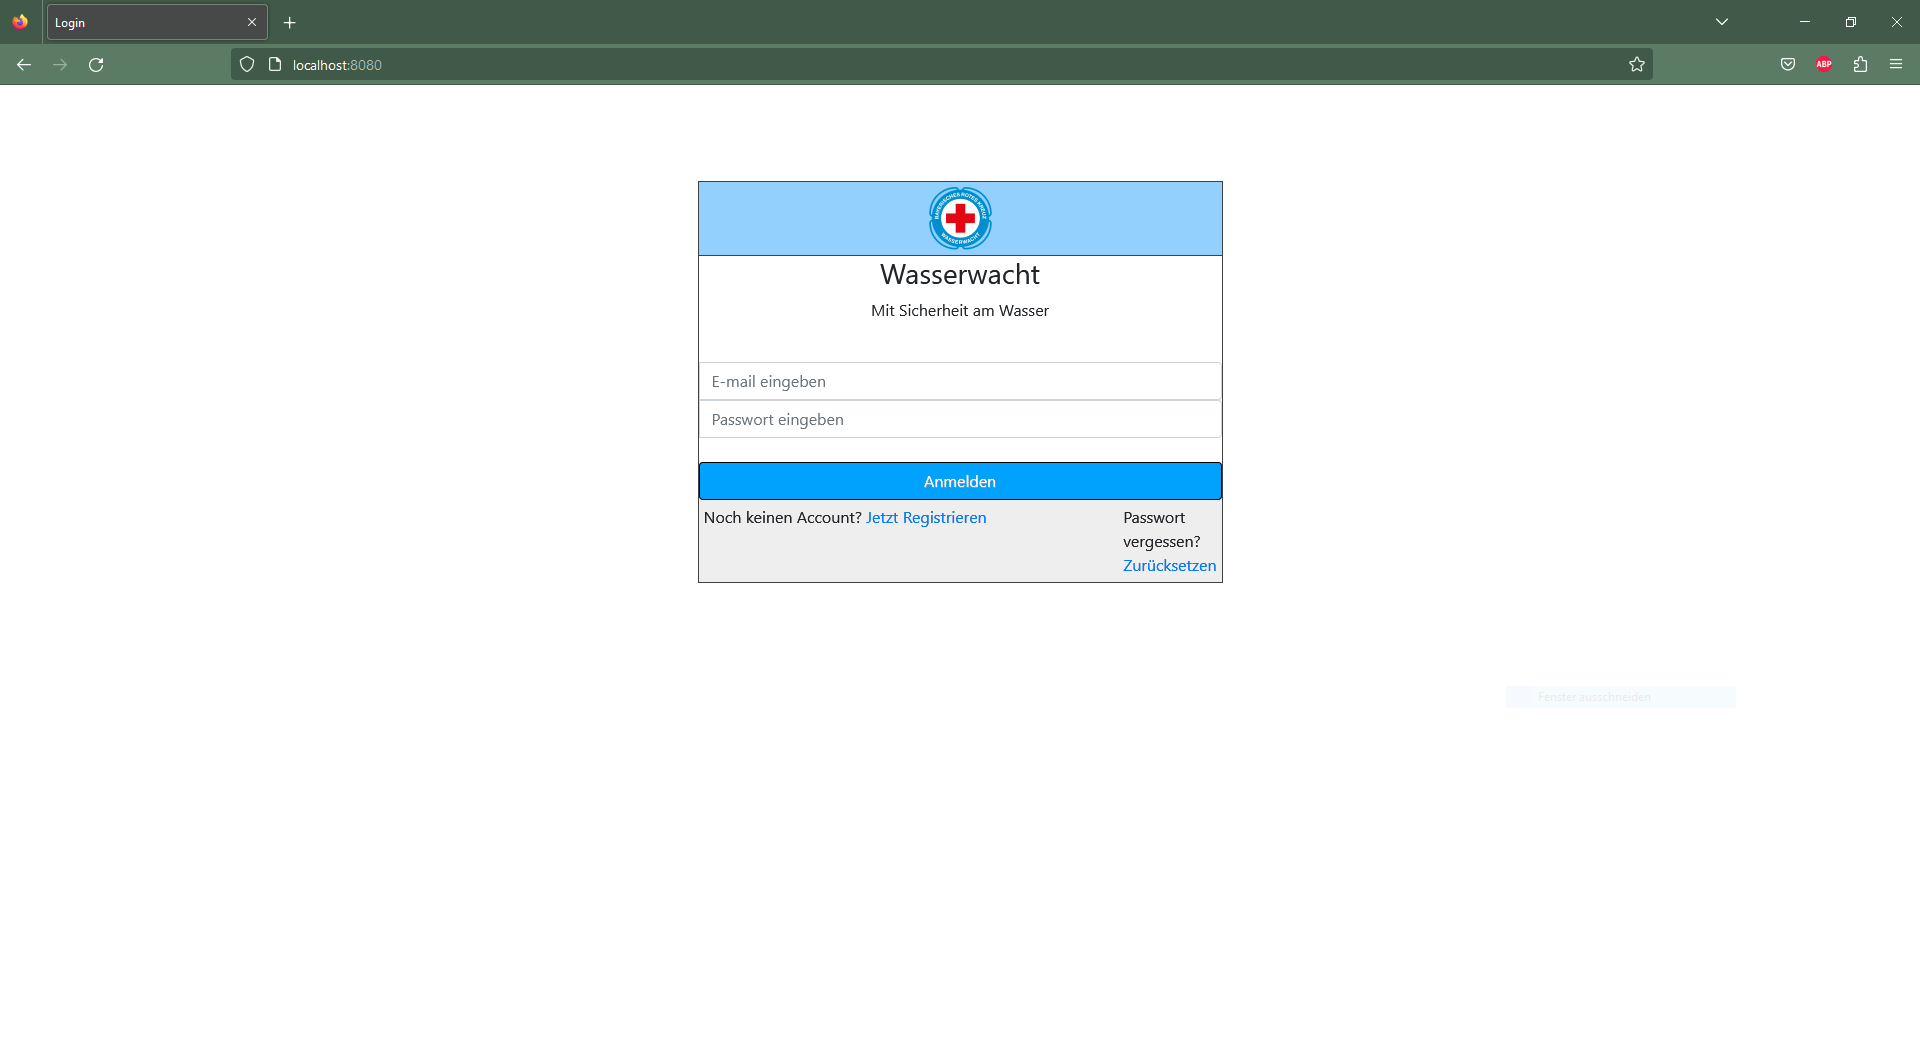
\includegraphics[width=\linewidth]{Anlagen/Anwendung/1Login.png}
    \caption{Login}
  \end{subfigure}
  \begin{subfigure}[b]{0.4\linewidth}
    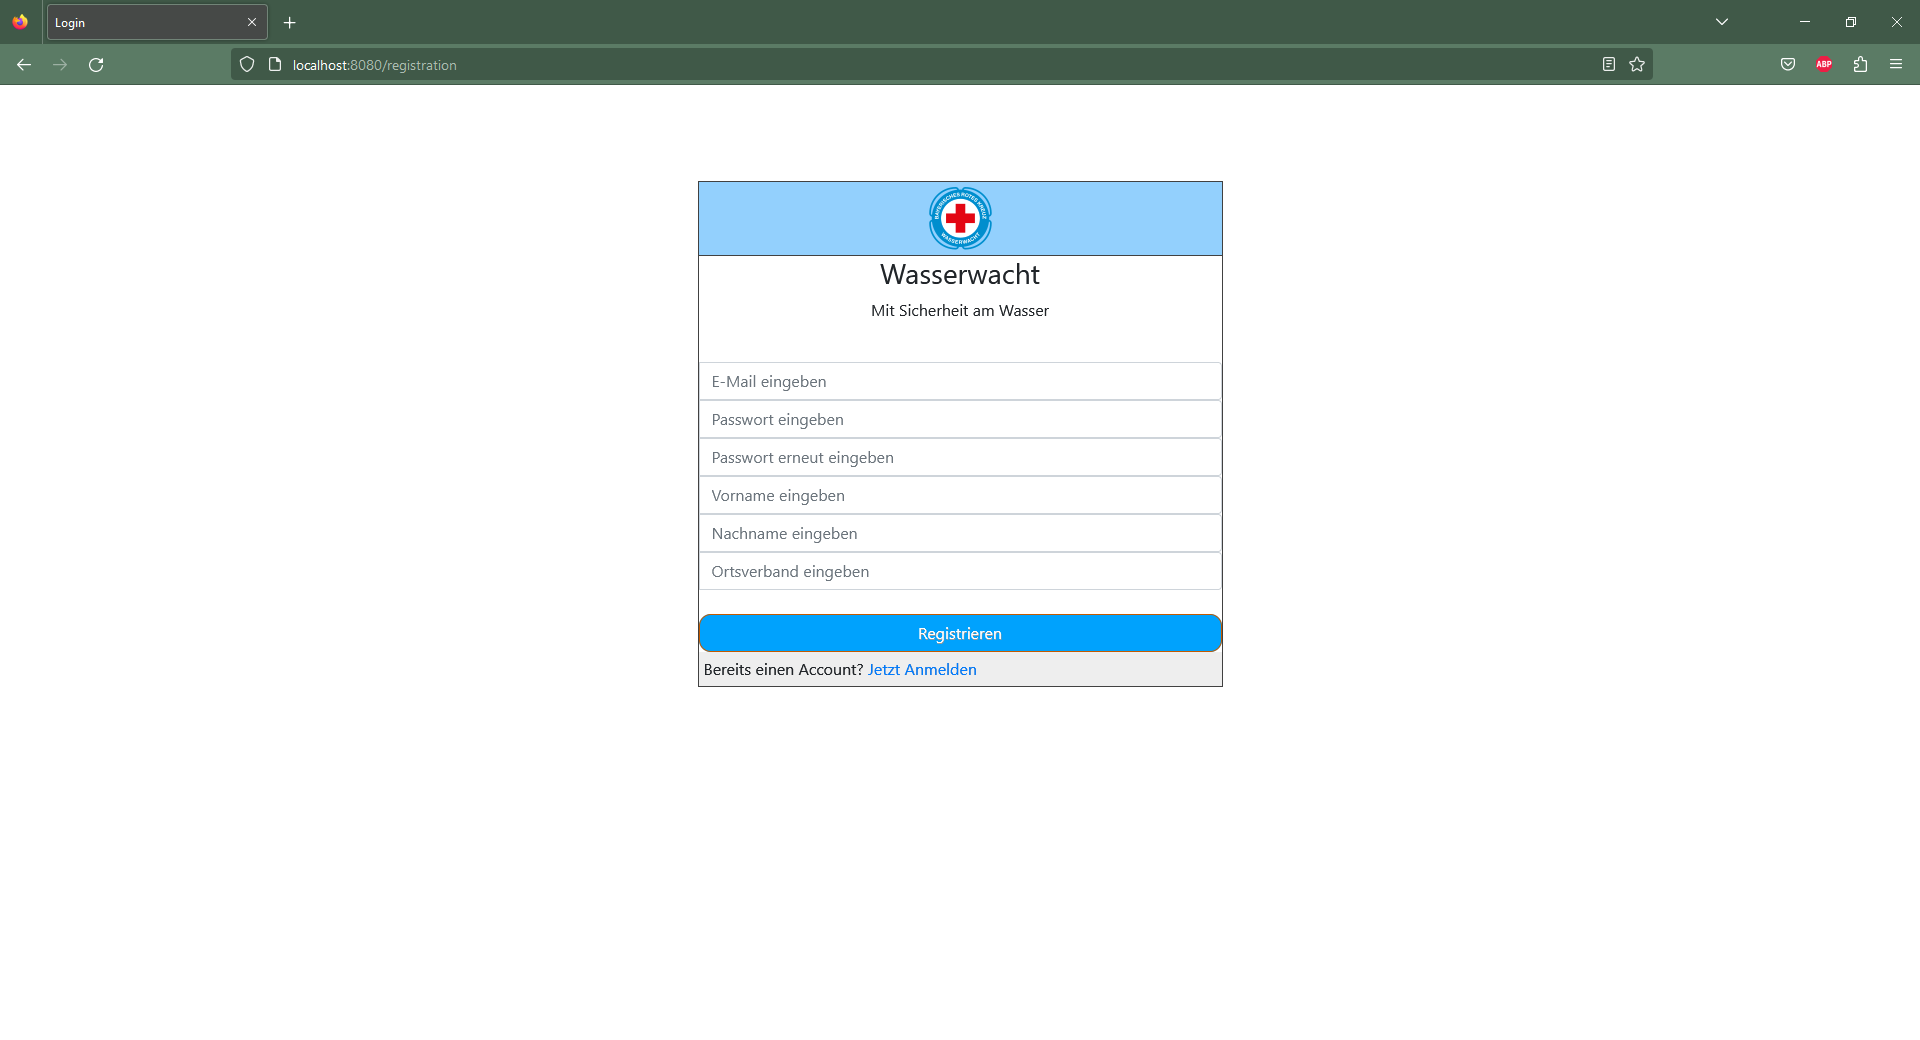
\includegraphics[width=\linewidth]{Anlagen/Anwendung/2Registrieren.png}
    \caption{Registrierung}
  \end{subfigure}
  \caption{AnmeldeProzess}
  \label{fig:anwendung-anmeldeprozess}
\end{figure}

\subsection{Navigationsleiste}

%F\"ur die Rollen \glqq User\grqq{} und \glqq Admin\grqq{} gibt es verschiedene Funktionalit\"aten innerhalb der Anwendung. Die Rollenverwaltung wurde mittels Spring Security umgesetzt. So kann sichergestellt werden, dass nur Leitungskr\"aften die administrativen Funktionalit\"aten zur Verf\"ugung stehen. Dies zeigt sich bereits in den unterschiedlichen Navigationsleisten, die je nach Rolle unterschiedliche verf\"ugbare Masken anzeigen. \\

Damit die Rollen \glqq User\grqq{} und \glqq Admin\grqq{} auch nur die Funktionalit\"aten angeboten kriegen, die sie verwenden d\"urfen, wurde die Navigationsleiste rollenspezifisch gestaltet (siehe \ref{fig:anwendungNavbars}). Normale Mitglieder haben \"uber die Navigationsleiste nur Zugang zu ihrem eigenen Profil und zur Wachtags\"ubersicht, w\"ahrend Administratoren zus\"atzlich noch Zugang zur Nutzer\"ubersicht und zur Wachtagserstellung haben.

\begin{figure}[H]
  \centering
  \begin{subfigure}[b]{0.5\linewidth}
    \fbox{
\includegraphics[width=\linewidth]{Anlagen/Anwendung/9NavbarUser.png}}
    \caption{Navigationsleiste - Nutzeransicht}
  \end{subfigure}
  \begin{subfigure}[b]{0.5\linewidth}
    \fbox{
\includegraphics[width=\linewidth]{Anlagen/Anwendung/9NavbarAdmin.png}}
    \caption{Navigationsleiste - Adminansicht}
  \end{subfigure}
  \caption{Navigationsleisten}
  \label{fig:anwendungNavbars}
\end{figure}

Dies konnte mit Hilfe von Thymeleaf's Integration von Spring Security umgesetzt werden. \"Uber das \glqq sec:authorize\grqq{} Attribut kann festgelegt werden, wann ein Element sichtbar ist. Im Beispiel ~\ref{fig:code-navbar} wird also der Men\"upunkt \glqq Profil\grqq{} nur den normalen Nutzern angezeigt, w\"ahrend den Admins eine Liste \glqq Nutzerverwaltung\grqq{} mit den Unterpunkten \glqq Profil\grqq{} und \glqq Nutzer\"ubersicht\grqq{} angezeigt wird.

\begin{figure}[H]
  \centering
    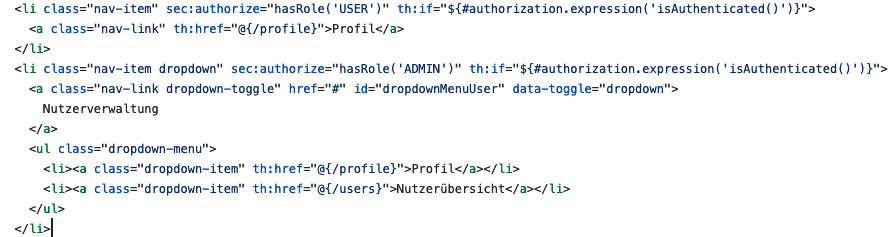
\includegraphics[width=0.7\linewidth]{Anlagen/Code/navbar.png}
    \caption{Auszug aus header.html}
  \label{fig:code-navbar}
\end{figure}

\subsection{Nutzerübersicht}

In der Anwendung haben Mitglieder die Möglichkeit ihre Profildaten einzusehen. Hier wird außerdem die Statistik ausgegeben, wie lange man schon im Wachdienst war. Die Statistik wird für jeden Nutzer berechnet, indem alle dem Nutzer zuordenbaren \glqq UserGuardingRelationEntities\grqq{} gelesen werden. Innerhalb einer Entit\"at kann dann mittels des Start- und Enddatums die jeweilige Dauer f\"ur den konkreten Wachtag berechnet werden.\\
Als Admin hat man zusätzlich eine Übersicht über alle registrierten Personen. Hier wird für jeden Nutzer die Statistik angegeben, die Rolle und ob der Nutzer schon aktiv ist. Wenn ein Nutzer noch nicht aktiviert wurde, kann ein Admin das Profil aufrufen und ihn über den Button \glqq Freischalten\grqq{} bestätigen. So wird sichergestellt, dass keine unbefugten Personen Zugang zum System erhalten.

\begin{figure}[H]
  \centering
  \begin{subfigure}[b]{0.5\linewidth}
    \fbox{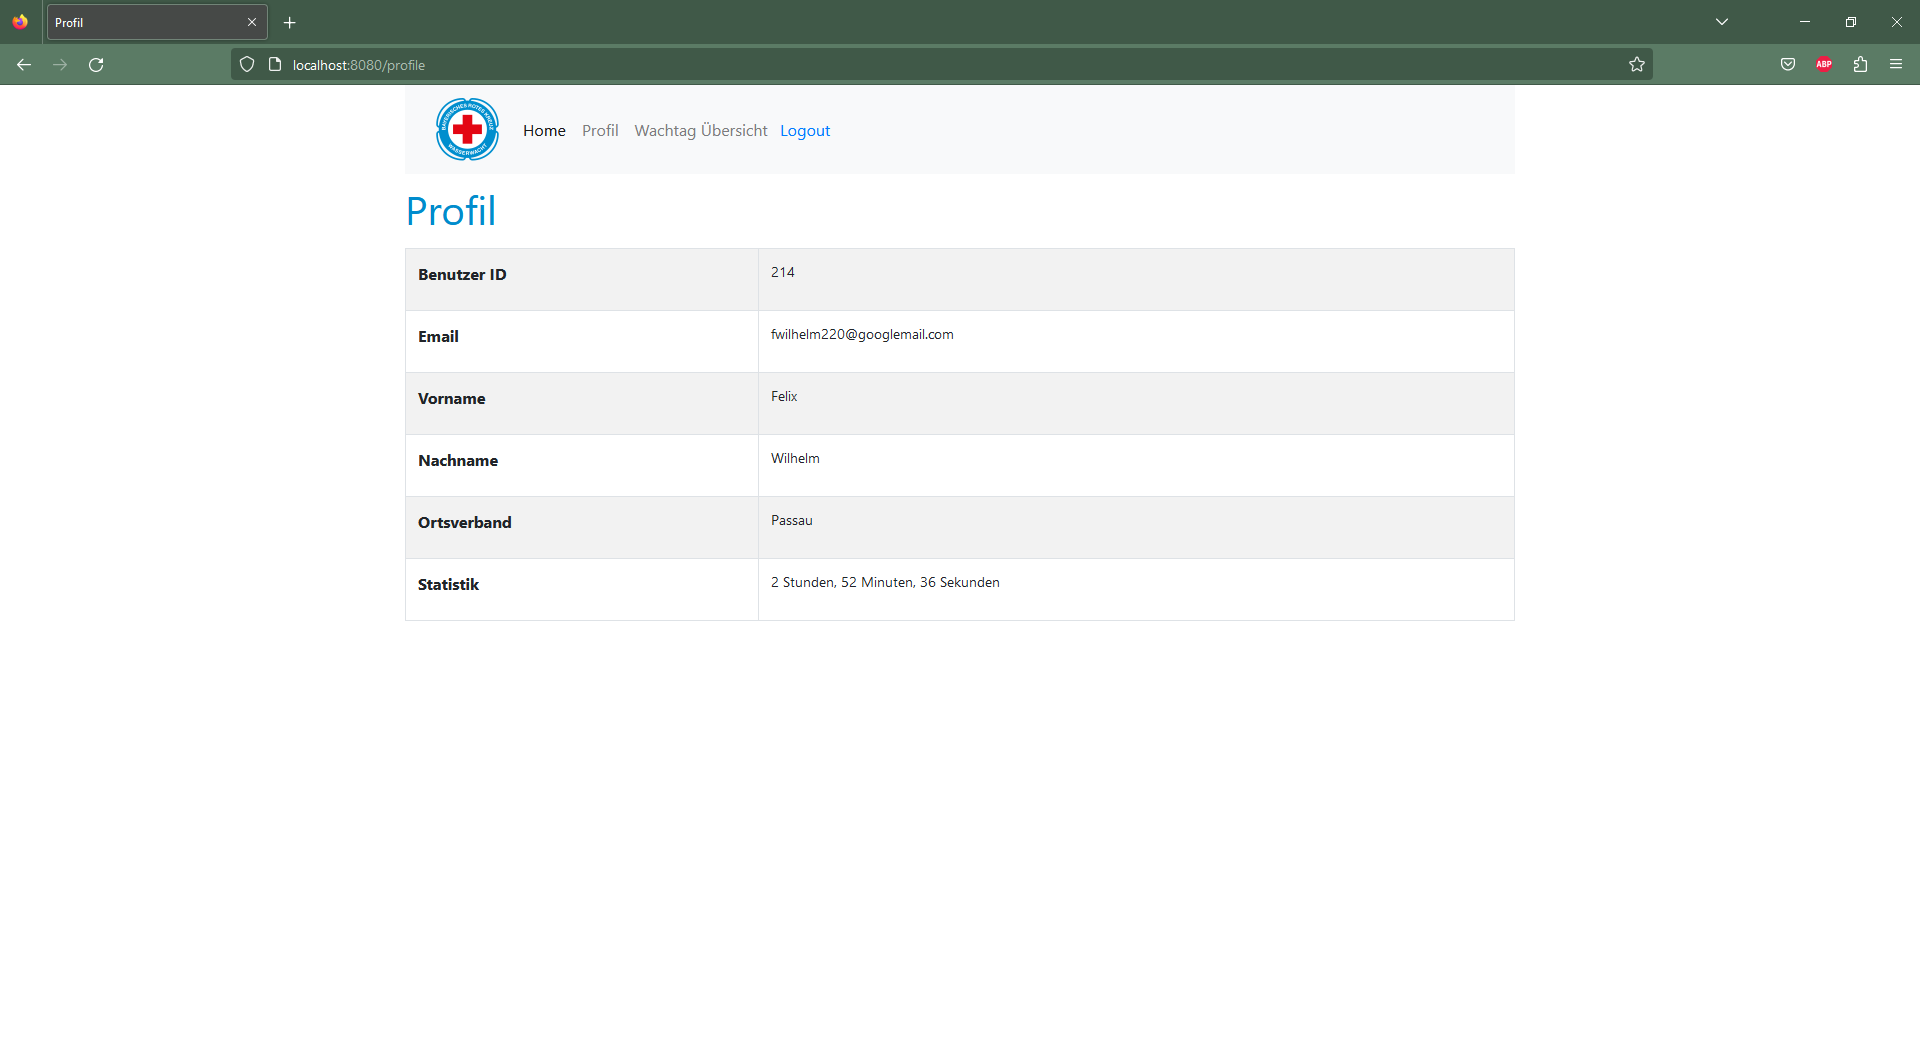
\includegraphics[width=\linewidth]{Anlagen/Anwendung/4ProfilNutzer.png}}
    \caption{Profil - Nutzeransicht}
  \end{subfigure}
  \begin{subfigure}[b]{0.5\linewidth}
    \fbox{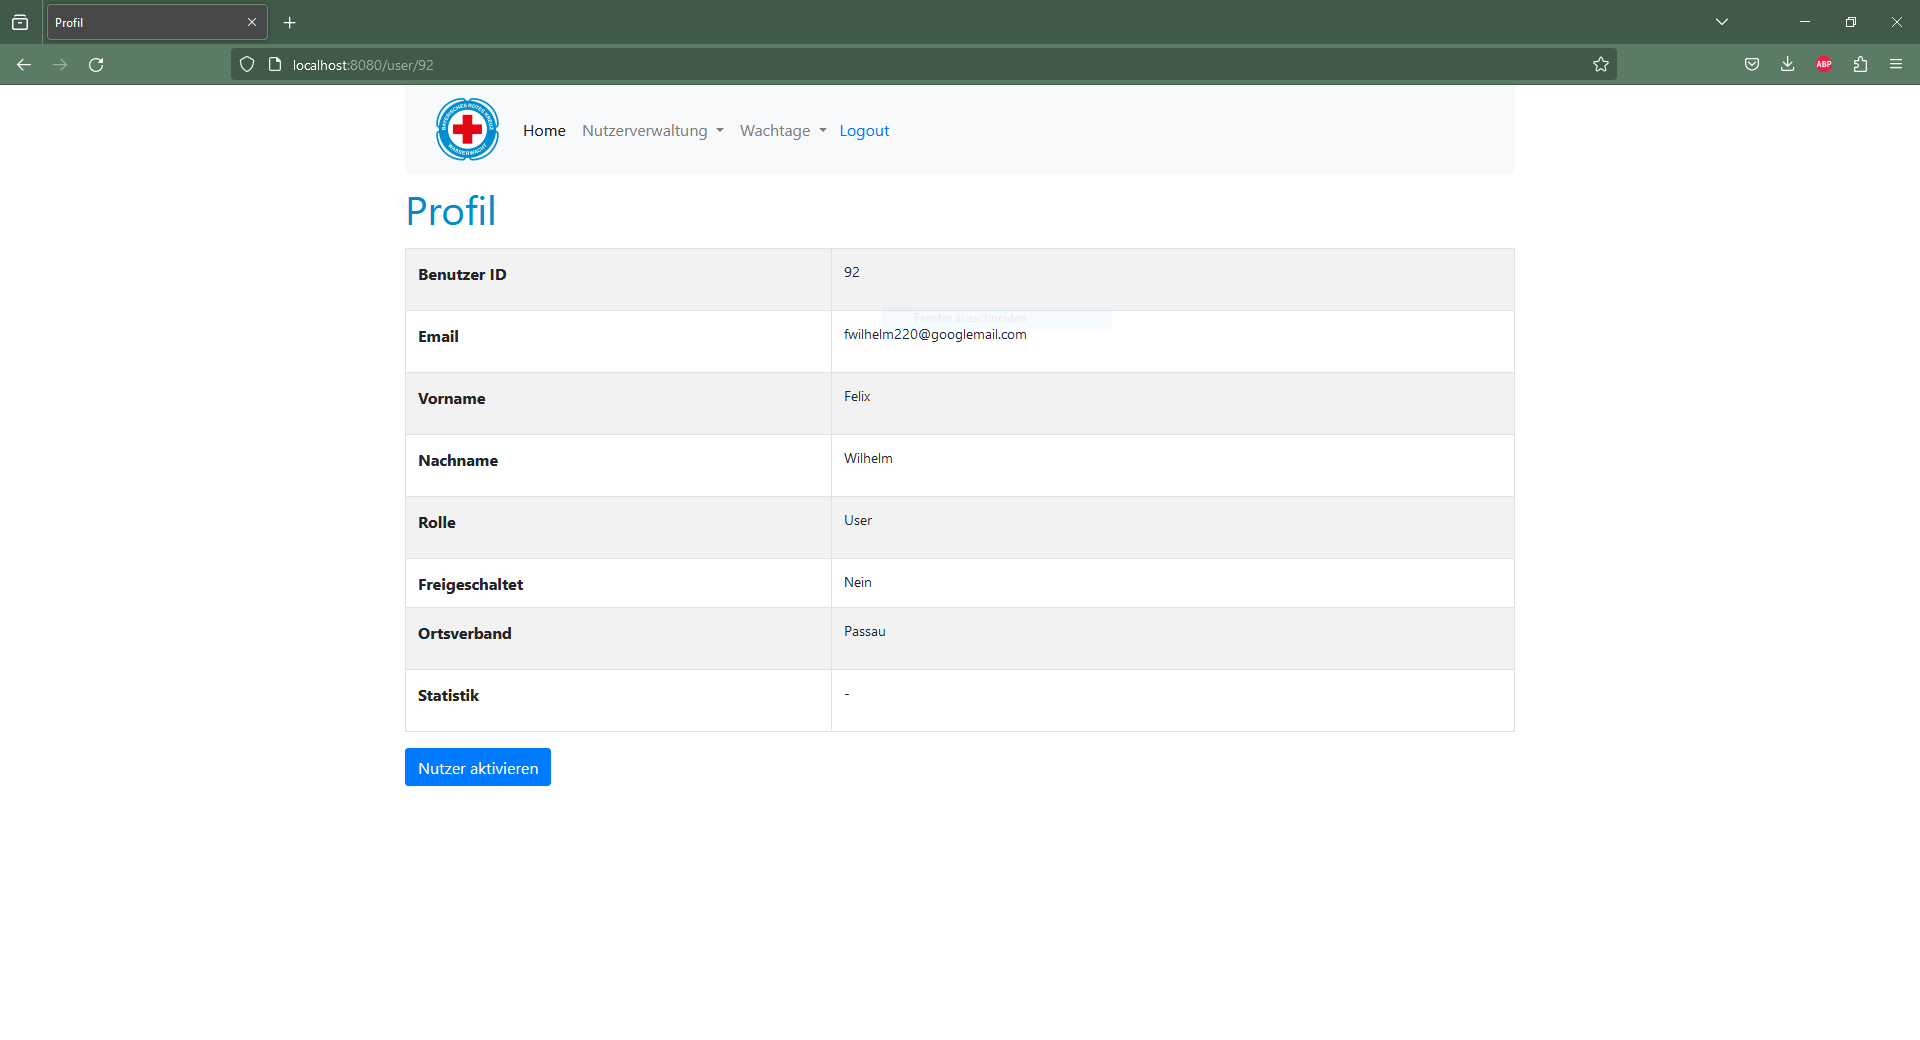
\includegraphics[width=\linewidth]{Anlagen/Anwendung/4ProfilAdmin.png}}
    \caption{Profil - Adminansicht}
    \label{fig:anwendung-nutzerubersicht-admin}
  \end{subfigure}
  \begin{subfigure}[b]{0.5\linewidth}
    \fbox{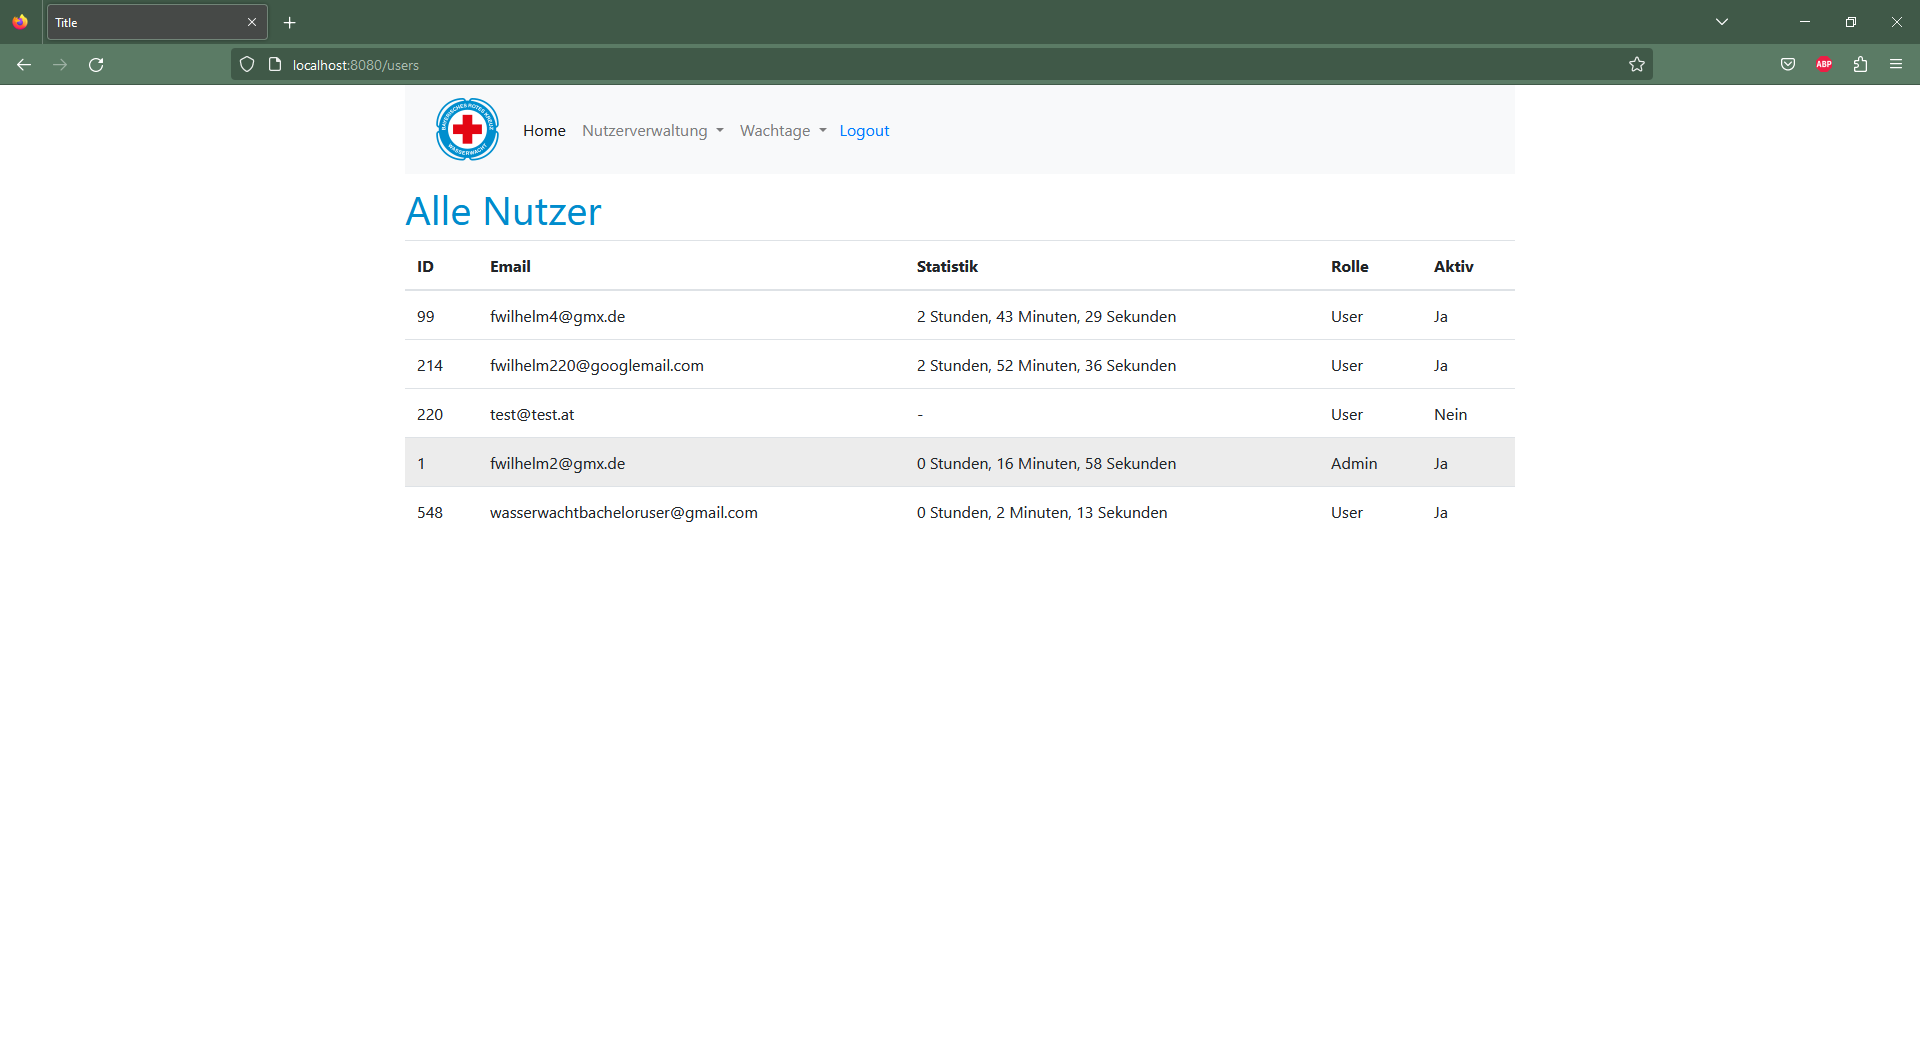
\includegraphics[width=\linewidth]{Anlagen/Anwendung/5Nutzerubersicht.png}}
    \caption{Nutzerübersicht}
  \end{subfigure}
  \caption{Nutzerübersicht}
  \label{fig:anwendung-nutzerubersicht}
\end{figure}

\subsection{Wachplanerstellung}

Bei der Wachplanerstellung gibt es zum Einen die M\"oglichkeit f\"ur einen einzelnen Termin einen Wachtag zu erstellen. Hier muss ein Datum, sowie Start- und Endzeitpunkt angegeben werden. Aus diesen Daten wird eine \glqq GuardDayEntity\grqq{} generiert und in der Datenbank gespeichert. 

\begin{figure}[H]
  \centering
    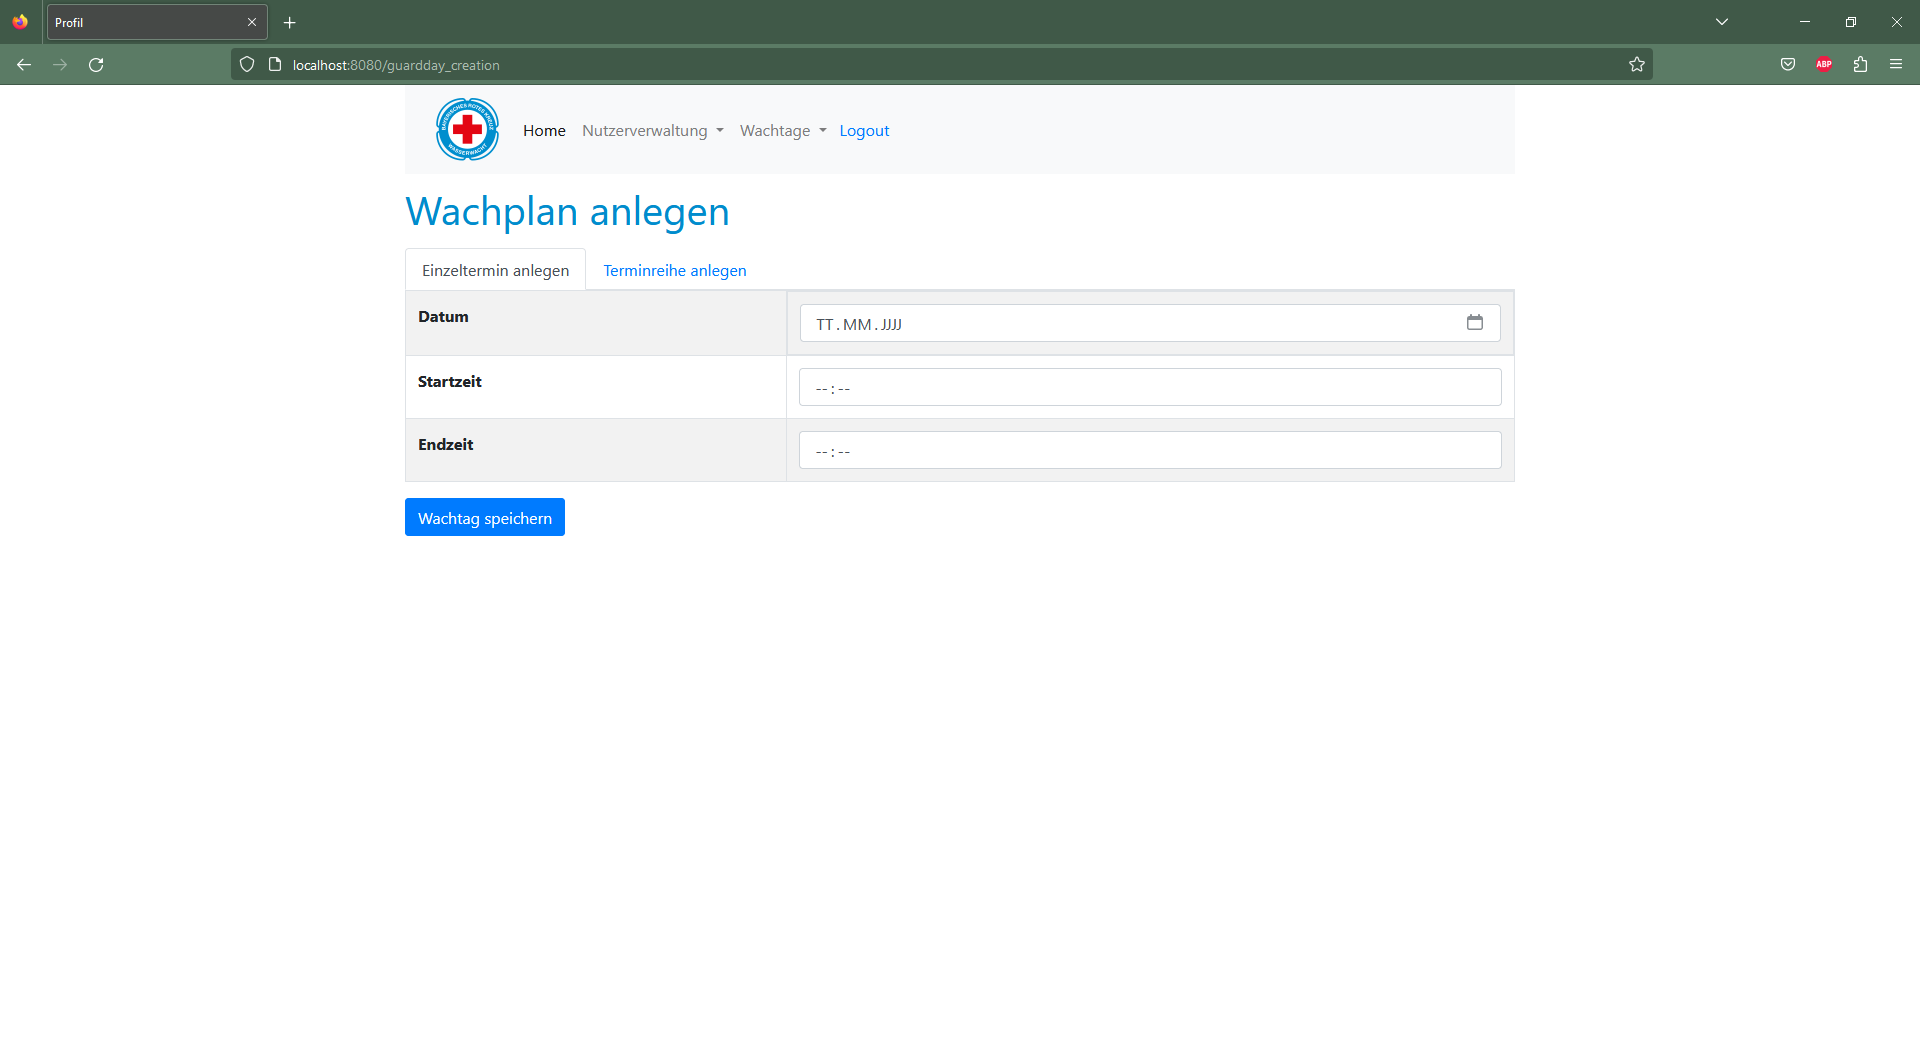
\includegraphics[width=0.7\linewidth]{Anlagen/Anwendung/6WachplananlegenSingle.png}
    \caption{Einzeltermin anlegen}
  \label{fig:anwendung-wachplanSingle}
\end{figure}

Es gibt au{\ss}erdem die M\"oglichkeit gleich eine Reihe an Wachtagen generieren zu lassen. Dazu muss ein Start- und Enddatum der Reihe angegeben werden, sowie wieder ein Start- und Endzeitpunkt. Zus\"atzlich m\"ussen die Tage ausgew\"ahlt werden, an denen ein Wachtag stattfinden soll. So wird f\"ur jeden ausgew\"ahlten Tag innerhalb diesen Zeitraums eine \glqq GuardDayEntity\grqq{} abgeleitet und abgespeichert.

\begin{figure}[H]
  \centering
    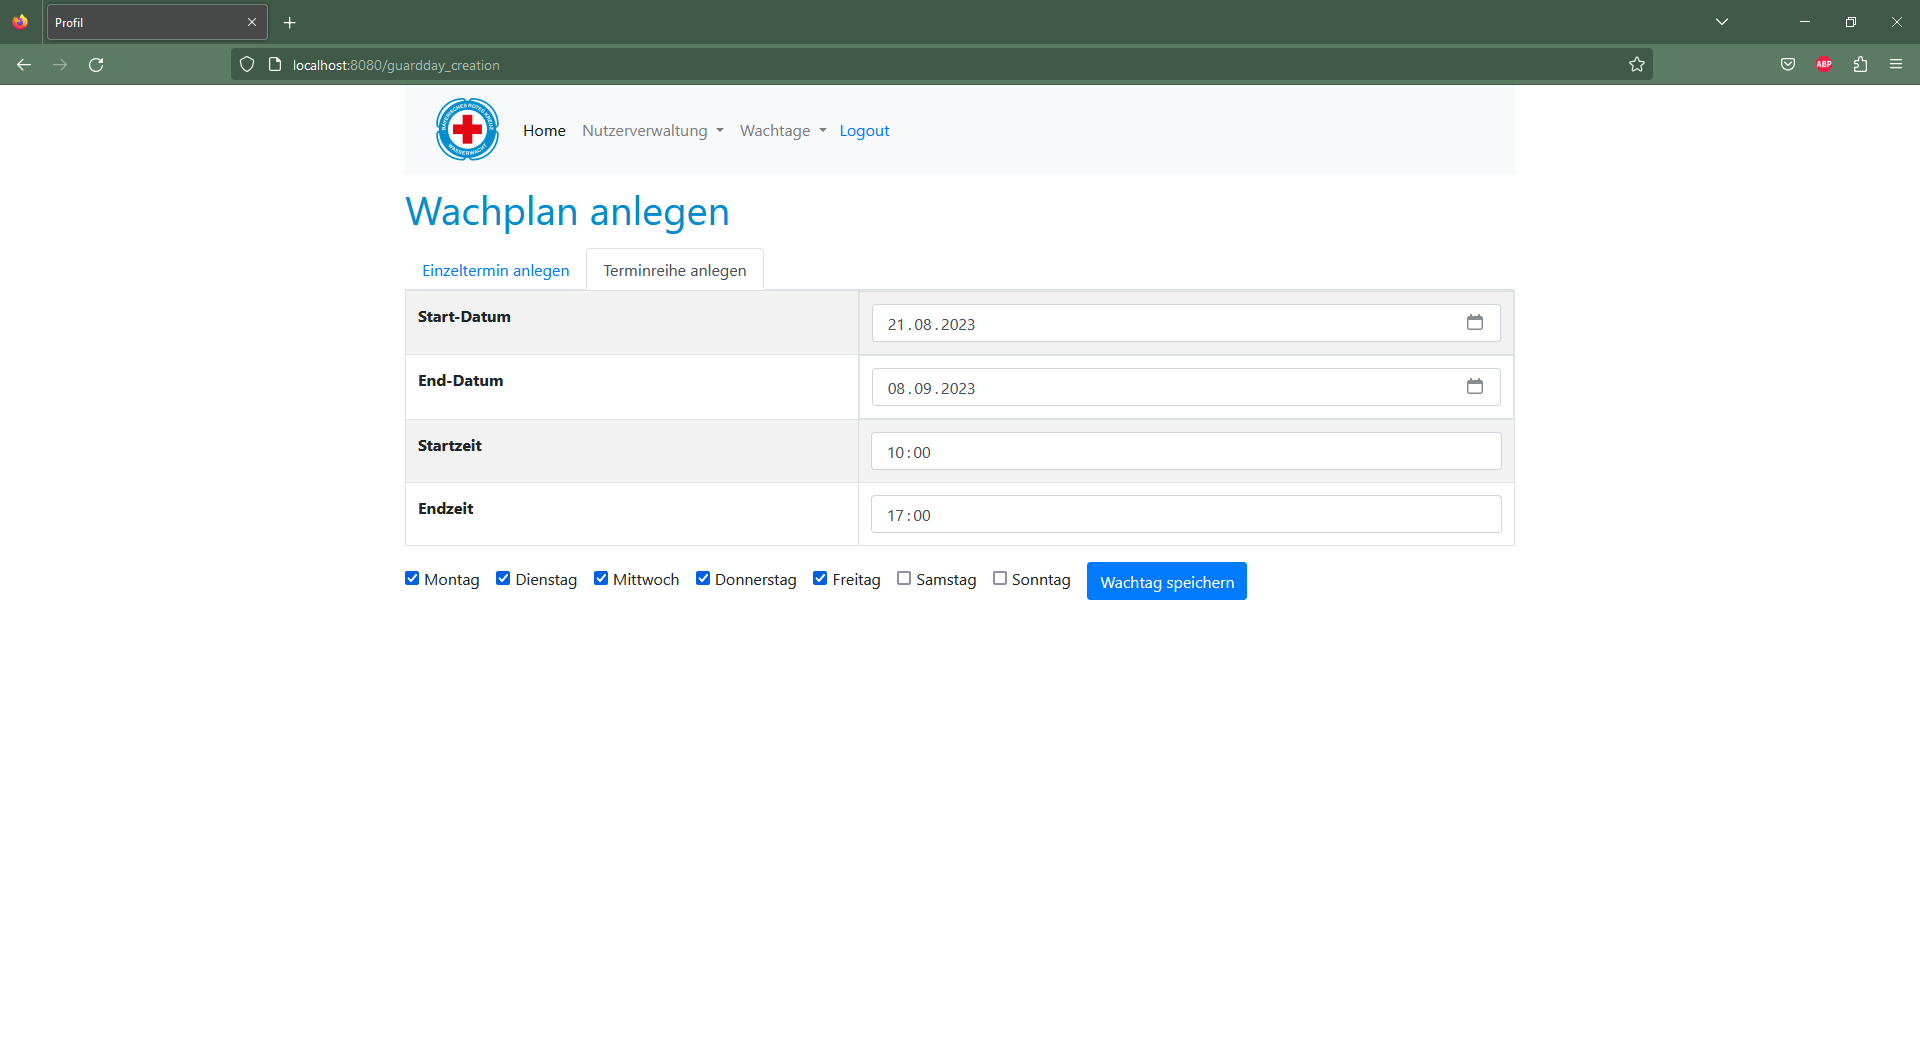
\includegraphics[width=0.7\linewidth]{Anlagen/Anwendung/6WachplananlegenMultipleBefullt.png}
    \caption{Terminreihe anlegen}
  \label{fig:anwendung-wachplanMultiple}
\end{figure}

\subsection{Wachplanübersicht}

Auf der Wachtag\"ubersicht $(siehe~\ref{fig:anwendung-wachubersicht})$ werden die verf\"ugbaren Wachtage in Kalenderform dargestellt. Diese werden an ihrem Datum in ihren Start und Endzeitpunkte dargestellt. Zus\"atzlich gibt es f\"ur jeden Tag eine farbige Codierung um \"uber den Zustand zu erfahren. Ist ein Wachtag rot hinterlegt, ist noch niemand f\"ur dieses Datum eingebucht. Ist ein Wachtag gr\"un hinterlegt, ist mindestens eine Person eingebucht. Wenn ein Wachtag abgeschlossen wurde, wird er grau hinterlegt. Dies erm\"oglicht es den Leitungskr\"aften auf einen Blick zu erkennen, bei welchen Wachtagen noch Personalmangel herrscht. \\
Um den Kalender darzustellen wurde das Open-Source Plugin \glqq jquery-calendar\grqq{} der Firma \glqq Arrobe\grqq{} verwendet. Dieser ließ sich sehr gut in die bestehende Anwendung integrieren und bietet die M\"oglichkeit, Termine farbig zu hinterlegen. Ein weiteres Feature dieses Kalenders ist das bestehende Responsive-Design. Der Kalender funktioniert auf einem Mobiltelefon ebenso gut wie auf einem Desktop-Computer. \\
\"Uber einen Klick auf ein Termin-Element gelangt man zur Seite des jeweiligen Wachtages.

\begin{figure}[H]
  \centering
    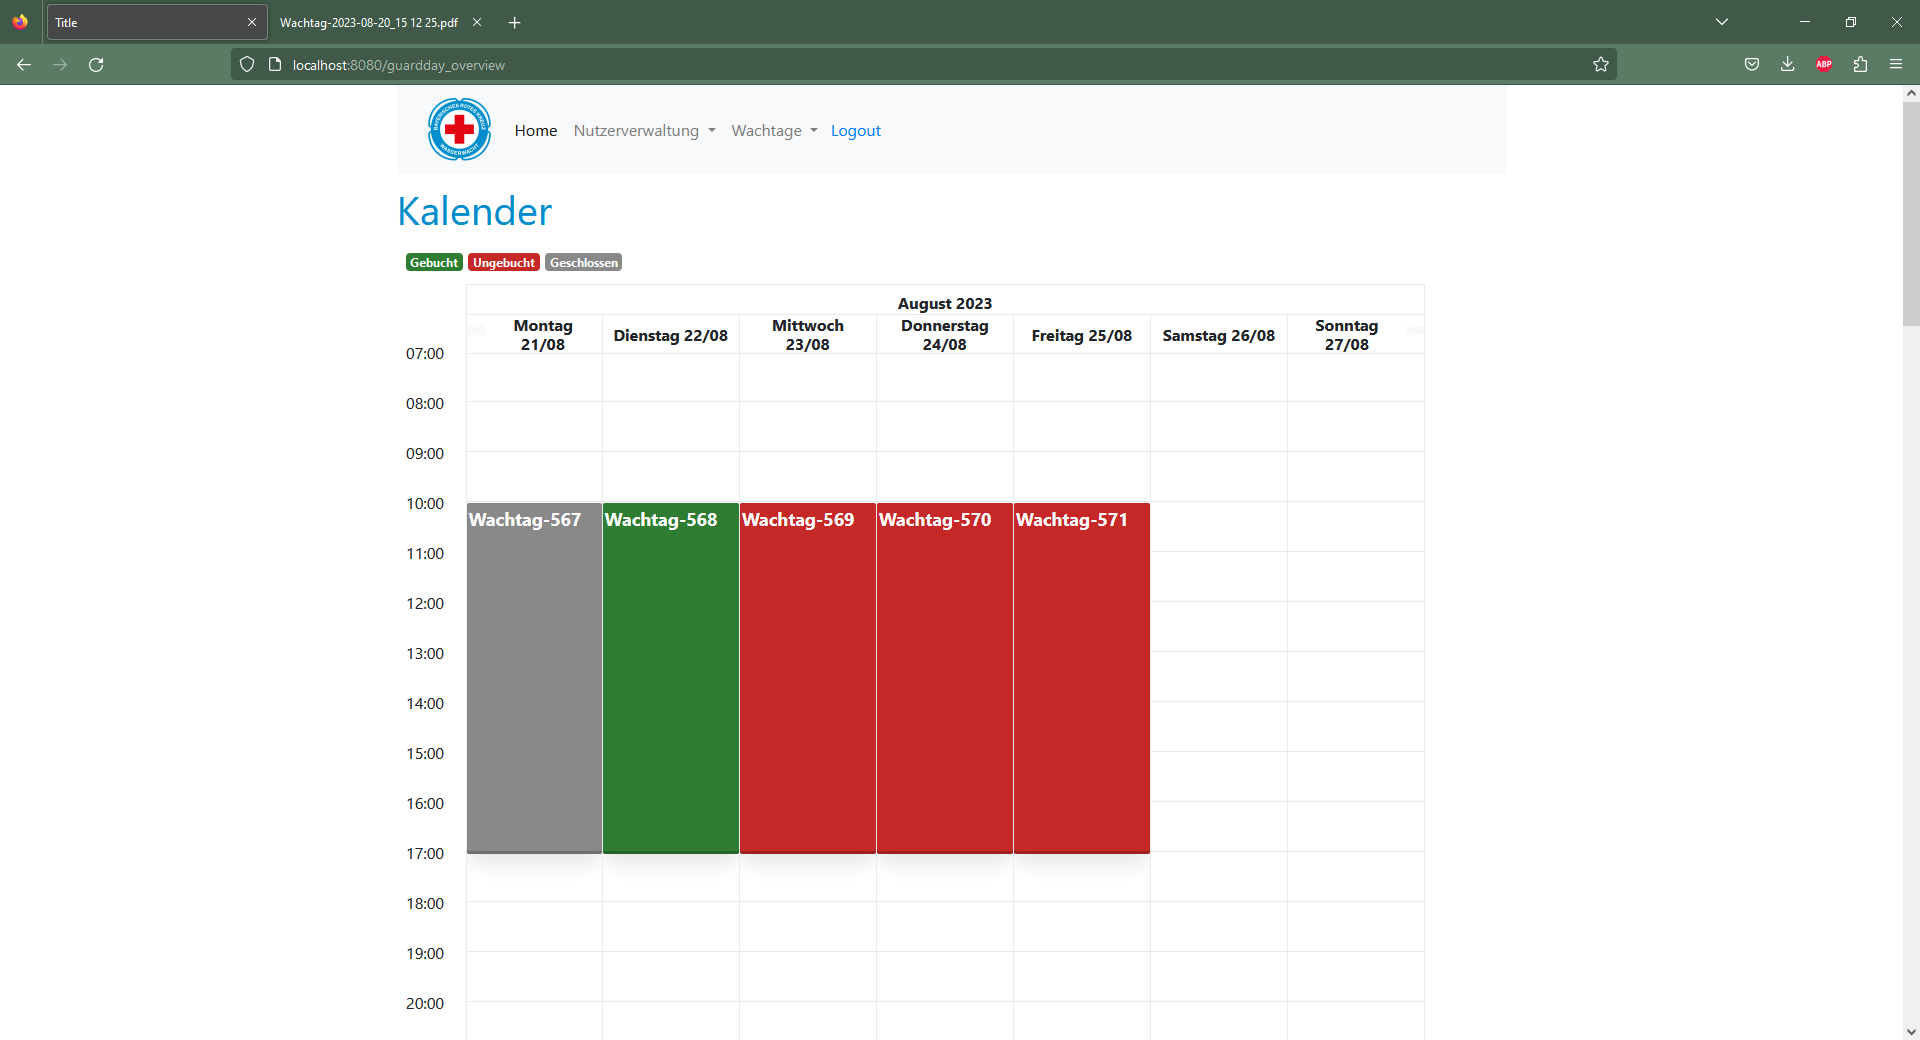
\includegraphics[width=0.7\linewidth]{Anlagen/Anwendung/7UebersichtGebucht.png}
    \caption{Wachtag\"ubersicht}
  \label{fig:anwendung-wachubersicht}
\end{figure}

\subsection {Wachplandurchführung}

Auf der Seite des jeweiligen Wachplans $(siehe~\ref{fig:anwendung-wachtagunbefuellt})$ befindet sich oben zun\"achst das geplante Datum und die geplanten Start- und Endzeitpunkte des Wachtages. Rechts daneben befindet sich die Anzeige der aktuellen Wetterdaten aus der Wetter-Api, die \"uber eine Grafik verdeutlicht, welche Wetterzust\"ande gerade herrschen. Darunter befindet sich ein Eingabefeld der gemessenen Wassertemperatur. Die Eingabe ist jedoch erst m\"oglich, wenn der Wachtag gestartet wurde. \\
Als n\"achstes findet man die Tabellen mit den gebuchten Helfern und den anwesenden Helfern. Diese k\"onnen hinzugef\"ugt werden, indem entweder aus der Dropdown-Liste \glqq Nutzer w\"ahlen\grqq{} registrierte Nutzer ausgew\"ahlt werden, oder in dem Eingabefeld \glqq Nutzer Eingabe\grqq{} als Helfer erfasst werden. Wenn ein Wachtag noch nicht begonnen hat, wird ein Helfer als gebuchter Helfer gespeichert $(siehe~\ref{fig:anwendung-wachtaggebucht})$. Hier besteht noch die M\"oglichkeit, sich wieder aus einem Wachplan, \"uber das M\"ulltonnen-Icon neben dem Namen, auszutragen. Sobald ein Wachtag begonnen hat, werden die so eingegebenen Nutzer als anwesende Helfer gepeichert. \\
Darunter befinden sich noch die Buttons \glqq Wachbeginn\grqq{}, um einen Wachtag zu starten, sowie der Button \glqq Anmeldung ILS\grqq{}, um eine An- und Abmeldung in der ILS zu dokumentieren. Der Button \glqq Anmeldung ILS\grqq{} ist allerdings auch erst aktiv, wenn der Wachtag gestartet wurde. \\
Zuletzt findet man noch ein Textfeld, \"uber das man Eintr\"age in das Wachbuch schreiben kann. Hier besteht die M\"oglichkeit ein registriertes Mitglied aus der Liste \glqq Nutzer w\"ahlen\grqq{} auszuw\"ahlen. Diese Person wird dann als Verfasser des Wachbucheintrags gespeichert. Wenn man keinen Nutzer aus der Liste ausw\"ahlt, gilt der eingeloggte Anwender als Verfasser der Nachricht. In der darunterliegenden Tabelle sind die einzelnen Wachbucheintr\"age mit Zeitstempel und Nutzer chronologisch abgelegt.

\begin{figure}[H]
  \centering
    \includegraphics[width=0.7\linewidth]{Anlagen/Anwendung/8WachtagUnbefuellt.png}
    \caption{Wachtag Durchf\"uhrung}
  \label{fig:anwendung-wachtagunbefuellt}
\end{figure}

\begin{figure}[H]
  \centering
    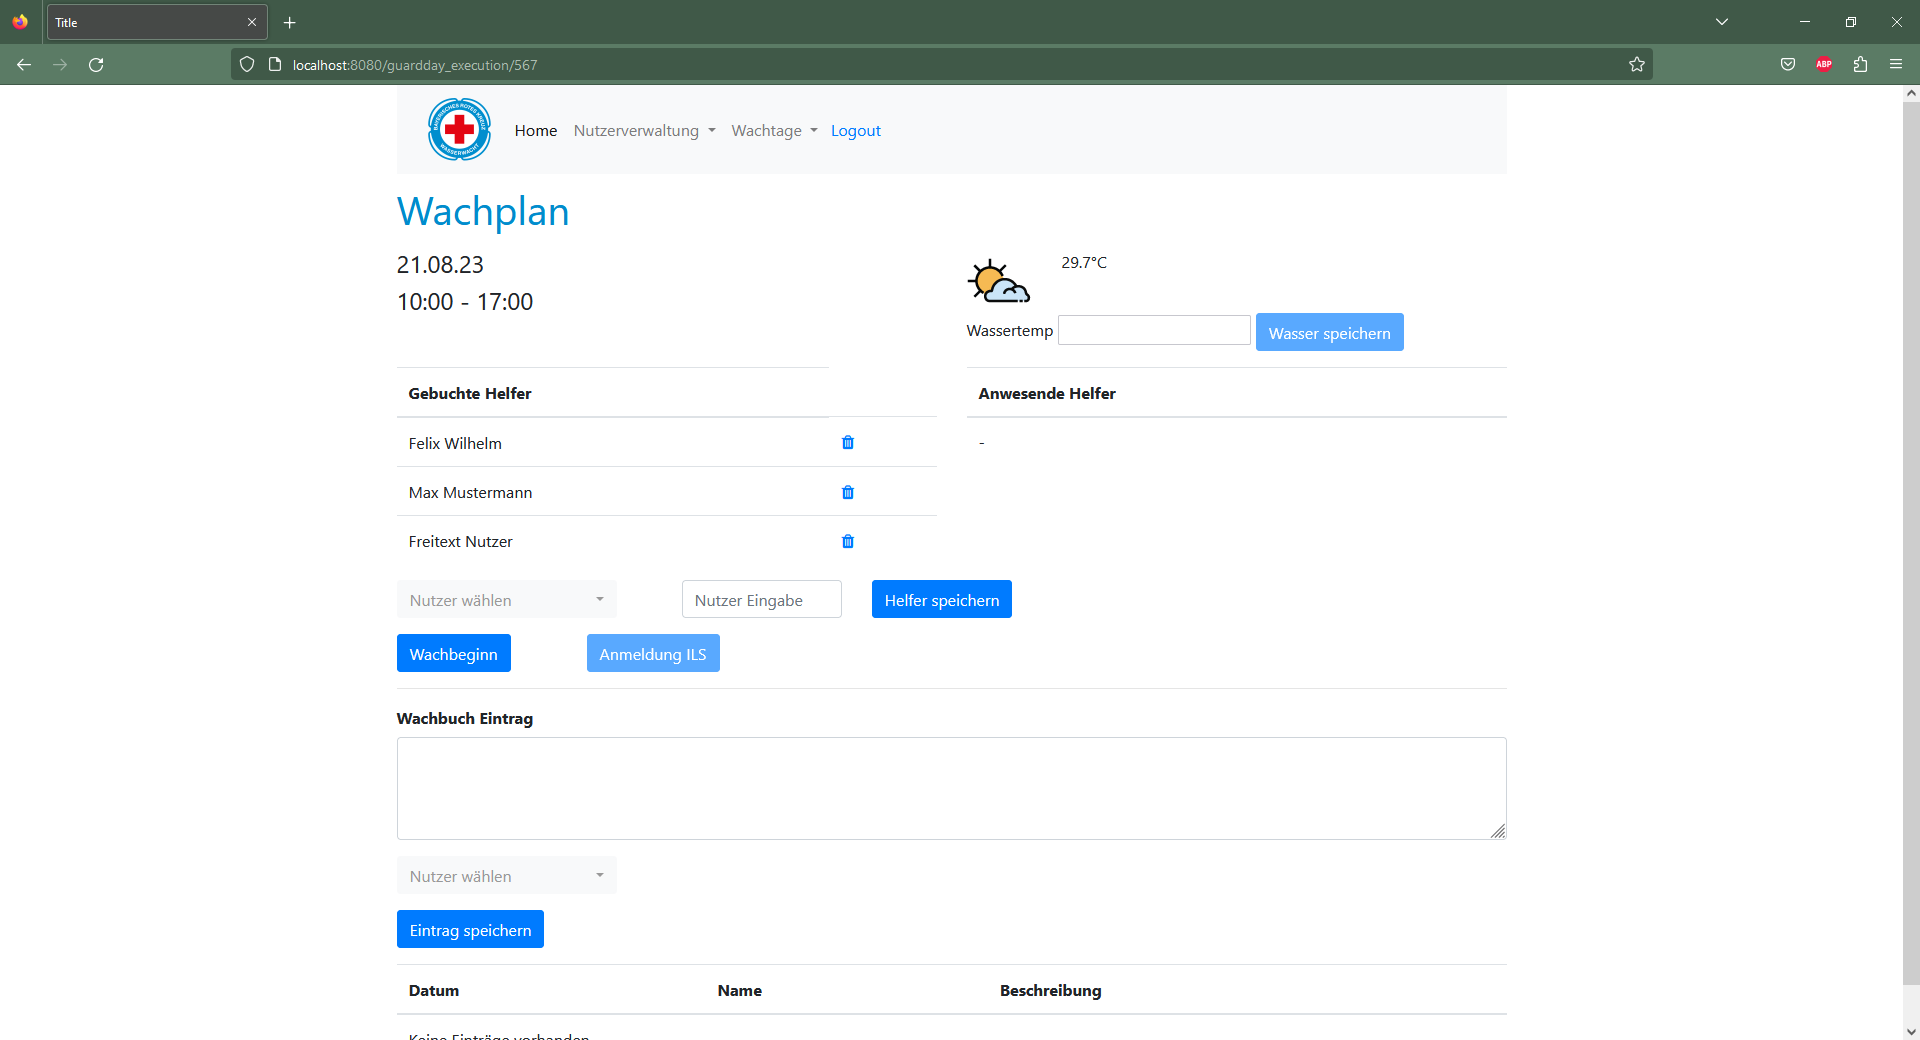
\includegraphics[width=0.7\linewidth]{Anlagen/Anwendung/8-1WachtagNutzerGebucht.png}
    \caption{Wachtag mit gebuchten Helfern}
  \label{fig:anwendung-wachtaggebucht}
\end{figure}

Sobald man einen Wachtag, \"uber einen Klick auf \glqq Wachbeginn\grqq{}, startet, wird der erste Eintrag in das Wachbuch geschrieben um den Wachbeginn zu dokumentieren. \\
In der Liste der gebuchten Helfer wird das Icon der M\"ulltonne entfernt, da man sich nach Wachstart nicht mehr aus dem Plan austragen kann. Stattdessen erscheint an der Stelle jetzt ein Pfeil-Icon. Wird dieses gedr\"uckt, kann man den ausgew\"ahlten Nutzer in die Liste der anwesenden Helfer \"ubertragen. Dies erm\"oglicht es den Mitgliedern, sich schnell f\"ur den Wachtdienst anzumelden. \\
Wenn sich ein Nutzer nach Wachstart f\"ur den Wachdienst anmeldet, wird ein Eintrag in das Wachbuch geschrieben um den Wachbeginn zu dokumentieren. Ein anwesender Helfer kann sich vom Dienst abmelden, indem er das M\"ulltonnen Icon neben seinem Namen dr\"uckt. Dadurch wird auch wieder ein Eintrag generiert, um das Wachende festzuhalten $(siehe~\ref{fig:anwendung-wachtaganwesend})$. \\
Zus\"atzlich ist es jetzt m\"oglich Wassertemperaturen, \"uber das Eingabefeld oben, zu dokumentieren. Bet\"atigt man den Button \glqq Wasser speichern\grqq{}, wird ein Eintrag in das Wachbuch geschrieben. \\

\begin{figure}[H]
  \centering
    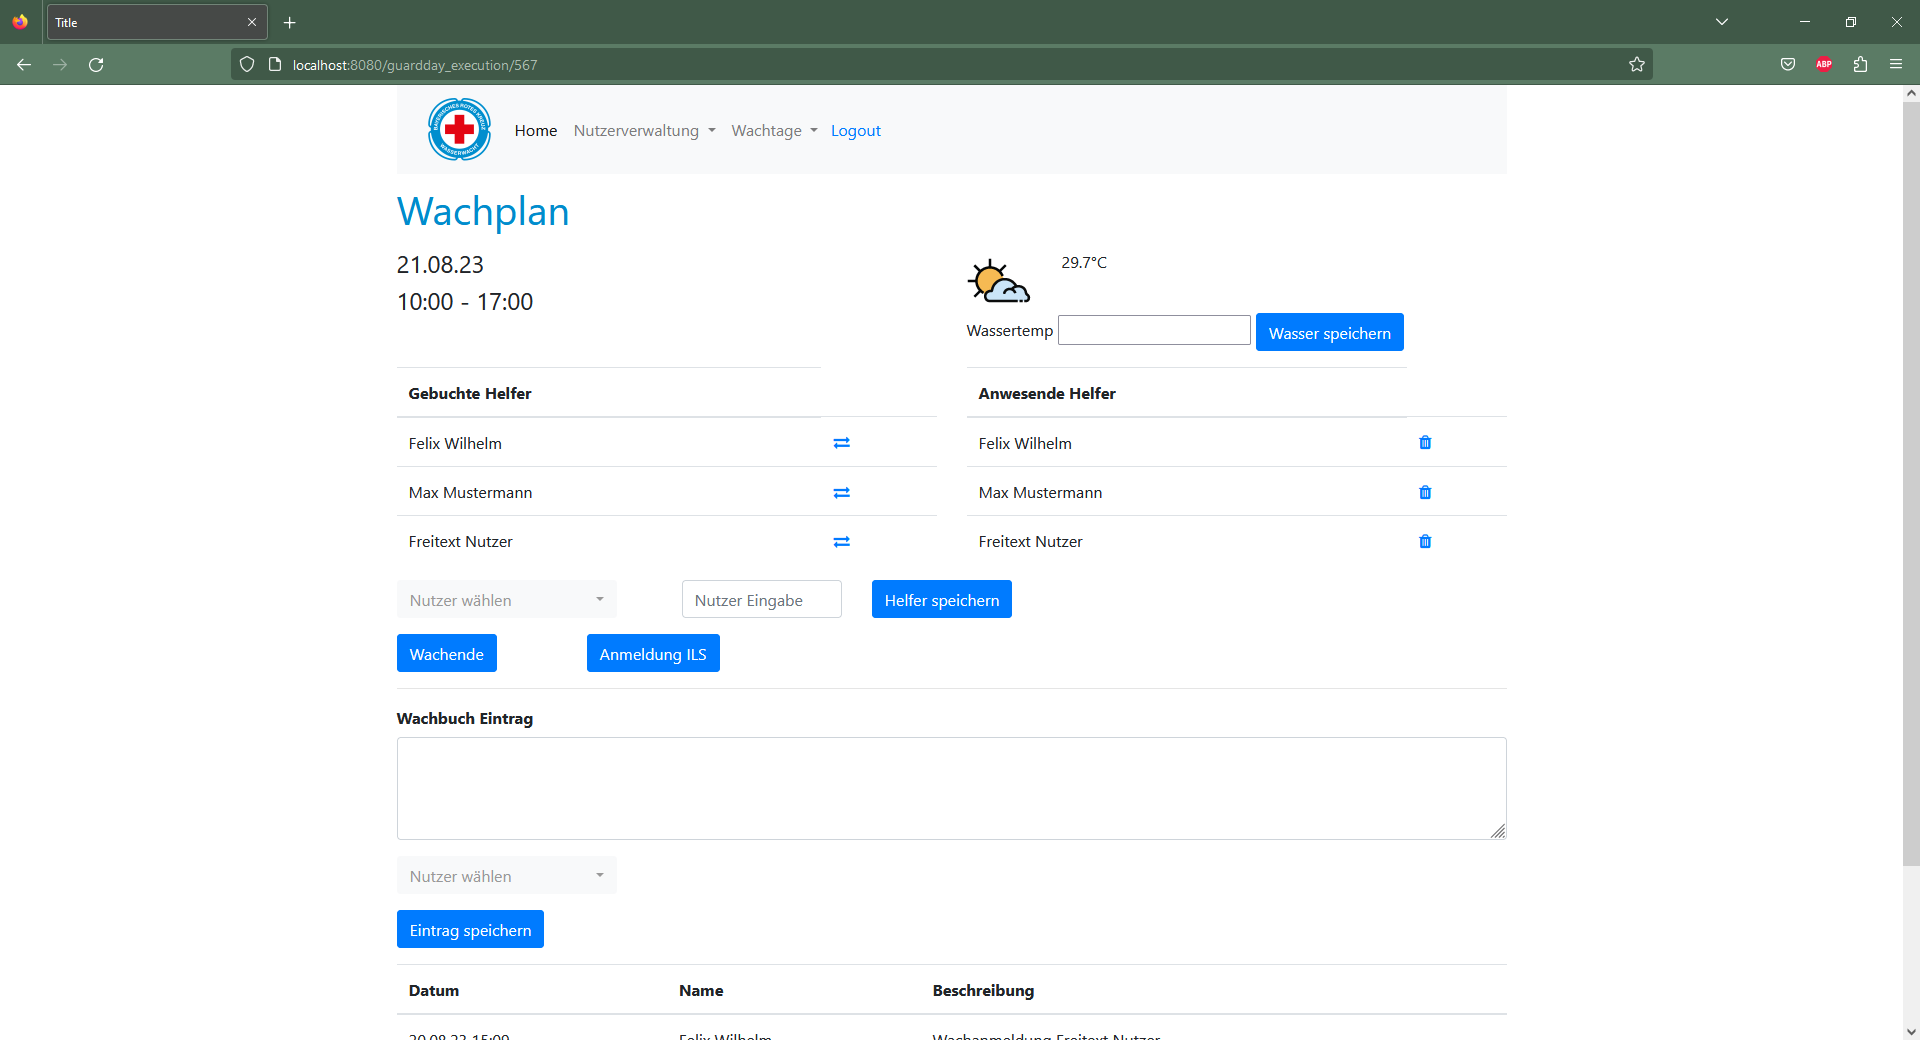
\includegraphics[width=0.7\linewidth]{Anlagen/Anwendung/8-3WachtagAnwesendeNutzer.png}
    \caption{Wachtag mit anwesenden Helfern}
  \label{fig:anwendung-wachtaganwesend}
\end{figure}

Die Wetterdaten werden automatisch in das Wachbuch geschrieben. Dies wurde umgesetzt, indem ein asynchroner Methodenaufruf abgesetzt wird. Dies bedeutet, dass die Methode aufgerufen wird, jedoch nicht auf das Ergebnis gewartet werden muss. \\
In der Methode wird zun\"achst eine konfigurierte Zeit lang gewartet, bevor der Wachtag gelesen wird. Danach wird eine while-Schleife begonnen, die so lange l\"auft, bis der Wachtag beendet wurde. Innerhalb der Schleife werden dann die aktuellen Wetterdaten aus der Api gelesen und als Wachbucheintrag dem jeweiligen Wachtag beigef\"ugt und gespeichert. Danach wird wieder eine konfigurierte Zeit gewartet, bevor der Wachtag erneut gelesen wird. Somit kann die Bedingung der while-Schleife erneut abgepr\"uft werden. 

\begin{figure}[H]
  \centering
    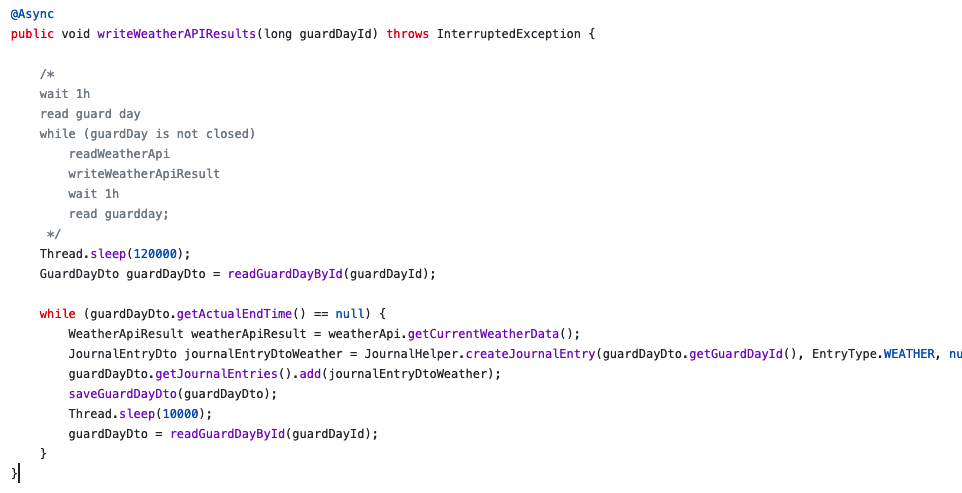
\includegraphics[width=0.7\linewidth]{Anlagen/Code/weatherApiAsync.png}
    \caption{Auszug aus GuardDayService.java - Automatische Speicherung der Wetterdaten}
  \label{fig:code-weatherapi}
\end{figure}
 
Nach Beenden des Wachtages durch Klick auf \glqq Wachende\grqq{} werden alle noch anwesenden Helfer abgemeldet. Au{\ss}erdem wird das Wachende im Wachbuch festgehalten. Alle Buttons f\"ur diesen Wachtag, bis auf das Wachbuch, werden deaktiviert, da ein beendeter Wachtag nicht mehr bearbeitet werden darf $(siehe~\ref{fig:anwendung-wachende})$. Nach Wachende ist es immer noch möglich Einträge für das Wachbuch zu verfassen.\\
Einen beendeten Wachtag kann man sich im Nachhinein noch ansehen. So kann man \"uber das Wachbuch den Verlauf des Wachtages nachvollziehen $(siehe~\ref{fig:anwendung-wachbuch})$.

\begin{figure}[H]
  \centering
    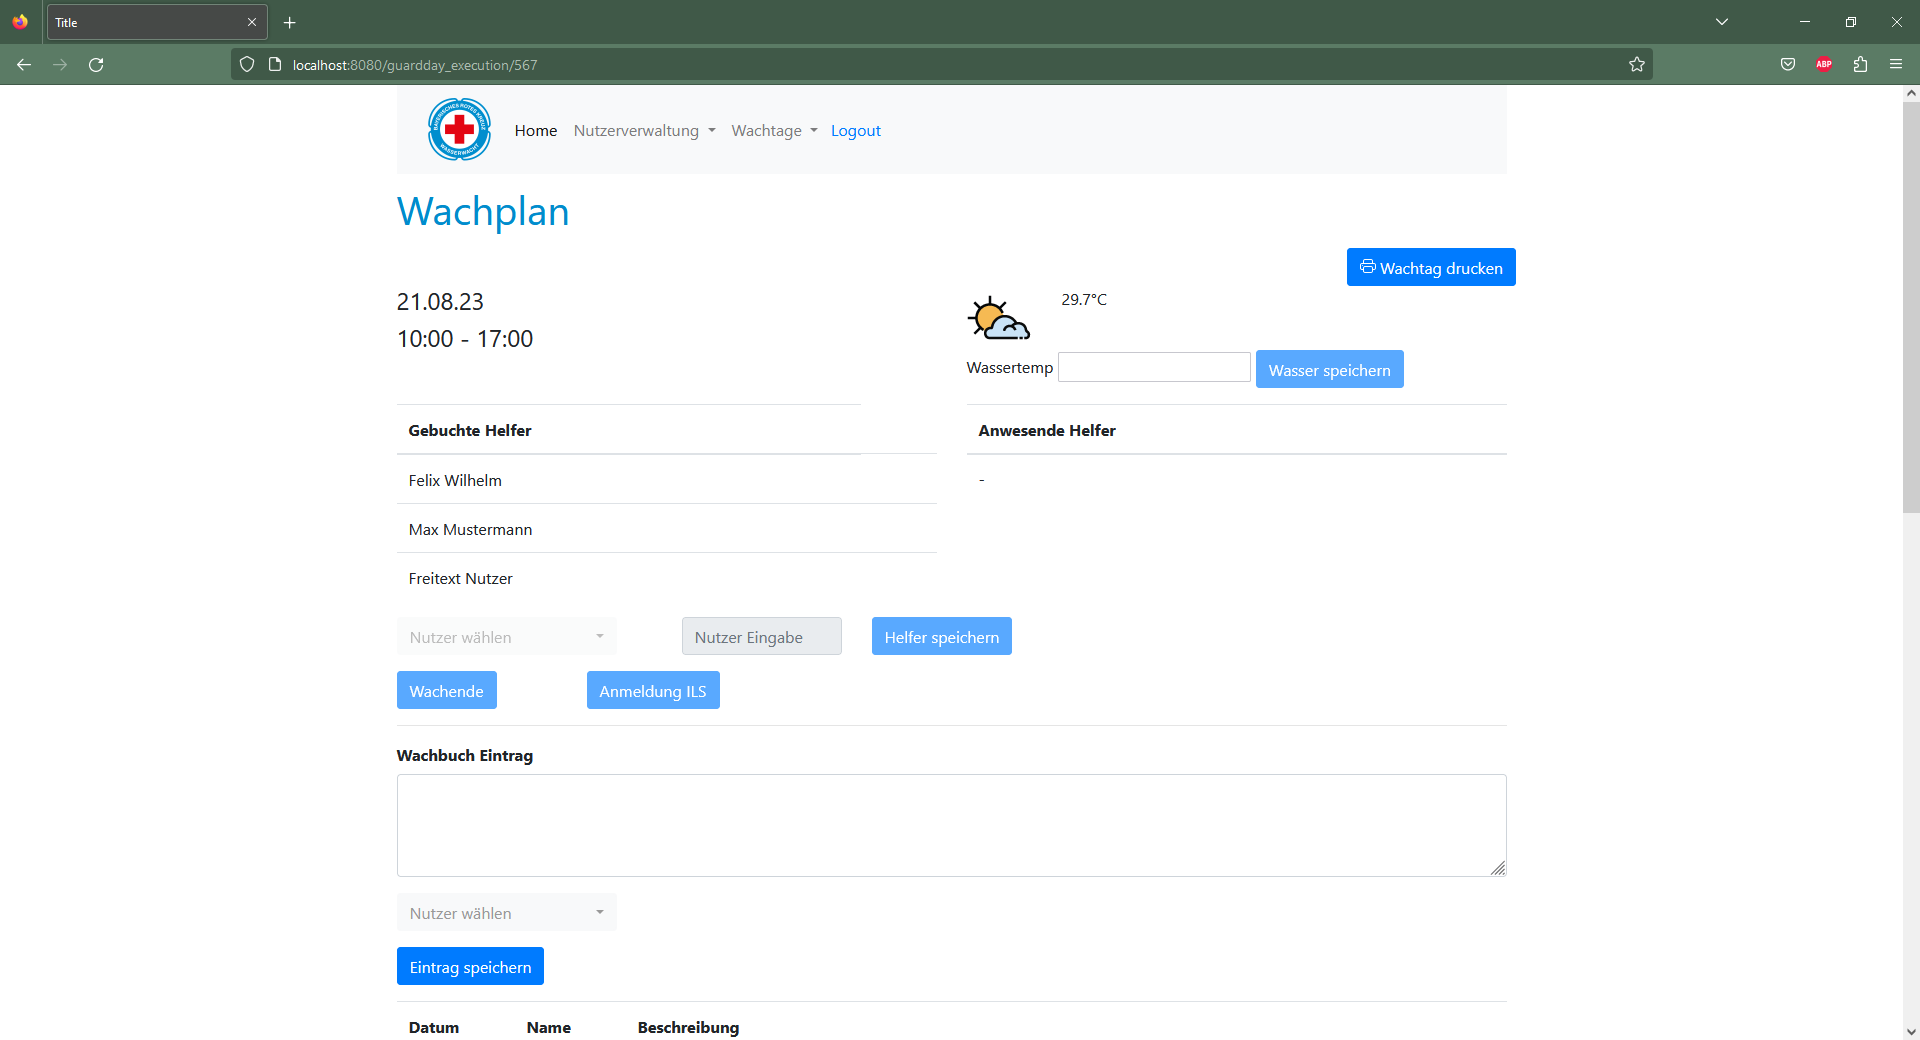
\includegraphics[width=0.7\linewidth]{Anlagen/Anwendung/8-5WachtagWachende.png}
    \caption{Wachende}
  \label{fig:anwendung-wachende}
\end{figure}

\begin{figure}[H]
  \centering
    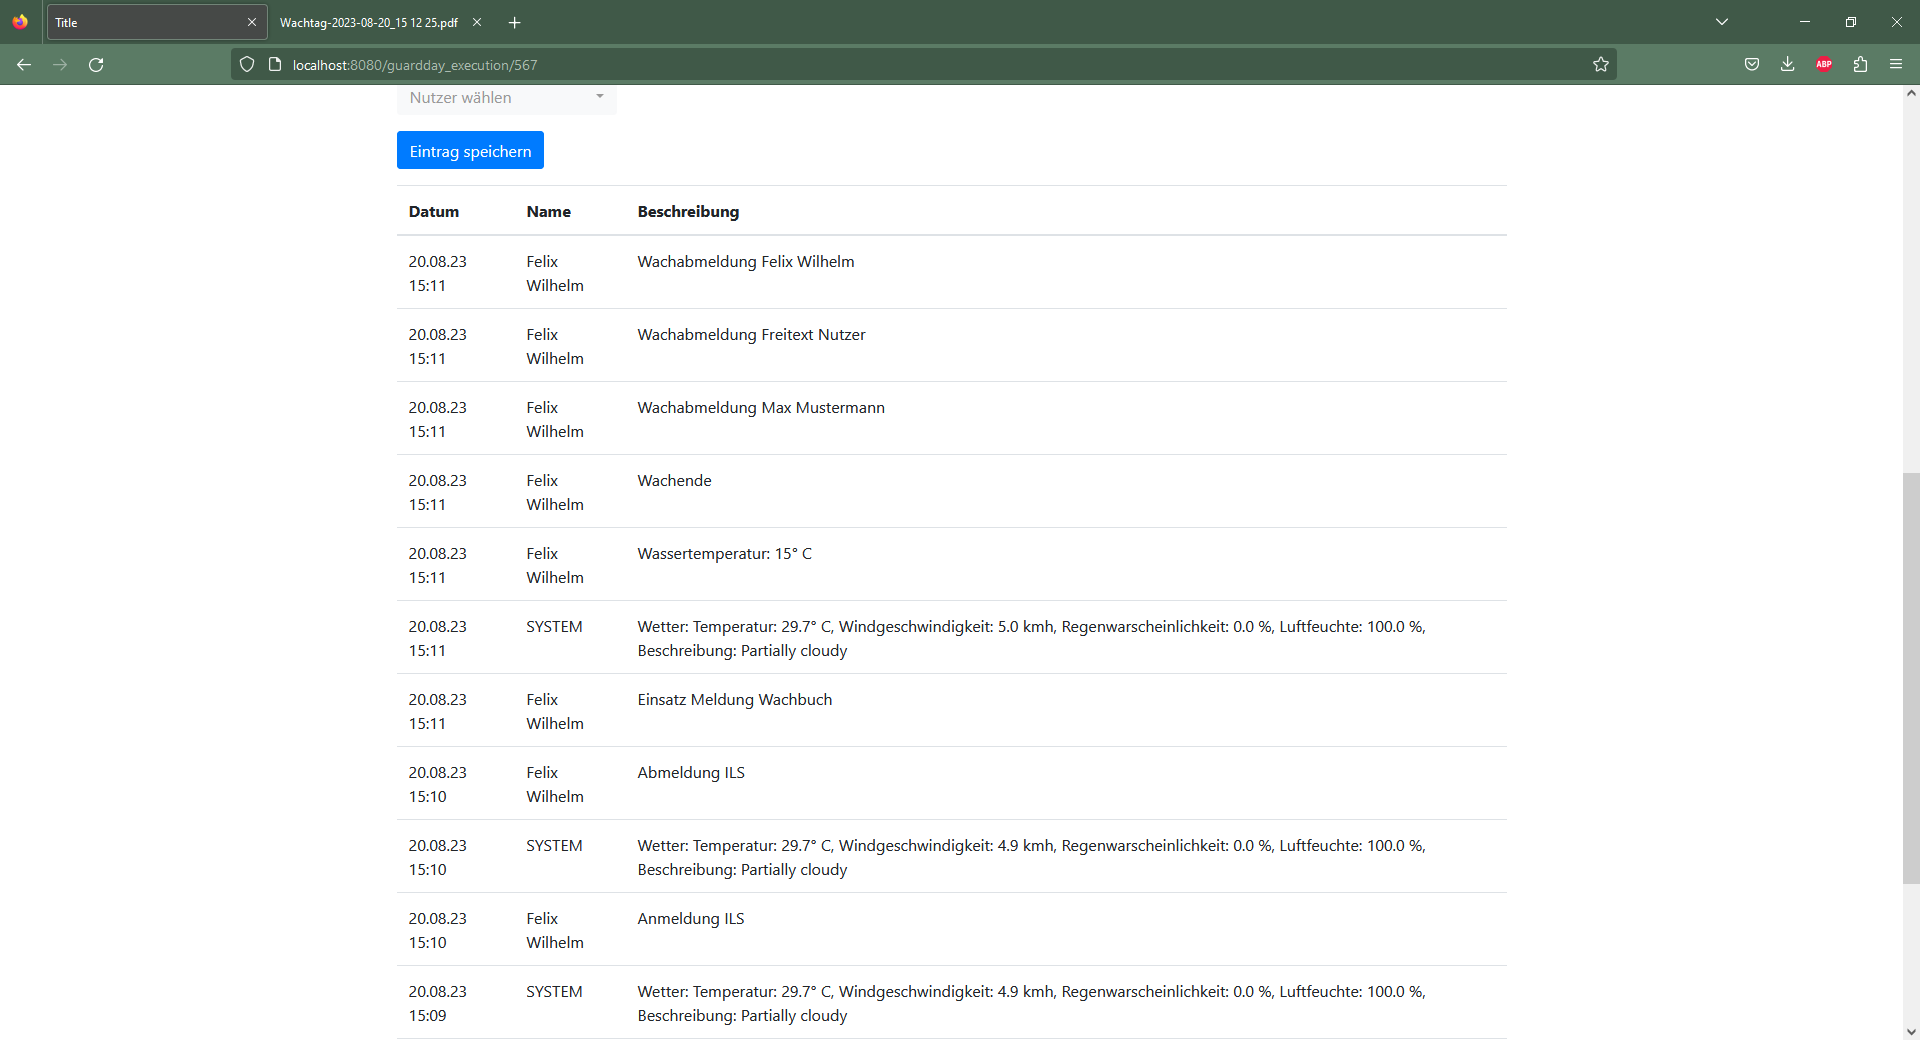
\includegraphics[width=0.7\linewidth]{Anlagen/Anwendung/8-6WachtagWachbuchLog.png}
    \caption{Wachbuch}
  \label{fig:anwendung-wachbuch}
\end{figure}


\subsection{Druckfunktionalität}

Nach Ende eines Wachtages besteht die M\"oglichkeit, sich ein PDF aus den Wachbucheintr\"agen zu generieren. Dazu wird ein Button oben rechts \glqq Wachtag drucken\grqq{} $(siehe~\ref{fig:anwendung-wachende})$ eingeblendet. Leitungskr\"afte haben so die M\"oglichkeit einen detaillierten Verlauf des Wachtages mit allen Geschehnissen abzulegen (siehe \ref{fig:wachtagexport}). \\
Umgesetzt wurde die Druckfunktionalit\"at mittels der Open-Source Java-Library OpenPDF von LibrePDF. Diese erm\"oglicht es \"uber Java Code eine PDF-Datei zu erzeugen.\\

%\section{Umsetzung der Webanwendung anhand von Best Practises}


%%%%%%%%%%%%%%%%%%%%%%%%%%%%%%%%%%%%
%
% Kapitel 6
%
%%%%%%%%%%%%%%%%%%%%%%%%%%%%%%%%%%%%

%\renewcommand{\cleardoublepage}{}
\newpage
\chapter{Evaluation}

Um sicherzustellen, dass die Website den Anforderungen der Wasserwacht entspricht, wird im Folgenden eine Evaluierung durchgeführt. Dies geschieht zunächst mit Nutzertest und Befragung von Wasserwachtmitgliedern. Dadurch soll die Praxistauglichkeit und Effektivität der Webanwendung bewertet werden. Außerdem werden noch \glqq Klickmetriken\grqq{} betrachtet, für die zwei Haupt-Anwendungsfälle Wachplanerstellung und Wachplandurchführung. Abschließend wird daraus ein Fazit gezogen und auf Verbesserungspotentiale eingegangen. 

\section{Nutzertests}

Für die Nutzertests wurden drei unabhängige Personen herangezogen. Diesen wurde zunächst der Prozess der Wachplanung der Wasserwacht erläutert und anhand der aktuellen Papierform (siehe Anhang ~\ref{fig:wachbuchpapier}) aufgezeigt. Im nächsten Schritt wurde ihnen die Webanwendung präsentiert und die einzelnen Prozessschritte erläutert, die zur Wachplanung und Durchführung gehören. \\
Anschließend wurde ihnen ein Bewertungsbogen vorgelegt mit 11 Fragen, die auf die Benutzerfreundlichkeit und Praxistauglichkeit der Anwendung abzielen. Diese 11 Fragen waren mit Punkten von 1 bis 5 zu bewerten, wobei 1 sehr schlecht entspricht und 5 sehr gut. Zusätzlich gab es noch zwei offene Fragen, um Verbesserungspotentiale und Kritik abzufragen. \\
Aus den Bewertungsfragen wird anschließend ein Score berechnet, der den Durchschnitt über alle Fragen abbildet. Ziel ist es hier über den Mittelwert von 33 zu kommen. Dieser würde sich ergeben wenn alle Fragen mit 3 bewertet würden. \\
Wird dieses Ziel erreicht, wird von einer benutzerfreundlichen Website ausgegangen.

\subsection{Fragenkatalog}
\subsubsection{Bewertungsfragen}
Zunächst wurden Fragen definiert, die auf die generelle Nutzerzufriedenheit mit der Website abzielen. Dazu wird der Nutzer zu Design, Navigation, Verständlichkeit und Zugänglichkeit von Informationen befragt.

1. Wie zufrieden waren Sie mit dem Design und Layout der Website?\\
2. Wie leicht war es für Sie, die Informationen zu finden, nach denen Sie gesucht haben?\\
3. Wie einfach war es für Sie, sich auf der Website zu orientieren?\\
4. Wie benutzerfreundlich fanden Sie die Navigation auf der Website?\\
5. Wie gut funktionieren die interaktiven Funktionen auf der Website (z.B. Suchfeld, Formulare, ...) ?\\
6. Wie verständlich sind die Hinweise und Anweisungen auf der Website?

Im nächsten Teil, zielen die Fragen auf die Zufriedenheit mit der Umsetzung der Prozesse ab. Dadurch soll man erkennen, ob durch die digitalen Prozesse ein Mehrwert entstanden ist im Vergleich zum analogen Vorgehen.

7. Wie einfach ist es einen Wachplan anzulegen?\\
8. Wie einfach ist es einen Wachplan durchzuführen? \\
9. Wie schnell war der digitale Verwaltungsprozess im Vergleich zum analogen Verfahren? \\
10. Wie zufrieden sind Sie mit dem Ergebnis des digitalen Verwaltungsprozesses im Vergleich zum analogen Verfahren? \\
11. Wie wahrscheinlich ist es, dass Sie die digitale Version des Verwaltungsprozesses im Vergleich zur analogen Version nutzen möchten?

\subsubsection{Offene Fragen}
1. Wie könnte man die Website noch verbessern? \\
2. Gibt es noch abschließendes Feedback / Kritik?\\

\subsection{Ergebnisse}
In Tabelle \ref{tab:survey} sind die Ergebnisse der einzelnen Fragen aufgezeigt. Als Ergebnis wird immer der durchschnittliche Score aus den 3 Umfrageteilnehmern genommen. \\
Addiert man diese Ergebniswerte auf, erhält man einen Score von 49,34. Somit wurde das Ziel einer benutzerfreundlichen Webanwendung erreicht.

\begin{table}[ht]
\centering
\caption{Ergebnisse der Nutzerumfrage}
\label{tab:survey}
\begin{tabular}{|c|c|}
\hline
Frage & Ergebnis (Durchschnitt) \\
\hline
1 & 4\\
2 & 4,67\\
3 & 4,67\\
4 & 4,33\\
5 & 4,67\\
6 & 4,33\\
7 & 5\\
8 & 3,67\\
9 & 5 \\
10 & 4,67 \\
11 & 4,33 \\
\hline
\end{tabular}
\end{table}

Für die offenen Fragen gab es folgende Antworten: \\
\textbf{Wie könnte man die Website noch verbessern?} \\
1. Die Farbgebung ist etwas eintönig, was allerdings Sinn macht, da es den Farben des Wasserwacht Logos folgt. \\
2. Design eher monoton, Buttons heben sich nicht gut hervor, Abgrenzung schwierig. 

\textbf{Gibt es noch abschließendes Feedback / Kritik?} \\
1. Sehr übersichtlich und einfach gehalten, dass einzige was fehlt ist die Anzahl der Schwimmer, Boote etc. am aktuellen Tag in der Übersicht. \\
2. Die Website ist aüßerst übersichtlich, mit Details an der richtigen Stelle. Die Durchführung verschiedener Aktionen ist logisch abgebildet, was die Benutzung angenehm und einfach macht. Äußerst hervorzuheben ist die Zwei-Phasen Authentifizierung zum Schutz der Daten. \\
3. Druckfunktionalität ist gut, alle Informationen können per PDF archiviert oder versendet werden. Sehr übersichtlich. 

\subsection{Diskussion}
Grundsätzlich kann man sehen, dass in der Umfrage positive Ergebnisse bzgl der Website erfasst wurden. Sowohl im ersten Fragenteil zur Benutzerfreundlichkeit, als auch im zweiten Fragenteil zur Prozess-Zufriedenheit konnten hohe Werte erzielt werden. \\  
Dadurch lässt sich feststellen, dass auch Personen ohne fachliche Expertise sich einfach auf der Website zurecht finden. Die Website ist sehr schlicht aufgebaut, wodurch die Personen die Prozesse der Wachplanung und Wachdurchführung sehr schnell verstanden haben. Dies spiegelt sich auch in den offenen Fragen wieder, in denen die Übersichtlichkeit gelobt wird. \\ 
Ein weiterer Punkt aus den offenen Fragen bemängelt das Fehlen eines digitalen Einsatztagebuchs. Dieses kann man am aktuellen Wachbuch in Papierform sehen und beinhaltet verschiedene Einsatzdaten, wie zum Beispiel wie viele Einsätze mit Boot abgeschlossen wurden. \\
Das Einsatztagebuch ist auch im initialen Entwurf der Plansoftware (s.h. \ref{fig:initial}) zu sehen. Aus zeitlichen Gründen wurde sich in dieser Bachelorarbeit nur mit der Wachplanung und Durchführung befasst. Als Erweiterungsmöglichkeit wäre es aber durchaus wichtig. \\
Weiterhin wird das monotone Design kritisiert bezüglich eintöniger Farbgebung und fehlender Hervorhebung von Formularen. \\
Für die Bachelorarbeit wurde der Fokus eher auf eine korrekte Umsetzung der Prozesse gelegt.  Aus den Umfrageergebnissen zeigt sich aber, dass das Design auch eine wichtige Rolle spielt. Dies kann daher als Verbesserungsmöglichkeit in zukünftiger Weiterentwicklung mit aufgenommen werden.

Obwohl für die Nutzertests eine sehr kleine Personengruppe herangezogen wurde, waren sie dennoch sehr aufschlussreich. Besonders über das offene Feedback ließen sich die unterschiedlichen Vorstellungen verschiedener Personen einfangen. Für einen weiteren Durchlauf wäre eine größere Personengruppe von Vorteil, um weitere Einblicke in die Präferenzen der Nutzer zu erfassen.

\section{Klickmetriken}
Im Folgenden werden Klickmetriken gemessen und analysiert für die zwei Hauptprozesse Wachplanerstellung und Wachplandurchführung. Dazu wird betrachtet, wie viele Klicks man benötigt um zur gewünschten Zielseite zu gelangen. Weiterhin werden dann die Klicks gemessen die für die Durchführung der Prozessschritte benötigt werden.

\subsection{Wachplanerstellung}
Für die Wachplanerstellung wird als Ausgangspunkt die Startseite festgelegt. \\
Um zur Seite der Wachplanerstellung zu gelangen werden zwei Klicks benötigt. Zunächst klickt man in der Navigationsleiste auf \glqq Wachtag Übersicht\grqq{} und dann auf den Unterpunkt \glqq Wachtagerstellung\grqq{}. \\
Für die Anlage eines einzelnen Wachtages werden 4 Klicks benötigt. Diese ergeben sich aus den jeweiligen Eingabefeldern \glqq Datum\grqq{}, \glqq Startzeit\grqq{} und \glqq Endzeit\grqq{} und einem Klick zum speichern. \\
Für die Anlage einer Terminreihe werden 7 - 13 Klicks benötigt. Zunächst muss man auf \glqq Terminreihe anlegen\grqq{} klicken um zur Anlage zu gelangen. Danach werden die Eingabefelder \glqq Startdatum\grqq{}, \glqq Enddatum\grqq{}, \glqq Startzeit\grqq{} und \glqq Endzeit\grqq{} befüllt. Die Auswahl der Tage, an denen ein Wachtag erzeugt werden soll, wurde mit Hilfe von Checkboxen umgesetzt. Daher sind hier 1 - 7 Klicks notwendig. Abschließend muss man die Reihe noch speichern. 

\subsection{Wachplandurchführung}
Für die Durchführung eines Wachtags wird ein einfacher Nutzer verwendet. Als Ausgangspunkt gilt wieder die Startseite. \\
Um zu dem jeweiligen Wachtag zu gelangen werden drei Klicks benötigt. Zunächst klickt man in der Navigationsleiste auf \glqq Wachtagübersicht\grqq{}. Danach wählt man einen Wachtag im Kalender aus und bestätigt die Auswahl in einem sich öffnendem Modal. 

Da die Wachplandurchführung je nach Wachtag unterschiedlich ist und auch nicht in einer Sitzung alle Punkte abgearbeitet werden, wird im Folgenden auf die Klicks der einzelnen Prozessschritte eingegangen.

\subsubsection{Einbuchung}
Um sich für einen noch nicht gestarteten Wachtag einzubuchen klickt man auf die Liste \glqq Nutzer wählen\grqq{} und wählt den entsprechenden Nutzer aus. Durch Klick auf \glqq Helfer speichern\grqq{} wird der Nutzer für den Wachtag hinterlegt. \\
Somit ergeben sich drei Klicks.

\subsubsection{Wachbeginn}
Für den Wachbeginn werden zwei Klicks benötigt. Zunächst startet man den Wachtag durch Klick auf \glqq Endzeit\grqq{Wachbeginn}. Danach kann man in der Liste der gebuchten Helfer durch Klick auf das Pfeil-Icon einen Nutzer anmelden.

\subsubsection{Wassertemperatur messen}
Um die Wassertemperatur zu dokumentieren werden zwei Klicks benötigt. Zunächst klickt man in das Eingabefeld der Wassertemperatur. Anschließend wird der Eintrag gespeichert.

\subsubsection{An- / Abmeldung ILS}
Für die An- und Abmeldung im ILS werden zwei Klicks benötigt.

\subsubsection{Wachbuch Eintrag}
Um einem Wachbuch Eintrag anzulegen klickt man zunächst in das Eingabefeld \glqq Wachbuch Eintrag\grqq{}. Nach erfassen des Eintrags speichert man das ganze durch Klick auf \glqq Eintrag speichern\grqq{}. Das entpricht zwei Klicks.

\subsection{Interpretation}
Insgesamt kann festgestellt werden dass Nutzer der Website nur geringe Anzahlen an Klicks aufwenden müssen, um ihre gewünschten Ziele zu erreichen. Dies gibt einen Einblick in die minimalistische Gestaltung der Website und ihr schlankes Design. \\ 
Durch das minimalistische Design werden überflüssige und ablenkende Elemente eliminiert, wodurch eine klare und fokussierte Benutzererfahrung entsteht. Dies führt zu einer effizienteren Navigation und Interaktion, da Nutzer weniger Schritte durchlaufen müssen, um Prozesse abzuarbeiten. \\
Die Website ist so gestaltet, dass sie intuitiv und leicht zu bedienen ist. Indem die Anzahl der erforderlichen Klicks minimiert wird, wird der Zugang zu Informationen und Funktionen erleichtert, was besonders für Nutzer mit geringerer technischer Erfahrung von Vorteil ist. 

\section{Verbesserungspotentiale}

\subsubsection{Fehlende Bearbeitungsmöglichkeiten in Profil und Wachplanung}
Derzeit können Benutzer einen einmal erstellten Wachtag nicht löschen oder bearbeiten. Zudem fehlt auch die Bearbeitungsmöglichkeit im Nutzerprofil. \\ 
Hierzu müssen noch die fehlenden Funktionen implementiert werden und durch zusätzliche Schaltflächen oder interaktive Elemente in der Nutzeroberfläche eingebunden werden. Eine solche Erweiterung würde die Benutzerfreundlichkeit erhöhen und den Benutzern mehr Flexibilität bieten.

\subsubsection{Monotones Design} 
Das aktuelle Design der Webanwendung nutzt Standard Bootstrap, was zu einem eher monotonen Erscheinungsbild führt. \\ 
Hier könnte man das Design weiter personalisieren durch Anpassung von Bootstrap-Themen oder Integration von CSS-Stilen, die über die Standardvorlagen hinausgehen. Durch eigene Farbschemata, Schriftarten und Layout Änderungen könnte man das Design so anpassen, dass es genau auf die Wasserwacht zugeschnitten wird.

\subsubsection{Inkonsistentes responsives Design in der Wachplandurchführung}
Die Webanwendung ist auf mobilen Geräten nur eingeschränkt nutzbar, das viele Felder auf der Seite der Wachplandurchführung vorhanden sind. Die Darstellung auf kleineren Bildschirmen wird dabei unübersichtlich. \\
Durch den Einsatz von MediaQueries könnte man hier das Design noch weiter optimieren, um auch den Gebrauch auf mobilen Geräten zu gewährleisten. 

\section{Ausblick auf zukünftige Entwicklungen und mögliche Erweiterungen der Webanwendung}
Die Webanwendung für die Wasserwacht Dingolfing-Landau hat bereits einen bedeutenden Beitrag zur Digitalisierung und Effizienzsteigerung der Wachplanung und -durchführung geleistet. Dennoch bieten sich verschiedene Möglichkeiten zur Weiterentwicklung und Erweiterung, um den sich ändernden Anforderungen und Möglichkeiten gerecht zu werden.

\subsubsection{Integration fehlender Elemente aus dem Planungsmodell}
Aus zeitlichen Gründen wurden manche Punkte aus dem ursprünglichen Entwurf der Anwendung nicht umgesetzt. Die Integration einer detaillierten Übersicht über verschiedene Checks sowie eines digitalen Einsatztagebuchs würde jedoch die Funktionalität der Anwendung erweitern. Dies könnte die Nachverfolgung und Dokumentation von Ausrüstungschecks und spezifischen Ereignissen während der Wache umfassen, was eine wertvolle Ressource für die Analyse und das Reporting darstellt.

\subsubsection{Erweiterung der Nutzerprofile}
Eine wichtige Erweiterung wäre die Möglichkeit für Nutzer, ihre Qualifikationen und Zertifikate in ihren Profilen zu pflegen. Dies würde eine effizientere Zuweisung von Aufgaben ermöglichen, da die Verantwortlichen schnell die geeignetsten Mitglieder für spezifische Einsätze identifizieren können.

\subsubsection{Integration mit weiteren Systemen}
Die Interoperabilität mit anderen digitalen Systemen der Wasserwacht könnte die Effizienz weiter steigern. Beispielsweise könnte eine Verbindung mit internen Kommunikationssystemen oder Datenbanken die Koordination und Informationsverteilung verbessern.

\subsubsection{Datenschutz und Sicherheit}
Der Datenschutz ist ein kritischer Aspekt, der in der ursprünglichen Implementierung nicht ausreichend berücksichtigt wurde. Es ist notwendig, die Anwendung in Übereinstimmung mit den Datenschutzgesetzen, wie der DSGVO, zu überarbeiten. Dies beinhaltet die Implementierung von Funktionen zur Datensicherheit und die Gewährleistung der Transparenz in der Datenverarbeitung.

\subsubsection{Technische Infrastruktur und Sicherheit}
Für eine verbesserte Performance und Zuverlässigkeit sollte die Anwendung auf einem dedizierten Server installiert werden. Zusätzlich ist ein robustes System zur Datensicherung und -wiederherstellung von entscheidender Bedeutung, um Datenverlust zu vermeiden und die Kontinuität des Betriebs zu gewährleisten.

\subsubsection{Fazit}
Diese potenziellen Erweiterungen und Entwicklungen würden nicht nur die Funktionalität der Webanwendung erhöhen, sondern auch die allgemeine Effizienz und Effektivität der Operations- und Planungsprozesse der Wasserwacht Dingolfing-Landau verbessern. Durch kontinuierliche Anpassungen und Verbesserungen kann die Anwendung den sich wandelnden Bedürfnissen der Nutzer gerecht werden und einen wesentlichen Beitrag zur digitalen Transformation der Wasserwacht leisten.


%%%%%%%%%%%%%%%%%%%%%%%%%%%%%%%%%%%%
%
% Kapitel 7
%
%%%%%%%%%%%%%%%%%%%%%%%%%%%%%%%%%%%%

%\renewcommand{\cleardoublepage}{}
%\chapter{Ergebnisse und Diskussion}

%\section{Zusammenfassung der Ergebnisse}

%\section{Diskussion der Erkenntnisse im Kontext der Zielsetzung der Arbeit}

%\section{Ausblick auf zukünftige Entwicklungen und mögliche Erweiterungen der Webanwendung}

%%%%%%%%%%%%%%%%%%%%%%%%%%%%%%%%%%%%
%
% Kapitel 8
%
%%%%%%%%%%%%%%%%%%%%%%%%%%%%%%%%%%%%

\newpage

\renewcommand{\cleardoublepage}{}
\chapter{Fazit}

\section{Zusammenfassung der Arbeit}
Ziel dieser Arbeit war es, die Herausforderungen der Wachplanerstellung der Wasserwacht zu indentifizieren und durch den Einsatz von IT-Lösungen zu bewältigen. \\ 
In Kapitel 2 wurden die theoretischen Hintergründe dieser Arbeit aufgegriffen. Es wurde zum einen die Wasserwacht allgemein beschrieben, sowie auf Herausforderungen bei der Wachplanerstellung eingegangen. \\
In Kapitel 3 wurden die genauen Anforderungen an die Webanwendung festgemacht. Dazu wurden in mehreren Treffen mit Wasserwachtmitgliedern die Nutzergruppen festgelegt und die Prozesse der Wachplanung und Wachbuchführung festgehalten. Mit Hilfe von Mockups wurden die Ergebnisse daraus veranschaulicht. So hatte man bereits im frühen Entwicklungsstadium einen Überblick, wie die Webanwendung aussehen wird. \\
Nachfolgend wurden die geeigneten Technologien zur Umsetzung der Website ausgewählt. Diese wurden anhand von persönlicher Erfahrung, sowie Eignung für das Projekt ermittelt. In Kapitel 4 werden diese näher beschrieben. \\
In Kapitel 5 wird dann näher auf die Implementierung eingangen. Zunächst wird das zu Grunde liegende Datenmodell anhand eines UML Diagramms beschrieben. Daraufhin werden die umgesetzten Funktionalitäten und Prozesse dargestellt. \\
Abschließend wurde noch eine Evaluation durchgeführt. Zum einen wurde ein Nutzertest durchgeführt, wobei einer Personengruppe die Webanwendung vorgestellt wurde und im Anschluss ein Bewertungsbogen ausgefüllt wurde. Weiterhin wurden auch noch Klickmetriken innerhalb der Website erfasst und analysiert. \\ 
Daraus lies sich ein gutes Feedback für die Anwendung ziehen sowie Problemstellen identifizieren.

\section{Schlussfolgerungen und Handlungsempfehlungen}
Mit dieser Bachelorarbeit wurde aufgezeigt, dass man analoge Verwaltungsprozesse sehrwohl als digitale Lösungen abbilden kann. Dazu bedarf es einer intensiven Planung mit fachlich vertrauten Personen.\\ 
Um sicherzustellen, dass diese Prozesse zur Zufriedenheit der Nutzer korrekt umgesetzt werden, braucht es eine Testphase. Im Kontext der Webanwendung für die Wasserwacht, wäre die Empfehlung das System auf einem den Mitgliedern zugänglichem Server zu installieren. Über eine längere Testphase könnte man so mit dem System arbeiten und vertraut werden. Dadurch könnte man Erfahrungen sammeln und auch mögliche Schwachstellen weiter identifizieren.\\ 
Weiterhin wäre es wichtig auf eine Datensicherung zu achten. Um sicher zu gehen, dass die erfassten Daten der Wachtage nicht verloren gehen, könnte man regelmäßig Datenabzüge machen und entweder über verschiedene RAID-Systeme oder über Cloudanbieter sicher speichern. \\ 
So kann sichergestellt werden, dass die Digitalisierung von Verwaltungsprozessen optimal verläuft.


%%%%%%%%%%%%%%%%%%%%%%%%%%%%%%%%%%%%
%
% Anlagen
%
%%%%%%%%%%%%%%%%%%%%%%%%%%%%%%%%%%%%

\newpage

\begin{appendix}

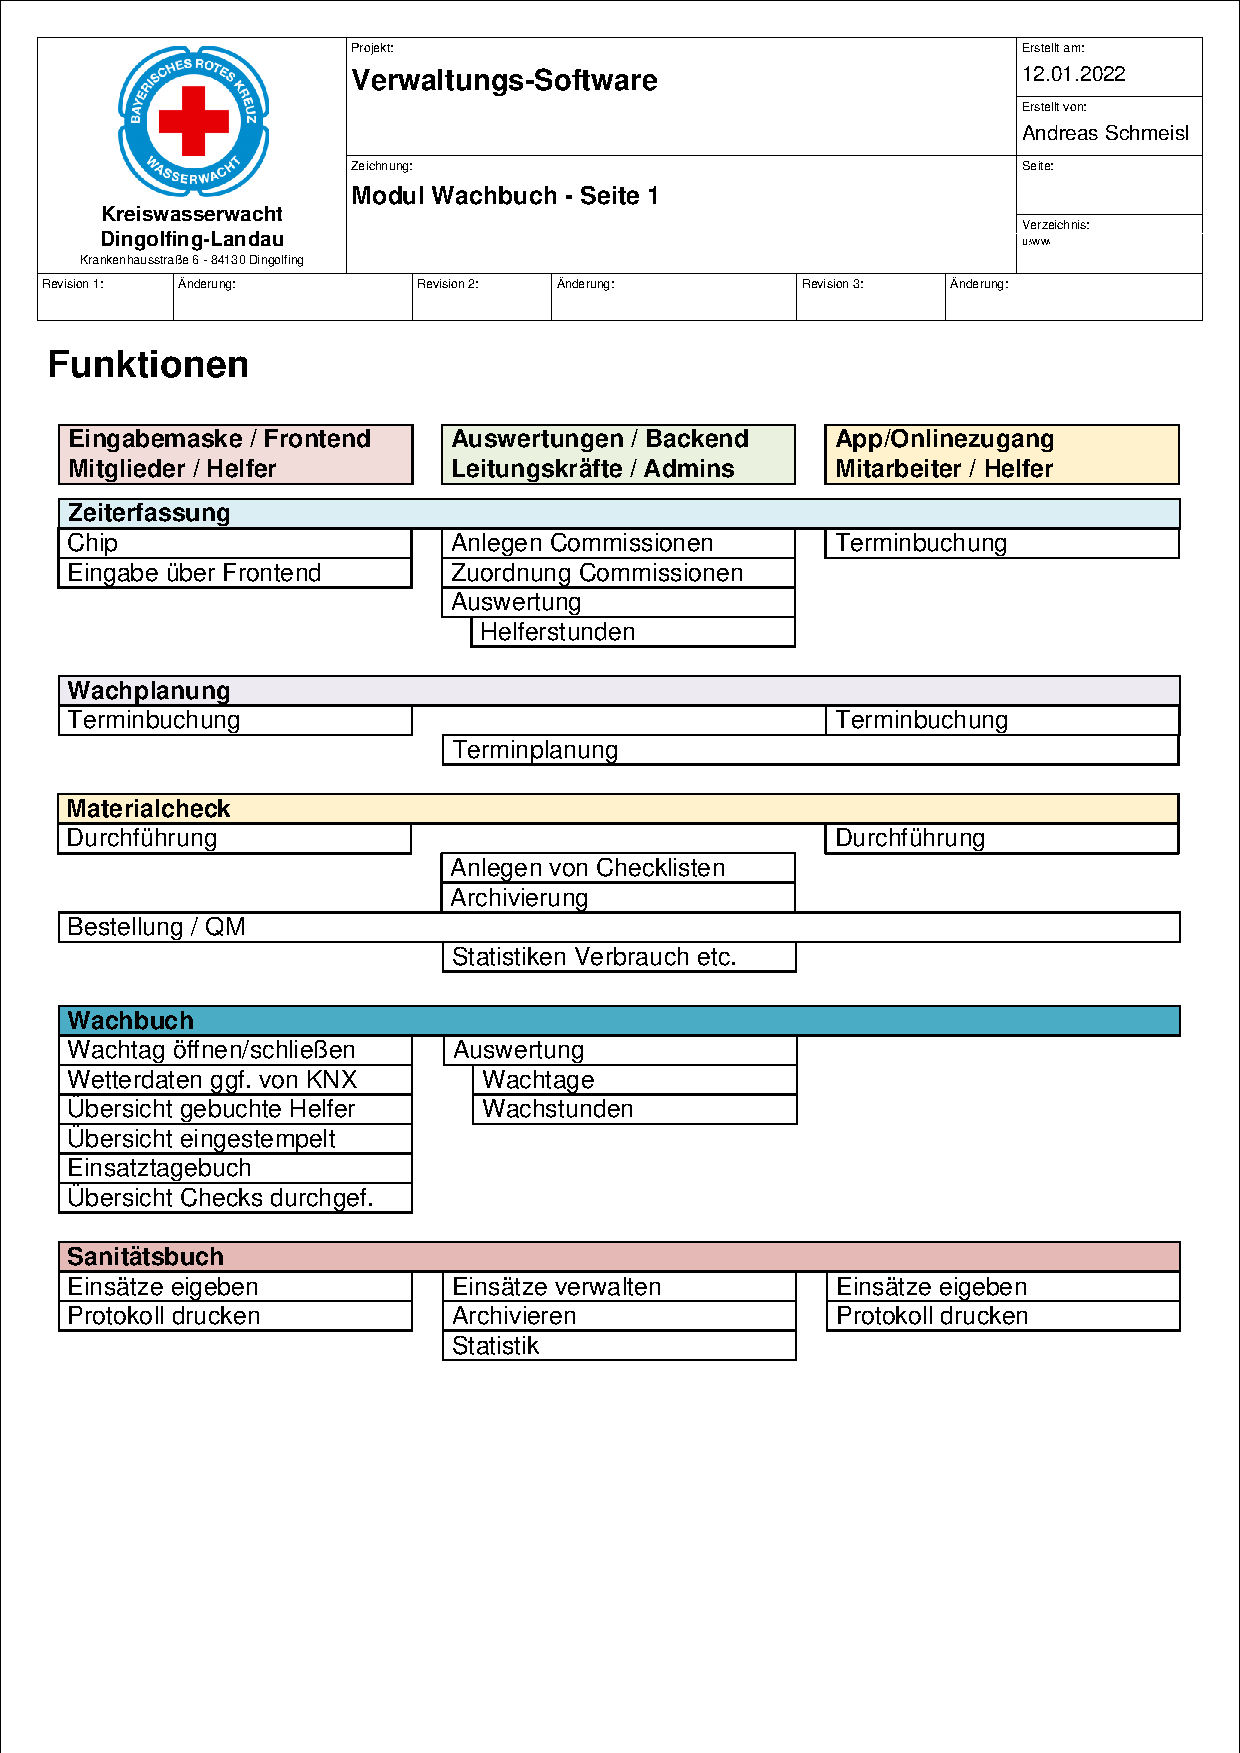
\includepdf[pages=1,scale=0.65, offset=0 0,pagecommand={\chapter{Anhang}\section{Initialer Entwurf}\thispagestyle{plain}}
]{Anlagen/WSM_Software_Modul_Wachbuch.pdf}

\includepdf[pages=2, scale=0.75,pagecommand={\thispagestyle{plain}}]{Anlagen/WSM_Software_Modul_Wachbuch.pdf}

\begin{figure}[H]
\centering
    \includegraphics[page=3,scale=0.75]{Anlagen/WSM_Software_Modul_Wachbuch.pdf}
  \caption{Initialer Entwurf}
  \label{fig:initial}
\end{figure}

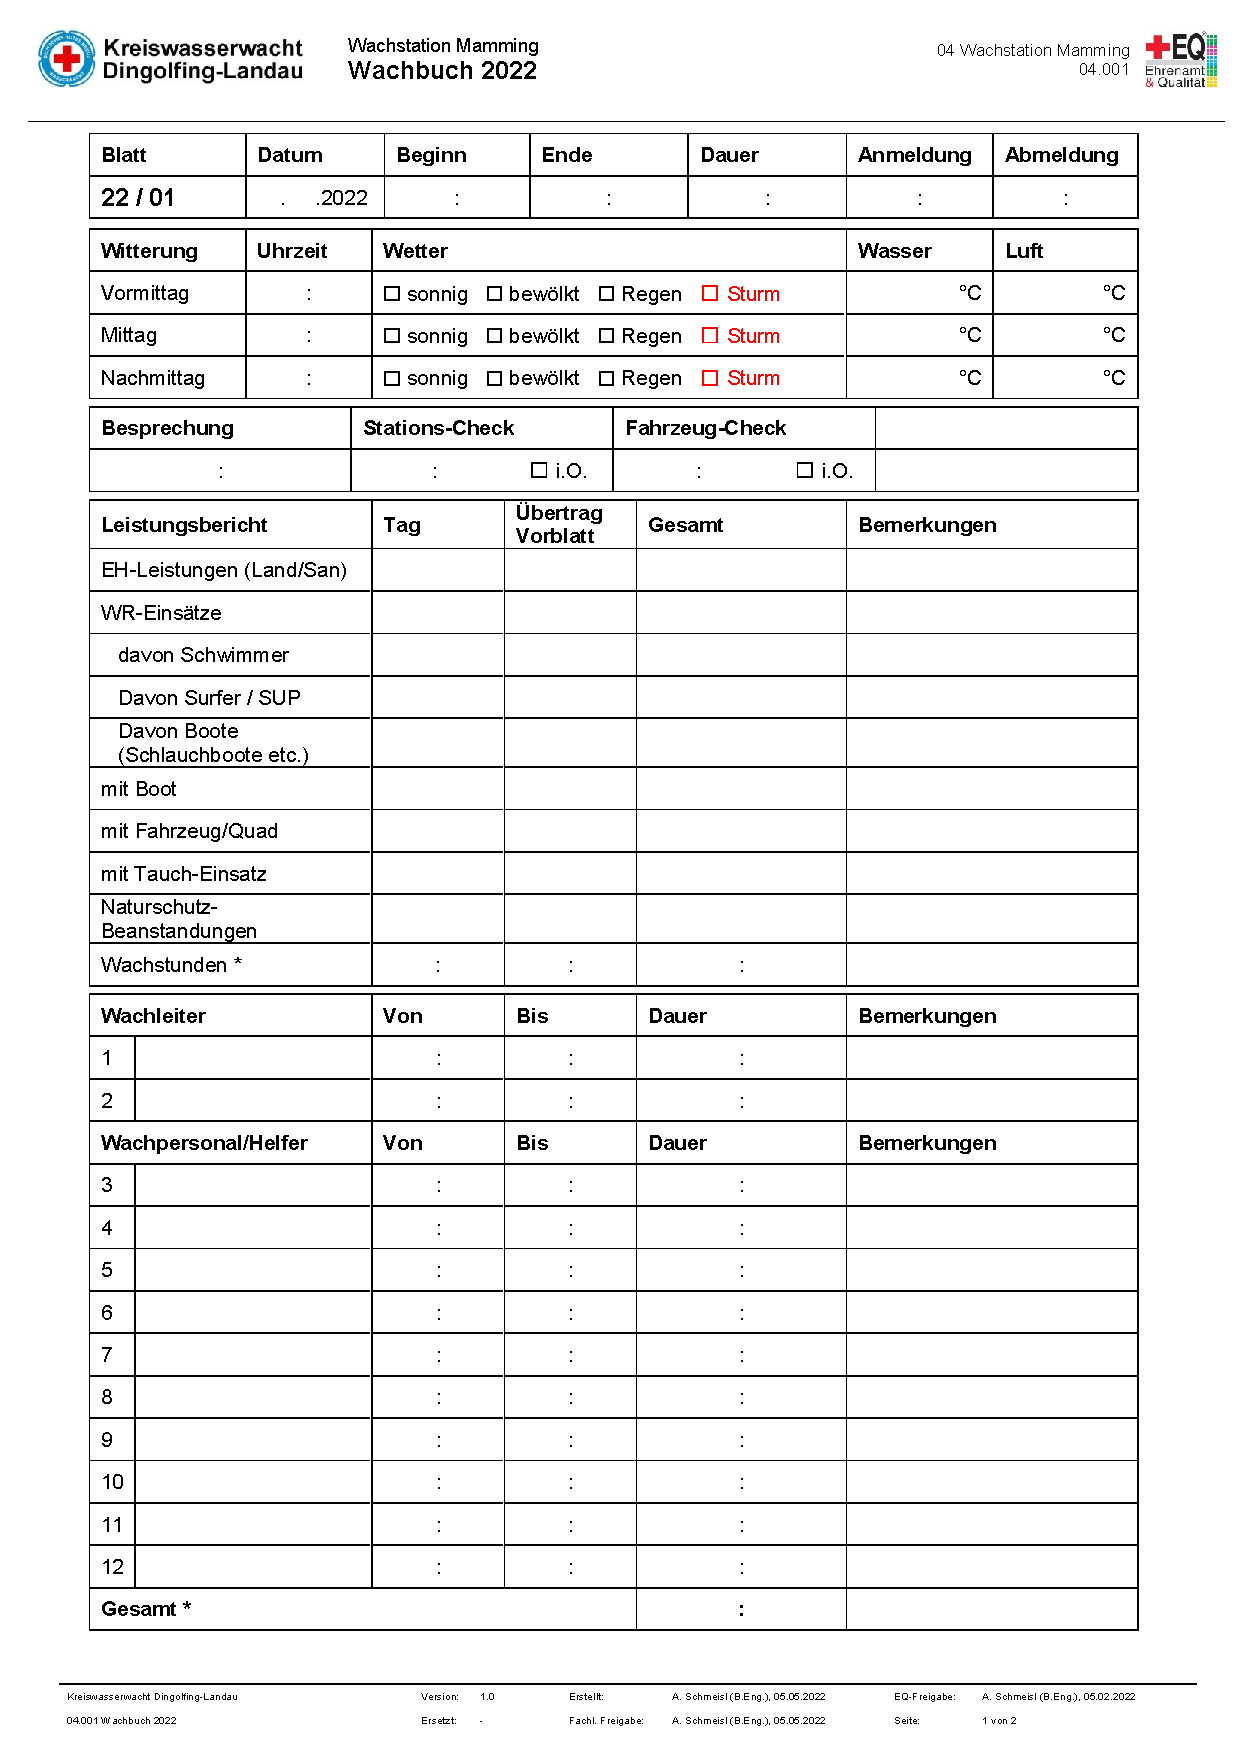
\includepdf[pages=1,scale=0.65, offset=0 0,pagecommand={\section{Wachbuch Papier}\thispagestyle{plain}}
]{Anlagen/wachbuchPapier.pdf}

\begin{figure}[H]
\centering
    \includegraphics[page=2,scale=0.75]{Anlagen/wachbuchPapier.pdf}
  \caption{Wachbuch Papier}
  \label{fig:wachbuchpapier}
\end{figure}

\begin{figure}[H]
\centering
    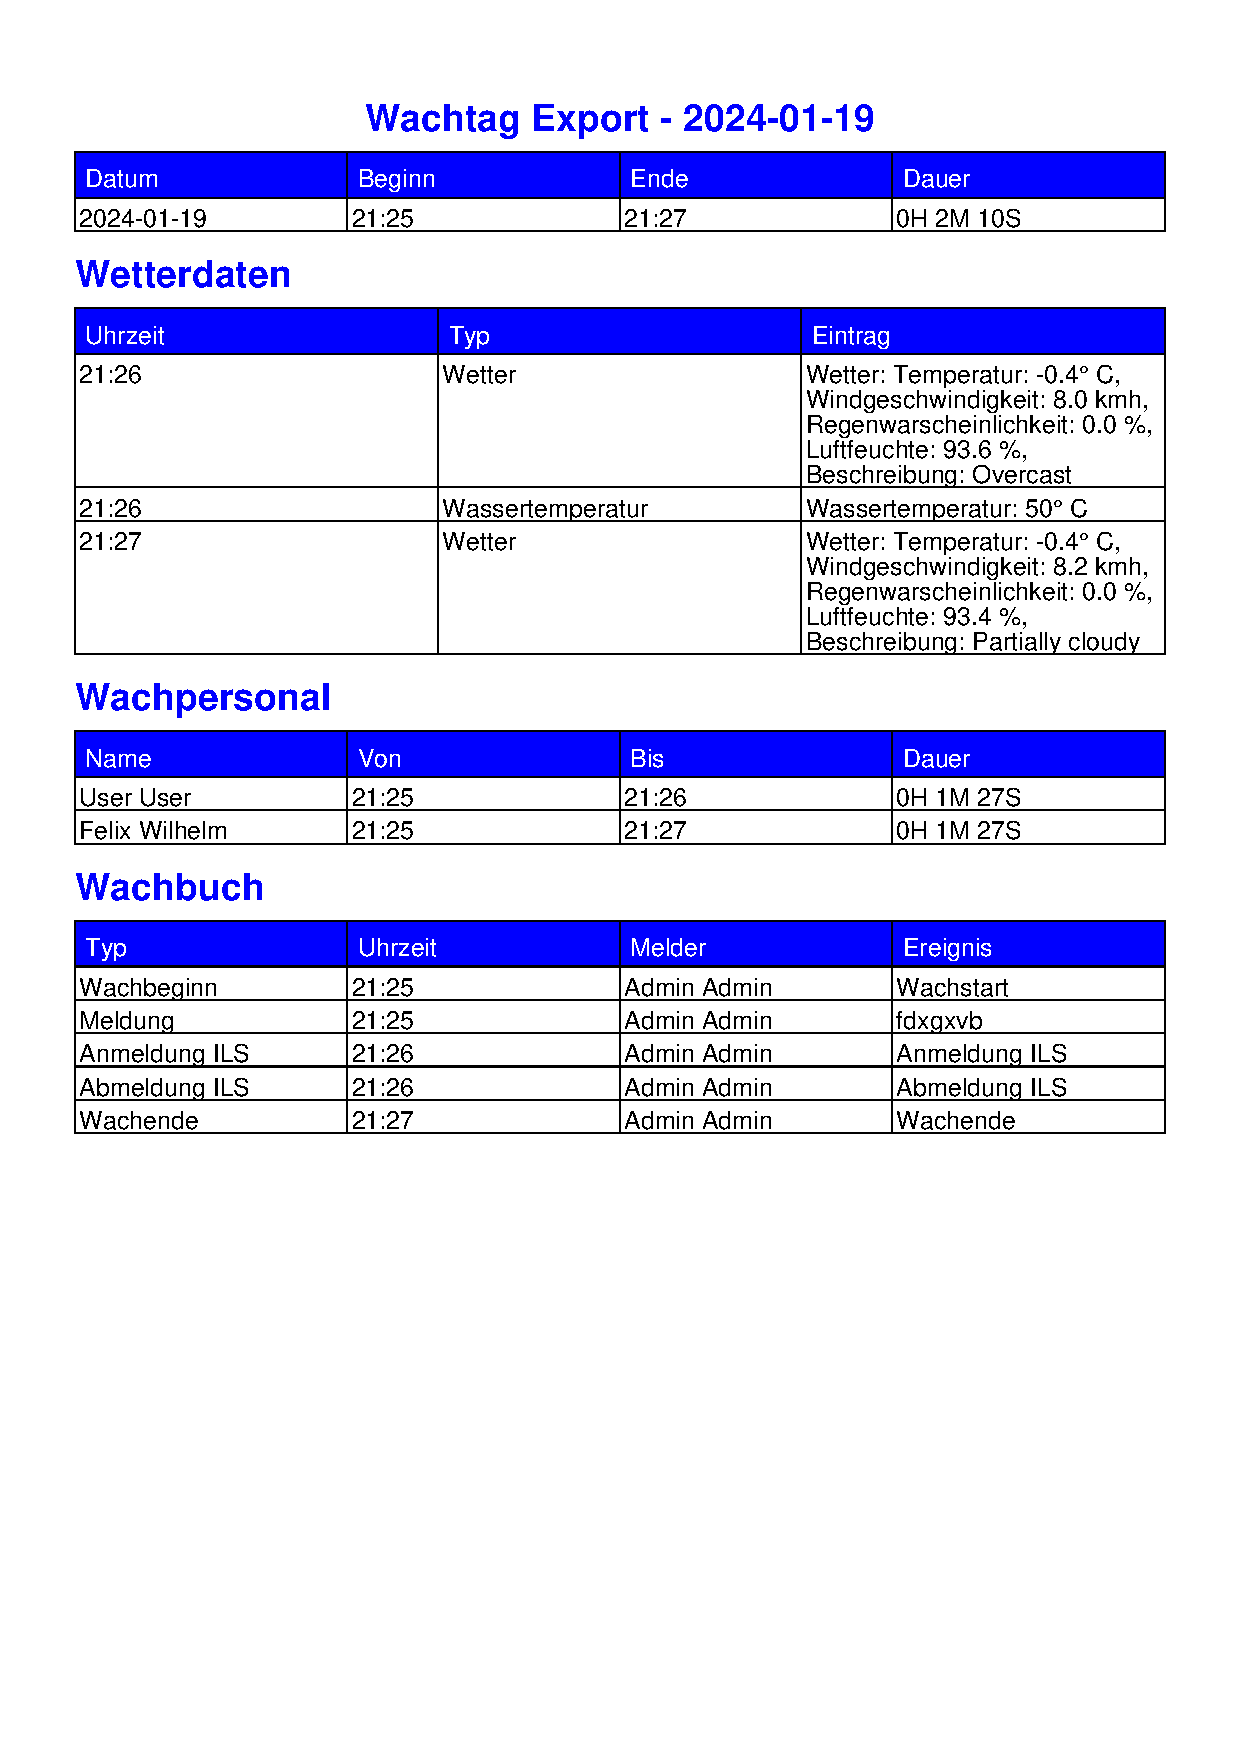
\includegraphics[page=1,scale=0.75]{Anlagen/Anwendung/10WachtagExport.pdf}
  \caption{Wachtag Export}
  \label{fig:wachtagexport}
\end{figure}

\end{appendix}

	 
% References (Literaturverzeichnis):
\bibliographystyle{alpha}
\bibliography{Literatur}


\includepdf[
    pages=1,
    frame,
    scale=.75]
    {Anlagen/EidesstattlicheErklaerung.pdf}

%%%%%%%%%%%%%%%%%%%%%%%%%%%%%%%%%%%%%%%%%%%%%%%%%%%%%%%%%%%%
\end{document}
